\documentclass[twoside]{article}

% CONTROLS
\newif\ifappendix
	\appendixtrue
	% \appendixfalse
\newif\ifbody\bodytrue
\newif\ifmarginprooflinks
	% \marginprooflinkstrue
	\marginprooflinksfalse

\relax %Header
		
	\usepackage[accepted]{aistats2022} % aistats formatting
	    % If your paper is accepted, change the options for the package
	    % aistats2022 as follows:
	    %
	    %\usepackage[accepted]{aistats2022}
	    %
	    % This option will print headings for the title of your paper and
	    % headings for the authors names, plus a copyright note at the end of
	    % the first column of the first page.

	    % If you set papersize explicitly, activate the following three lines:
	    %\special{papersize = 8.5in, 11in}
	    %\setlength{\pdfpageheight}{11in}
	    %\setlength{\pdfpagewidth}{8.5in}

		\usepackage[american]{babel}
		\usepackage{csquotes}
		\usepackage[backend=biber, style=authoryear]{biblatex}
		\DeclareLanguageMapping{american}{american-apa}
		% \usepackage[backend=biber,style=authoryear,hyperref=true]{biblatex}
		\addbibresource{refs.bib}
		% \listfiles

		\DeclareFieldFormat{citehyperref}{%
		  \DeclareFieldAlias{bibhyperref}{noformat}% Avoid nested links
		  \bibhyperref{#1}}

		\DeclareFieldFormat{textcitehyperref}{%
		  \DeclareFieldAlias{bibhyperref}{noformat}% Avoid nested links
		  \bibhyperref{%
		    #1%
		    \ifbool{cbx:parens}
		      {\bibcloseparen\global\boolfalse{cbx:parens}}
		      {}}}

		\savebibmacro{cite}
		\savebibmacro{textcite}

		\renewbibmacro*{cite}{%
		  \printtext[citehyperref]{%
		    \restorebibmacro{cite}%
		    \usebibmacro{cite}}}

		\renewbibmacro*{textcite}{%
		  \ifboolexpr{
		    ( not test {\iffieldundef{prenote}} and
		      test {\ifnumequal{\value{citecount}}{1}} )
		    or
		    ( not test {\iffieldundef{postnote}} and
		      test {\ifnumequal{\value{citecount}}{\value{citetotal}}} )
		  }
		    {\DeclareFieldAlias{textcitehyperref}{noformat}}
		    {}%
		  \printtext[textcitehyperref]{%
		    \restorebibmacro{textcite}%
		    \usebibmacro{textcite}}}

		% \renewbibmacro*{cite}{%
		% 	\printtext[bibhyperref]{%
		%     \iffieldundef{shorthand}
		%       {\ifthenelse{\ifnameundef{labelname}\OR\iffieldundef{labelyear}}
		%          {\usebibmacro{cite:label}%
		%           \setunit{\printdelim{nonameyeardelim}}}
		%          {\printnames{labelname}%
		%           \setunit{\printdelim{nameyeardelim}}}%
		%        \usebibmacro{cite:labeldate+extradate}}
		%       {\usebibmacro{cite:shorthand}}}}
		%
		% \renewbibmacro*{citeyear}{%
		%   \printtext[bibhyperref]{%
		%     \iffieldundef{shorthand}
		%       {\iffieldundef{labelyear}
		%          {\usebibmacro{cite:label}}
		%          {\usebibmacro{cite:labeldate+extradate}}}
		%       {\usebibmacro{cite:shorthand}}}}
		%
		% \renewbibmacro*{textcite}{%
		%   \ifnameundef{labelname}
		%     {\iffieldundef{shorthand}
		%        {\printtext[bibhyperref]{%
		%           \usebibmacro{cite:label}}%
		%         \setunit{%
		%           \global\booltrue{cbx:parens}%
		%           \printdelim{nonameyeardelim}\bibopenparen}%
		%         \ifnumequal{\value{citecount}}{1}
		%           {\usebibmacro{prenote}}
		%           {}%
		%         \printtext[bibhyperref]{\usebibmacro{cite:labeldate+extradate}}}
		%        {\printtext[bibhyperref]{\usebibmacro{cite:shorthand}}}}
		%     {\printtext[bibhyperref]{\printnames{labelname}}%
		%      \setunit{%
		%        \global\booltrue{cbx:parens}%
		%        \printdelim{nameyeardelim}\bibopenparen}%
		%      \ifnumequal{\value{citecount}}{1}
		%        {\usebibmacro{prenote}}
		%        {}%
		%      \usebibmacro{citeyear}}}
		%
		% \renewbibmacro*{cite:shorthand}{%
		%   \printfield{shorthand}}
		%
		% \renewbibmacro*{cite:label}{%
		%   \iffieldundef{label}
		%     {\printfield[citetitle]{labeltitle}}
		%     {\printfield{label}}}
		%
		% \renewbibmacro*{cite:labeldate+extradate}{%
		%   \printlabeldateextra}
		% \DeclareCiteCommand{\parencite}
		%   {\usebibmacro{prenote}}
		%   {\usebibmacro{citeindex}%
		%    \printtext[bibhyperref]{(\usebibmacro{cite})}}
		%   {\multicitedelim}
		%   {\usebibmacro{postnote}}
		\DeclareCiteCommand{\brakcite}
		  {\usebibmacro{prenote}}
		  {\usebibmacro{citeindex}%
		   \printtext[bibhyperref]{[\usebibmacro{cite}]}}
		  {\multicitedelim}
		  {\usebibmacro{postnote}}

		% If you use natbib package, activate the following three lines:
	    % \usepackage[round]{natbib}
	    % \renewcommand{\bibname}{References}
	    % \renewcommand{\bibsection}{\subsubsection*{\bibname}}

	    % If you use BibTeX in apalike style, activate the following line:
	    % \bibliographystyle{apalike}

	\usepackage[dvipsnames]{xcolor}
	\usepackage{tikz}
		\usetikzlibrary{positioning,fit,calc, decorations, arrows, shapes, shapes.geometric}
		\usetikzlibrary{cd}

		%%%%%%%%%%%%
		\tikzset{AmpRep/.style={ampersand replacement=\&}}
		\tikzset{center base/.style={baseline={([yshift=-.8ex]current bounding box.center)}}}
		\tikzset{paperfig/.style={center base,scale=0.9, every node/.style={transform shape}}}

		% Node Stylings
		\tikzset{dpadded/.style={rounded corners=2, inner sep=0.7em, draw, outer sep=0.3em, fill={black!50}, fill opacity=0.08, text opacity=1}}
		\tikzset{dpad0/.style={outer sep=0.05em, inner sep=0.3em, draw=gray!75, rounded corners=4, fill=black!08, fill opacity=1, align=center}}
		\tikzset{dpadinline/.style={outer sep=0.05em, inner sep=2.5pt, rounded corners=2.5pt, draw=gray!75, fill=black!08, fill opacity=1, align=center, font=\small}}

	 	\tikzset{dpad/.style args={#1}{every matrix/.append style={nodes={dpadded, #1}}}}
		\tikzset{light pad/.style={outer sep=0.2em, inner sep=0.5em, draw=gray!50}}

		\tikzset{arr/.style={draw, ->, thick, shorten <=3pt, shorten >=3pt}}
		\tikzset{arr0/.style={draw, ->, thick, shorten <=0pt, shorten >=0pt}}
		\tikzset{arr1/.style={draw, ->, thick, shorten <=1pt, shorten >=1pt}}
		\tikzset{arr2/.style={draw, ->, thick, shorten <=2pt, shorten >=2pt}}

		\newcommand\cmergearr[5][]{
			\draw[arr, #1, -] (#2) -- (#5) -- (#3);
			\draw[arr, #1, shorten <=0] (#5) -- (#4);
			}
		\newcommand\mergearr[4][]{
			\coordinate (center-#2#3#4) at (barycentric cs:#2=1,#3=1,#4=1.2);
			\cmergearr[#1]{#2}{#3}{#4}{center-#2#3#4}
			}
		\newcommand\cunmergearr[5][]{
			\draw[arr, #1, -, shorten >=0] (#2) -- (#5);
			\draw[arr, #1, shorten <=0] (#5) -- (#3);
			\draw[arr, #1, shorten <=0] (#5) -- (#4);
			}
		\newcommand\unmergearr[4][]{
			\coordinate (center-#2#3#4) at (barycentric cs:#2=1.2,#3=1,#4=1);
			\cunmergearr[#1]{#2}{#3}{#4}{center-#2#3#4}
			}
		\newcommand\lab[1]{(#1)(lab-#1)}
		\tikzset{alternative/.style args={#1|#2|#3}{name=#1, circle, fill, inner sep=1pt,label={[name={lab-#1},gray!30!black, inner sep=1pt]#3:\scriptsize #2}} }
		\tikzset{tpt/.style args={#1|#2}{alternative={#1|#2|below}} }
		\tikzset{Dom/.style args={#1[#2] (#3) around #4}{dpadded, name=#3, label={[name={lab-#3},align=center,label distance=-1.9em, shading = axis, top color=white, bottom color=black!04, #2]120:#1}, fit={ #4 }, inner sep=0.5em}}

	\relax % Most packages
	    % \usepackage[utf8]{inputenc}
	    \usepackage{mathtools}
	    \usepackage{amssymb}
			\DeclareMathSymbol{\shortminus}{\mathbin}{AMSa}{"39}
	    % \usepackage{parskip}
	    % \usepackage{algorithm}
	    \usepackage{bbm}
		\usepackage{lmodern}
		% \usepackage{times}
	    \usepackage{faktor}
	    % \usepackage{booktabs}
		% \usepackage[margin=1in]{geometry}
	    \usepackage{graphicx}
	    \usepackage{scalerel}
	    \usepackage{enumitem}
	    \usepackage{nicefrac}\let\nf\nicefrac

	    \usepackage{color}
	    %\usepackage{stmaryrd}
	    \usepackage{hyperref} % Load before theorems...
	        \hypersetup{colorlinks=true, linkcolor=blue!75!black, urlcolor=magenta, citecolor=green!50!black}

	\usepackage{amsthm,thmtools} % Theorem Packages
		\usepackage[noabbrev,nameinlink,capitalize]{cleveref}
	    \theoremstyle{plain}
	    \newtheorem{theorem}{Theorem}
		\newtheorem{coro}{Corollary}[theorem]
	    \newtheorem{prop}[theorem]{Proposition}
	    \newtheorem{claim}{Claim}
	    \newtheorem{remark}{Remark}
	    \newtheorem{lemma}[theorem]{Lemma}
	    \theoremstyle{definition}
	    % \newtheorem{defn}{Definition}
	    % \declaretheorem[name=Definition]{defn}
	    \declaretheorem[name=Definition, qed=$\square$]{defn}

		\crefname{defn}{Definition}{Definitions}
		\crefname{prop}{Proposition}{Propositions}

	\relax %%%%%%%%% GENERAL MACROS %%%%%%%%
	    \let\Horig\H
		\let\H\relax
		\DeclareMathOperator{\H}{\mathrm{H}} % Entropy
		\DeclareMathOperator{\I}{\mathrm{I}} % Information
		\DeclareMathOperator*{\Ex}{\mathbb{E}} % Expectation
		\DeclareMathOperator*{\EX}{\scalebox{1.5}{$\mathbb{E}$}}

	    \newcommand{\mat}[1]{\mathbf{#1}}
	    \DeclarePairedDelimiterX{\infdivx}[2]{(}{)}{%
			#1\;\delimsize\|\;#2%
		}
		\newcommand{\thickD}{I\mkern-8muD}
		\newcommand{\kldiv}{\thickD\infdivx}
		\newcommand{\tto}{\rightarrow\mathrel{\mspace{-15mu}}\rightarrow}

		\newcommand{\datadist}[1]{\Pr\nolimits_{#1}}
		% \newcommand{\datadist}[1]{p_\text{data}}

		\makeatletter
		\newcommand{\subalign}[1]{%
		  \vcenter{%
		    \Let@ \restore@math@cr \default@tag
		    \baselineskip\fontdimen10 \scriptfont\tw@
		    \advance\baselineskip\fontdimen12 \scriptfont\tw@
		    \lineskip\thr@@\fontdimen8 \scriptfont\thr@@
		    \lineskiplimit\lineskip
		    \ialign{\hfil$\m@th\scriptstyle##$&$\m@th\scriptstyle{}##$\hfil\crcr
		      #1\crcr
		    }%
		  }%
		}
		\makeatother
		\newcommand\numberthis{\addtocounter{equation}{1}\tag{\theequation}}

	\relax %%%%%%%%%   PDG  MACROS   %%%%%%%%
		\newcommand{\ssub}[1]{_{\!_{#1}\!}}
		% \newcommand{\bp}[1][L]{\mat{p}_{\!_{#1}\!}}
		% \newcommand{\bP}[1][L]{\mat{P}_{\!_{#1}\!}}
		\newcommand{\bp}[1][L]{\mat{p}\ssub{#1}}
		\newcommand{\bP}[1][L]{\mat{P}\ssub{#1}}
		\newcommand{\V}{\mathcal V}
		\newcommand{\N}{\mathcal N}
		\newcommand{\Ed}{\mathcal E}

	    \newcommand{\balpha}{\boldsymbol\alpha}
	    \newcommand{\bbeta}{\boldsymbol\beta}

		\DeclareMathAlphabet{\mathdcal}{U}{dutchcal}{m}{n}
		\DeclareMathAlphabet{\mathbdcal}{U}{dutchcal}{b}{n}
		\newcommand{\dg}[1]{\mathbdcal{#1}}
		\newcommand{\PDGof}[1]{{\dg M}_{#1}}
		\newcommand{\UPDGof}[1]{{\dg N}_{#1}}
		\newcommand\VFE{\mathit{V\mkern-4mu F\mkern-4.5mu E}}

		\newcommand\Inc{\mathit{Inc}}
		\newcommand{\IDef}[1]{\mathit{IDef}_{\!#1}}
		% \newcommand{\ed}[3]{%
		% 	\mathchoice%
		% 	{#2\overset{\smash{\mskip-5mu\raisebox{-3pt}{${#1}$}}}{\xrightarrow{\hphantom{\scriptstyle {#1}}}} #3} %display style
		% 	{#2\overset{\smash{\mskip-5mu\raisebox{-3pt}{$\scriptstyle {#1}$}}}{\xrightarrow{\hphantom{\scriptstyle {#1}}}} #3}% text style
		% 	{#2\overset{\smash{\mskip-5mu\raisebox{-3pt}{$\scriptscriptstyle {#1}$}}}{\xrightarrow{\hphantom{\scriptscriptstyle {#1}}}} #3} %script style
		% 	{#2\overset{\smash{\mskip-5mu\raisebox{-3pt}{$\scriptscriptstyle {#1}$}}}{\xrightarrow{\hphantom{\scriptscriptstyle {#1}}}} #3}} %scriptscriptstyle
		\newcommand{\ed}[3]{#2%
		  \overset{\smash{\mskip-5mu\raisebox{-1pt}{$\scriptscriptstyle
		        #1$}}}{\rightarrow} #3}

	    \newcommand{\nhphantom}[2]{\sbox0{\kern-2%
			\nulldelimiterspace$\left.\delimsize#1\vphantom{#2}\right.$}\hspace{-.97\wd0}}
			% \nulldelimiterspace$\left.\delimsize#1%
			% \vrule depth\dp#2 height \ht#2 width0pt\right.$}\hspace{-.97\wd0}}
		\makeatletter
		\newsavebox{\abcmycontentbox}
		\newcommand\DeclareDoubleDelim[5]{
		    \DeclarePairedDelimiterXPP{#1}[1]%
				{% box must be saved in this pre code
					\sbox{\abcmycontentbox}{\ensuremath{##1}}%
				}{#2}{#5}{}%
			    %%% Correct spacing, but doesn't work with externalize.
				% {\nhphantom{#3}{##1}\hspace{1.2pt}\delimsize#3\mathopen{}##1\mathclose{}\delimsize#4\hspace{1.2pt}\nhphantom{#4}{##1}}
				%%% Fast, but wrong spacing.
				% {\nhphantom{#3}{~}\hspace{1.2pt}\delimsize#3\mathopen{}##1\mathclose{}\delimsize#4\hspace{1.2pt}\nhphantom{#4}{~}}
				%%% with savebox.
			    {%
					\nhphantom{#3}{\usebox\abcmycontentbox}%
					\hspace{1.2pt} \delimsize#3%
					\mathopen{}\usebox{\abcmycontentbox}\mathclose{}%
					\delimsize#4\hspace{1.2pt}%
					\nhphantom{#4}{\usebox\abcmycontentbox}%
				}%
		}
		\makeatother
		\DeclareDoubleDelim
			\SD\{\{\}\}
		\DeclareDoubleDelim
			\bbr[[]]
		% \DeclareDoubleDelim
		% 	\aar\langle\langle\rangle\rangle
		\makeatletter
		\newsavebox{\aar@content}
		\newcommand\aar{\@ifstar\aar@one@star\aar@plain}
		\newcommand\aar@one@star{\@ifstar\aar@resize{\aar@plain*}}
		\newcommand\aar@resize[1]{\sbox{\aar@content}{#1}\scaleleftright[3.8ex]
			{\Biggl\langle\!\!\!\!\Biggl\langle}{\usebox{\aar@content}}
			{\Biggr\rangle\!\!\!\!\Biggr\rangle}}
		\DeclareDoubleDelim
			\aar@plain\langle\langle\rangle\rangle
		\makeatother


		% \DeclarePairedDelimiterX{\aar}[1]{\langle}{\rangle}
		% 	{\nhphantom{\langle}{#1}\hspace{1.2pt}\delimsize\langle\mathopen{}#1\mathclose{}\delimsize\rangle\hspace{1.2pt}\nhphantom{\rangle}{#1}}

	\relax %%%%% restatables and links
		% \usepackage{xstring} % for expandarg
		\usepackage{xpatch}
		\makeatletter
		\xpatchcmd{\thmt@restatable}% Edit \thmt@restatable
		   {\csname #2\@xa\endcsname\ifx\@nx#1\@nx\else[{#1}]\fi}% Replace this code
		   % {\ifthmt@thisistheone\csname #2\@xa\endcsname\typeout{oiii[#1;#2\@xa;#3;\csname thmt@stored@#3\endcsname]}\ifx\@nx#1\@nx\else[#1]\fi\else\csname #2\@xa\endcsname\fi}% with this code
		   {\ifthmt@thisistheone\csname #2\@xa\endcsname\ifx\@nx#1\@nx\else[{#1}]\fi
		   \else\fi}
		   {}{\typeout{FIRST PATCH TO THM RESTATE FAILED}} % execute on success/failure
		\xpatchcmd{\thmt@restatable}% A second edit to \thmt@restatable
		   {\csname end#2\endcsname}
		   {\ifthmt@thisistheone\csname end#2\endcsname\else\fi}
		   {}{\typeout{FAILED SECOND THMT RESTATE PATCH}}

		% \def\onlyaftercolon#1:#2{#2}
		\newcommand{\recall}[1]{\medskip\par\noindent{\bf \Cref{thmt@@#1}.} \begingroup\em \noindent
		   \expandafter\csname#1\endcsname* \endgroup\par\smallskip}

	   	\setlength\marginparwidth{1.55cm}
		\newenvironment{linked}[3][]{%
			\def\linkedproof{#3}%
			\def\linkedtype{#2}%
			% \reversemarginpar
			% \marginpar{%
			% \vspace{1.1em}
			% % \hspace{2em}
			% 	% \raggedleft
			% 	\raggedright
			% 	\hyperref[proof:\linkedproof]{%
			% 	\color{blue!50!white}
			% 	\scaleleftright{$\Big[$}{\,{\small\raggedleft\tt\begin{tabular}{@{}c@{}} proof of \\\linkedtype~\ref*{\linkedtype:\linkedproof}\end{tabular}}\,}{$\Big]$}}
			% 	}%
	        % \restatable[#1]{#2}{#2:#3}\label{#2:#3}%
			\ifmarginprooflinks
			\marginpar{%
				% \vspace{-3em}% %% for bottom
				\vspace{1.5em}
				\centering%
				\hyperref[proof:\linkedproof]{%
	            % \hyperref[proof:#3]{
				\color{blue!30!white}%
				\scaleleftright{$\Big[$}{\,\mbox{\footnotesize\centering\tt\begin{tabular}{@{}c@{}}
					% proof of \\\,\linkedtype~\ref*{\linkedtype:\linkedproof}
					link to\\[-0.15em]
					proof
				\end{tabular}}\,}{$\Big]$}}~
				}%
			\fi
	        \restatable[#1]{#2}{#2:#3}\label{#2:#3}%
	        }%
			{\endrestatable%
			}
		\makeatother
			\newcounter{proofcntr}
			\newenvironment{lproof}{\begin{proof}\refstepcounter{proofcntr}}{\end{proof}}

			\usepackage{cancel}
			\newcommand{\Cancel}[2][black]{{\color{#1}\cancel{\color{black}#2}}}

			\usepackage{tcolorbox}
			\tcbuselibrary{most}
			\tcolorboxenvironment{lproof}{
				% fonttitle=\bfseries,
				% top=0.5em,
				enhanced,
				parbox=false,
				boxrule=0pt,
				frame hidden,
				borderline west={4pt}{0pt}{blue!20!black!40!white},
				% coltext={blue!20!black!60!white},
				colback={blue!20!black!05!white},
				sharp corners,
				breakable,
				% bottomsep at break=4cm,
				% enlarge bottom at break by=-4cm,
				% topsep at break=3cm,
				% enlarge top at break by=-3cm
			}
			% \usepackage[framemethod=TikZ]{mdframed}
			% \surroundwithmdframed[ % lproof
			% 	   topline=false,
			% 	   linewidth=3pt,
			% 	   linecolor=gray!20!white,
			% 	   rightline=false,
			% 	   bottomline=false,
			% 	   leftmargin=0pt,
			% 	   % innerleftmargin=5pt,
			% 	   skipabove=\medskipamount,
			% 	   skipbelow=\medskipamount
			% 	]{lproof}
		%oli16: The extra space was because there was extra space in the paragraph, not
		%because this length was too big. By breaking arrays, everything will be better.
		\newcommand{\begthm}[3][]{\begin{#2}[{name=#1},restate=#3,label=#3]}

	\relax %TODOs and footnotes
	    \newcommand{\TODO}[1][INCOMPLETE]{{\centering\Large\color{red}$\langle$~\texttt{#1}~$\rangle$\par}}
	    \newcommand{\dfootnote}[1]{%
	        \let\oldthefootnote=\thefootnote%
	        % \addtocounter{footnote}{-1}%
			\setcounter{footnote}{999}
	        \renewcommand{\thefootnote}{\textdagger}%
	        \footnote{#1}%
	        \let\thefootnote=\oldthefootnote%
	    }
		\newcommand{\dfootnotemark}{
			\footnotemark[999]
		}

\begin{document}

% If your paper is accepted and the title of your paper is very long,
% the style will print as headings an error message. Use the following
% command to supply a shorter title of your paper so that it can be
% used as headings.
%
%\runningtitle{I use this title instead because the last one was very long}

% If your paper is accepted and the number of authors is large, the
% style will print as headings an error message. Use the following
% command to supply a shorter version of the authors names so that
% they can be used as headings (for example, use only the surnames)
%
%\runningauthor{Surname 1, Surname 2, Surname 3, ...., Surname n}

\runningtitle{Loss as the Inconsistency of a PDG: Choose Your Model, Not Your Loss}
% \runningtitle{Loss as Inconsistency: Choose your Model, not your Loss}
% \runningtitle{Choose your Model, not your Loss}
\twocolumn[
	%%  Title objectives (might not be simultaneously satisfiable)
	%%    -focus on inconsistency.  -Naturality. -Not over-reaching.
	%%
	% \aistatstitle{(PDG) Inconsistency: the Universal Loss}
	% \aistatstitle{Choose your Model, not your Loss:}
	% \aistatstitle{Loss Functions are the Shadows of Inconsistent Models}
	% \aistatstitle{Loss Functions are the Shadows of Inconsistent Models (Choose your Model, not your Loss)}
	% \aistatstitle{Loss Functions are the Shadows of Inconsistent Models}
	% \aistatstitle{Inconsistency, the Universal Loss Fuction: How Loss is but the Shadow of an Inconsistent Model}
	% \aistatstitle{Inconsistency, the Universal Loss Fuction: Our Favorite Objectives are but  Shadows of Inconsistent Models}
	% \aistatstitle{The One True Loss: How Our Objectives are but Shadows of Inconsistent Models}
	%
	% \aistatstitle{Probabilistic Dependency Graphs: Model Inconsistency as the Universal Loss Function}
	% \aistatstitle{Inconsistency, the Universal Loss Fuction: Our Favorite Objectives are mere shadows of Probabilistic Dependency Graphs}
	% \aistatstitle{Choose your Model, not your Loss Function: Objectives are the Shadows cast by Inconsistent Probabilistic Dependency Graphs}
	% \aistatstitle{Loss Functions are mere Shadows of Probabilistic Dependency Graphs: Choose your Model, not your Loss}
	% \aistatstitle{Inconsistency from Probabilistic Dependency Graphs: Choose your Model not Your Loss.}
	% \aistatstitle{Loss Functions from Probabilistic Dependency Graphs: Choose your Model not Your Loss.}
	% \aistatstitle{ The Shadows of an Inconsistent Probabilistic Dependency Graphs: \\
		% Choose your Model, not your Loss Function}
	\aistatstitle{ Loss as the Inconsistency of a Probabilistic Dependency Graph: \\ Choose Your Model, Not Your Loss Function}
	% \aistatstitle{ Probabilistic Dependency Graph Inconsistency, the Natural Loss: \\ Choose your Model, not your Loss Function}
	\aistatsauthor{ Oliver E. Richardson }
	\aistatsaddress{ Cornell University }
]

\begin{abstract}
    % The Abstract paragraph should be indented 0.25 inch (1.5 picas) on
    % both left and right-hand margins. Use 10~point type, with a vertical
    % spacing of 11~points. The \textbf{Abstract} heading must be centered,
    % bold, and in point size 12. Two line spaces precede the
    % Abstract. The Abstract must be limited to one paragraph.
    % I will argue that minimizing PDG inconsistency is actually much more broadly useful, and in particular show that many standard loss functions arise as the inconsistency of the natural PDG describing the appropriate scenario.  We will then see how the extra structure of the underlying PDGs gives a rich visual proof language for reasoning about the relationships between objectives.
    In a world blessed with a great diversity of loss functions,
    % In a world with a great diversity of loss functions,
    % we argue that that choice between them is not a matter of taste, but a modeling assumption.
    we argue that that choice between them is not a matter of taste or pragmatics, but of model.
	%joe1: This is the first of many places where you assume the reader
	%knows what you know, although that's unlikely to be true.    The
	%reader won't know that we can talk about the inconsistency of a PDG.
	    %Added next sentence
		% We can associate with each PDG its \emph{inconsistency}, a measure of
		% the degree to which the PDG is inconsistent.
	%oli1: merged with previous sentence
	% Probabilistic Depencency Graphs (PDGs) are probabilistic models which can be inconsistent, and come equipped with a measure of inconsistency.
	Probabilistic depencency graphs (PDGs) are probabilistic models that come equipped with a measure of ``inconsistency''.
    We prove that many standard loss functions arise as the inconsistency of
	%joe1: I doubt it's unique in general
	%    the natural PDG describing the scenario at hand, and corroborate
    %oli1: There's not a unique PDG that gives rise to the functional, but up to some kind of isomorphism, I think there is a unique one that represents the scenario properly. I want to emphasize the fact that less choice is required...
	% the natural PDG describing the appropriate scenario.
	%
    a natural PDG describing the appropriate scenario%
	%.
	, and use the same approach
	% The same approach can be used
	to justify a well-known
		connection between regularizers and priors.
	%joe1: this is out of place, and mysterious
	%    and corroborate an existing connection between regularizaters and
	%    priors.
	%oli1: trying to address the mysterious. I think it's actually in the right place, because they're tweaks to these objective functions.
	%
    % We then focus on two surprising examples.
	%joe1
    %    We then show that PDGs generate a large class of statistical
    We also show that the PDG inconsistency captures a
    large class of statistical divergences, and detail benefits of
	thinking of them in this way, including an intuitive
    visual language for deriving inequalities between them.
	% We then show
	% Turning to variational inference,
	In variational inference, we find
	% Turning to variational inference, we find
	that the ELBO, a somewhat opaque objective for latent variable
    models, and variants of it
	arise for free out of uncontroversial modeling assumptions%
	---as do simple graphical proofs of their corresponding bounds.
	Finally, we observe that inconsistency becomes the log partition function (free energy) in the setting where PDGs are factor graphs.
\end{abstract}

\section{INTRODUCTION}
% \section{CHOOSE YOUR MODEL, NOT YOUR LOSS}
% -universality
Many tasks in artificial intelligence have been fruitfully cast as optimization problems, but often the choice of objective is not unique.
%
% For instance, one key component of a machine learning system is a
% `loss' that the system tries to minimize, and many different
% formulas (such as hinge loss, cross entropy, mean squared error, and
% accuracy) are commonly employed.
For instance, a key component of a machine learning system is a loss
%joe1: must minimize?  This is the first of many run-on sentences
%function which the system to minimize, and a wide variety of such
% function which the system minimizes.
%greg1:
% function which the system minimizes, a wide variety of which are used in pratice.
% function which the system minimizes.
function which the system must minimize,
% A wide variety of losses are used in pratice.
and a wide variety of losses are used in pratice.
%oli2: removed examples
% (e.g., cross entropy, square error, hinge loss, \ldots).
% In machine learning, the objective is often called the loss function, and many different
%oli: this sentence perhaps unnecessary...
% All are backed by a similar intuitions of `proximity to ground truth', but draw from different formalisms.
%greg1
% Each implicitly represents different values, and results in different
Each implicitly represents different values and results in different
%joe1: another run on
%behavior, and so the choice of loss can be quite important---and yet
% behavior, so the choice of loss can be quite important
behavior, so the choice between them can be quite important
\parencite{wang2020comprehensive,jadon2020survey}.
Yet,
%joe1*: do you have examples or references you can cite?   This is
%strong claim, and needs some defence.
%TODO
% because the crieteria for choosing a ``good'' loss function are often
% inscrutible, the choice is usually made by instinct, tradition, or to
% simplify implementation, rather than because it reflects one's beliefs.
% Furthermore, there is something to be gained by fiddling with these
% loss functions: one can add regularization terms, to (dis)incentivize
% (un)desirable behavior.
because it's unclear how to choose a ``good'' loss function,
the choice is usually made by empirics, tradition, and an instinctive calculus acquired through the practice---not by explicitly laying out beliefs.
Furthermore, there is something to be gained by fiddling with these
loss functions: one can add regularization terms, to (dis)incentivize
(un)desirable behavior.
%joe1: again, a reference where this is done would be useful here
%But this process---of tinkering with the objective and afterwards
%TODO
% But this process---tinkering with the objective and afterwards
% spinning a story about why it works---is unsatisfying.
But the process of tinkering with the objective until it works is often unsatisfying.
%joe1: another run-on
%it can be a tedious game without clear rules or meaning, and results
%oli1: I want these two thoughts to be connected.
% it can be a tedious game without clear rules or meaning. Results so obtained are arguably overfitted and pedagogically difficult to motivate.
% It can be a tedious game without clear rules or meaning,
It can be a tedious game without clear rules or meaning,
 % while results so obtained are arguably overfit and harder to motivate.
 %joe2:
 % while results so obtained are arguably overfit and difficult to motivate.
 while results so obtained are arguably overfitted and difficult to motivate.
 % while results so obtained are arguably overfitted and hard to motivate.
 % that brings
%
% We attribute this state of affairs to the relative permisiveness of the medium of expression.
% ...

%% VARSHA'S REWRITE
% When you choose you a loss function, you make implicit assumptions about what you are modeling. These assumptions are often not examined and the loss function is chosen based on intuition, past work and empirical results. PDGs provide a mechanism to formally state and reason about the modeling assumptions made.


By contrast, a choice of \emph{model} admits more principled
discussion, in part because
% it makes sense to ask if a model is accurate, or makes good predictions.
models are testable; it makes sense to ask if a model is accurate.
 % or of it captures a real phenomenon.
%joe1: this is out of place. The reader will have no idea what "model
%inconsistency" is, let alone know that we're interested in a measure
%of it.   It also breaks the flow.
%This observation motivates our proposal: the use of model
%inconsistency a ``universal'' loss function.
% In this framework, it is no longer possible to specify an objective directly;
This observation motivates our proposal: instead of specifying a loss function directly,
one articulates a situation that gives rise to it, in the (more
interpretable) language of probablistic beliefs and certainties. % (concretely, as a PDG \cite{richardson2020probabilistic}).
Concretely, we use the machinery of Probabilistic Dependency Graphs (PDGs),
%joe1
%a particularly expressive class graphical models which can
%greg1:
% a particularly expressive class graphical models that can incorporate aribtrary (even inconsistent) probabilistic information in a natural way, and comes equipped with
a particularly expressive class of graphical models that can incorporate arbitrary (even inconsistent) probabilistic information in a natural way, and comes equipped with
a well-motivated measure of inconsistency  \parencite{richardson2020probabilistic}.

%joe1*: perhaps add the following sentence
%oli1: some edits
% The goal of this paper is to show that we can use PDGs and their associated measure of inconsistency to proide a model-based ``universal'' loss function.
The goal of this paper is to show that PDGs and their associated inconsistency measure can provide a ``universal'' model-based loss function.
%joe1
%In this paper, we show that many standard objective functions---cross
Towards this end, we show that many standard objective functions---cross
entropy, square error, many statistical distances, the ELBO,
regularizers, and the log partition function---%
%joe1
%function--- arise naturally as inconsistencies of the appropriate
% function---arise naturally as inconsistencies of the appropriate underlying PDG.
%joe:To me, the  sentence would sound much better as "many standard objective function  ... can be viewed as measuring the inconsistency of the appropriate
% underlying PDG".
% arise naturally as inconsistencies of
% can be viewed as measuring the inconsistency of
% arise naturally as the measure of inconsistency for
% naturally arise by measuring the inconsistency of
arise naturally by measuring the inconsistency of
the appropriate underlying PDG.
%
%joe1: I would tonie this down; also clarify what purpose you have in mind
%This is especially surprising because PDGs were not designed for this purpose.
This is somewhat surprising, since PDGs were not designed with the
goal of capturing loss functions at all.
% which surprised us because it was not designed with any of them in
% mind, but rather from purely information-theoretic considerations.
%joe1: What do you mean by "schme of objective specification?  Do you
%mean using models?  What's objective about that?
%Such a scheme of objective specification may be more restrictive, but
%oli1: oops, I meant objective as the synnonym for loss. Your reword
% is ok, but verbose and not as clean as I was trying for. I'm trying again.
%% Using models (specifically, PDGs) and inconsisstency to specify an
%% objective  may be more restrictive than using loss functions,
% Specifying a loss function indirectly like this may be more restrictive,
Specifying a loss function indirectly like this is in some ways more restrictive,
but it is also more intuitive
% (since it requires no technical familiarity with losses),
(it no technical familiarity with losses, for instance),
%joe1: what do you mean by "epistemically grounded"?  Do you mean
%something like "and forces the agent to express their beliefs"?  If
%so, say that.  It's much less mysterious.  The reader does not have
%access to your mind!
%oli1: That's definitely part of it.  Another part is that its discussion
% takes place in the well-understood land of probabilities, not in the
% more esoteric and less well-understood language of losses.
% I like "forces the agent to express their beliefs" but don't think it
% quite fits here, since I'm trying to counterbalance the restrictiveness.
% I like the phrase "epistemically grounded" better than any alternative
% I've found so far, but I'll revisit this again.
% DONE
%
%% grounded support and criticism.
% and admits more epistemically grounded support and criticism.
% and admits more epistemically grounded support and criticism.
% and admits more epistemically grounded discussion.
%oli3: too many "more"
% and admits clearer discussion in a more common language.
and admits more grounded defense and criticism.
% This change is analogous to a higher-level programming language, which restricts the set of legal programs but also makes programs easier to reason about, and ultimately,  even easier to write.
%joe: would like to add: "As we shall see, modeling what is going using a PDG also allows us to describe our beliefs about what is going on and the source of the inconsistency."
% TODO: MAYBE....
% As we shall see, modeling what is going on using a PDG also .
% As we will see, modeling with a PDG can also give insight into the source of this inconsistency. 



For a particularly powerful demonstration, consider the variational
%joe1: you nee4 a reference here
autoencoder (VAE), an enormously successful class of generative model
that has enabled breakthroughs in image generation, semantic
interpolation, and unsupervised feature learning
%oli1:
\parencite{kingma2013autoencoding}.
Structurally, a VAE for a space $X$ consists of a (smaller) latent space $Z$, a prior distribution $p(Z)$, a decoder $d(X | Z)$, and an encoder $e(Z| X)$.
% Despite the fact that they are usually introduced by way of a graphical model (the Bayesian Network
%     % $\xrightarrow{p} Z \xrightarrow{d} X$
%     comprising the prior $p(Z)$ and decoder $d(X|Z)$),
A VAE is not considered a ``graphical model'' for two reasons.
% The first is that the encoder $e(Z|X)$ has the same target variable as $p(Z)$, so
The first is that the encoder $e(Z|X)$ has the same target variable as $p(Z)$, so
% a standard directed graphical model
something like a Bayesian Network
cannot simultaneously incorporate them both
	% (after all, they could be inconsistent with one another).
	(besides, they could be inconsistent with one another).
The second reason: it is not a VAE's structure, but rather its \emph{loss function} that makes
% a VAE tick.
it tick.
A VAE is typically trained by
    % minimizing a function called the Evidence Lower BOund (ELBO),
maximizing the ``ELBO'',
    a somewhat difficult-to-motivate function of a sample $x$, originating in variational calculus.
%joe1:?
%oli1: it's the negative ELBO (to maximize elbo, minimize inconsistency).
% also, I don't have space for all the references, so I won't include any of them.
%    We show (\Cref{prop:pdg-elbo-x}) that $-\mathrm{ELBO}(x)$ is also
    We show that $-\mathrm{ELBO}(x)$ is also
    precisely the inconsistency of a PDG containing
	% the sample $x$.
	$x$
	and the probabilistic
    information of the autoencoder ($p, d$, and $e$).
%joe1: stress the goodness of PDGs!
% We can find such a PDG precisely because PDGs let us capture inconsistencies.
%oli1: I find that sentence strange.
%DONE: reword.
We can form such a PDG precisely because PDGs allow for inconsistency.
Thus, PDG semantics simultaneously legitimize the strange structure of
the VAE, and also justify its loss function, which can be thought of
as a property of the model itself (its inconsistency), rather than
some mysterious construction borrowed from physics.



%%%%%%%%%%%%%%%%%

Representing objectives as model inconsistencies, in addition to providing a principled way of selecting an objective, also has beneficial pedagogical side effects, because of the \emph{structural} relationships between the underlying models.
%joe1:
%For instance, we will be able to use the structure to give rise to
% For instance, we will be able to use the structure of the PDG
% For instance, we will be able to use this underlying structure
% For instance, we will be able to use the fact that increasing the confidence of an edge cannot decrease inconsistency
For instance, these relationships will allow us to derive
%ol12:
% to give rise to very simple and intuitive proofs of otherwise unintuitive results,
% to get simple, intuitive proofs of technical results,
% to get simple and intuitive visual proofs of technical results,
simple and intuitive visual proofs of technical results,
%oli1:
% such as the variational inequalitites to which the ELBO owes its name,
% and the monotonicity of R\'enyi entropy  in its parameter $\alpha$.
such as the variational inequalitites that traditionally motivate the ELBO,
and the monotonicity of R\'enyi divergence.

% Is there a deeper reason to use one measure of  these terms?
% % This state of affairs presents some problems. One is scientific.
% Another is pedagogical. Where does cross-entropy come from? What about the ELBO?


% In the coming sections, we will show in more detail how this concept of inconsistency, beyond simply providing a forgiving and intuitive modeling framework, reduces exactly to many standard objectives used in machine learning, measures of statistical distance, and also demonstrate that this framework clarifies the relationships between them, by providing simple clear derivations of otherwise opaque inequalities.
% In the coming sections, we will show in more detail how this concept of inconsistency, beyond simply providing a permissive and intuitive modeling framework, reduces exactly to many standard objectives used in machine learning, measures of statistical distance, and also demonstrate that this framework clarifies the relationships between them, by providing simple clear derivations of otherwise opaque inequalities.
In the coming sections, we show in more detail how this concept of inconsistency, beyond simply providing a permissive and intuitive modeling framework, reduces exactly to many standard objectives used in machine learning and to measures of statistical distance.
 We demonstrate that this framework clarifies the relationships between them, by providing simple and clear derivations of otherwise opaque inequalities.
% we can capture regularizers in a way that justifies a well-known connection between priors and regularizers

% %joe1: in general, it's bad form to have a single subsection.  It also
% %seems strange to have a single paragraph subsection coming at the
% %end.  Fold it in to the rest!  Moreover, it's hard to imeagine that
% %the only work related to this is work on regularizers.
% %\subsection{Related Work}
%
% %joe1: tried to provide glue, but I dont' think it's very good.
% %Recent work in the Bayesian ML community has established a
% Using PDGs and their inconsistency allos allows us to provide a
% justification for recent work
% that has established a
% correspondence between regularizers and priors
% \cite{williams1995bayesian,rennie2003l2,probinterptowardsds,probinterpblogpost}.
% A primary motivation for this line of work is the ability it gives us to view regularizers as \emph{prior beliefs}, which, because they are modeling assumptions, makes them better targets for principled discussion and criticism.
% %joe1*: what does "compatible" mean?  Also, what does this have to do
% %with all the work on lss functions that you've discussed up to now.
% %This seems like a disconnected random observation.  You need to tie
% %it in better.
% In \cref{sec:regularizers} we show how our approach is compatible with
% these results, and can be thought of as a natural extension of them.


\section{PRELIMINARIES}
We generally use capital letters for variables, and lower case letters for their values.
% We use letters of both cases for conditional probability distributions (cpds), which we generally conflate their with probability mass functions.
For variables $X$ and $Y$, a conditional probability distribution (cpd) $p$ on $Y$ given $X$, written $p(Y|X)$, consists of a probability distribution on $Y$ (denoted $p(Y| X\!=\!x)$ or $p(Y|\,x)$ for short), for each possible value $x$ of $X$.
%joe1
%If $\mu$ is a probability on outcomes which determine $X$ and $Y$,
If $\mu$ is a probability on outcomes that determine $X$ and $Y$,
then $\mu(X)$ denotes the marginal of $\mu$ on $X$, and $\mu(Y|X)$
denotes the conditional marginal of $\mu$ on  $Y$ given $X$.
% Conditional probability distributions (cpds) are  $p(Y|X)$
% For instance, a given a conditional probability measure $\Pr$ on $Y$ given $X$, with a mass function $p$, we write  $p(Y\mid X)$ for the cpd $(x,y) \mapsto p.\text{pmf}(y \mid x)$.
Depending on which we find clearer in context, we write either $\Ex_\mu f$ or $\Ex_{\omega \sim \mu} f(\omega)$ for expectation of $f : \Omega \to \mathbb R$ over a distribution $\mu$ with outcomes $\Omega$.
We write $\kldiv\mu\nu = \Ex_\mu \log \frac{\mu}{\nu}$ for the relative entropy (KL Divergence) of $\nu$ with respect to $\mu$,
%TODO: FIXME: add qualifier
% and for finitely supported $\mu$,
% and for finitely supported $\mu$,
% and identifying $\mu$ with its mass function,
we write $\H(\mu) := \Ex_\mu \log\frac1\mu$ for the entropy of $\mu$, $\H_\mu(X):= \H(\mu(X))$ for the marginal entropy on a variable $X$, and $\H_\mu(Y \mid X):= \Ex_\mu \log \nicefrac1{\mu(Y|X)}$ for the conditional entropy of $Y$ given $X$.

%joe1
%A Probabilsity Dependency Graph (PDG)
A \emph{probabilistic dependency graph} (PDG)
\parencite{richardson2020probabilistic}, like a Bayesian Network (BN), is a
directed graph with cpds attached to it. While this data is attached
to the \emph{nodes} of a BN, it is attached to the \emph{edges} of a PDG.
% Concretely, while in a BN, the variable $X$ is associated with the distribution $\Pr_X(X \mid \mathbf{Pa}(X))$ on $X$ given its parents, an edge $\ed LXY$ of a PDG is associated with a distribution $\Pr(Y \mid X)$.
% As a result, a PDG of shape $X \to Y \leftarrow Z$ gives a cpd $p(Y\mid X)$ on $Y$ given $X$ and also (separately) a cpd $q(Y \mid Z)$ on $Y$ given $Z$, while a BN of the same shape has a single cpd $\Pr(Y \mid X,Z)$ on $Y$ given joint values of $X,Z$.
%
% For instance, a PDG of shape
% % \vspace{-2ex}
% % \[
% $
% % X\!~\!\to\!~\!Y\!~\!\leftarrow\!~\!Z
% X \to Y \leftarrow Z
% $
% % \]
% % \vskip-3ex
% contains both a cpd $p(Y | X)$ and (separately) a cpd $q(Y | Z)$, while a BN of the same shape has a single cpd $\Pr(Y | X,Z)$ on $Y$ given joint values of $X$ and $Z$.
For instance, a BN of shape
$ X \!\to\! Y \!\leftarrow\! Z $
contains a single cpd $\Pr(Y | X,Z)$ on $Y$ given joint values of $X$ and $Z$,
% while a PDG of the same shape contains both a cpd $p(Y | X)$ and, separately, a cpd $q(Y | Z)$.
while a PDG of the same shape contains two cpds $p(Y | X)$ and $q(Y | Z)$.
% The latter interpretation is strictly more expressive, and can also encode joint dependence with an extra variable.
% This second interpretation is more expressive.
% This second interpretation is more expressive; one can encode joint dependence with a joint variable $XZ$ and projection edges.
% The second approach is strictly more expressive, and can encode joint dependence with an extra variable.
The second approach is strictly more expressive, and can encode joint dependence with an extra variable.
% In addition, a PDG allows for variable expression of confidence.
% The other significant feature of a PDG is that all information is weighted by confidence parameters.
% Importantly, all information in a PDG can be given variable weight.
% A second important feature: all information in a PDG can be expressed with variable confidence.
Furthermore, all information in a PDG can be expressed with variable confidence.
We now restate the formal definition.
% from \cite{richardson2020probabilistic}.

\begin{defn}
    %[Richardson \& Halpern
    \label{defn:pdg}
	A Probabilistic Dependency Graph (PDG)
	% A \emph{probabilistic dependency graph} (PDG)
	is a tuple $\dg M = (\N,\Ed,\V,\mat p, \balpha, \bbeta)$, where
    \vspace{-1em}
	%joe1: You seem to have worked hard on this, and I found it ugly.  I think bullets are much more helpful
	%oli1: The bullets look better than I thought.
	%\begin{description}[leftmargin=1em,labelindent=1.5em,itemsep=0pt]
    \begin{itemize}[leftmargin=1.5em, itemsep=0pt]
		% \item[$\N$]
        \item $\N$
			is a set of nodes, corresponding to variables;
		%joe1
		% \item[$\V$]
		\item $\V$
			associates each node $X \in \N$ with a set $\V(X)$ of possible values that the variable $X$ can take;
            % making it a variable;
		%joe1
		% \item[$\Ed$]
   		\item $\Ed$
			is a set of labeled  edges $\{ \ed LXY \}$, each with a source
			$X$ and target $Y$ from $\N$;
			% is a set of labeled  edges $\{ \ed L{\mat X}{\mat Y} \}$, each with a source
			% $\mat X$ and target $\mat Y$ subset of $\N$;
		%joe1
		% \item[$\mat p$]
        \item $\mat p$
		associates
        a cpd $\bp(\mskip-1muY\mskip-1mu|\mskip-1muX\mskip-2mu)$
        to each edge $\ed L{X\!\!}{\!Y} \!\in\! \Ed$;
		% associates to each edge $\ed L{\mat X}{\mat Y} \in \Ed$
		% a conditional probability $\bp(\mat Y\mid\mat X)$ on $\mat Y$ given $\mat X$;
		% --- that is,
		% a conditional distribution
        % a cpd $\bp(Y|X)$ --- that is, a distribution
        % $\bp(Y \mid x)$ over $Y$ for each $x \in \V(X)$;
		% a distribution $\bp(x)$ on $Y$ for each $x \in \V(X)$;
		%joe1
		% \item[$\boldsymbol\alpha$]
		\item $\boldsymbol\alpha$
		associates to each edge $\ed L{X}{Y}$ a non-negative number $\alpha_L$
	     % which, roughly speaking, is
	    % the modeler's confidence in the functional dependence of $Y$ on the variables $X$ implicit in $L$;
	    % which, roughly speaking, is
	    % representing% the modeler's confidence in the functional dependence of $Y$ on $X$;
	    representing
	    the modeler's confidence in the functional dependence of $Y$ on $X$;

		%joe1
		%\item[$\boldsymbol\beta$]
		\item $\boldsymbol\beta$
		associates to each edge $L$ a number $\beta_L$,
		% associates to each edge $L$ a number $\beta\ssub L \in \mathbb R \cup \{\infty\}$,
		% the modeler's subjective confidence in the reliability of
		% the modeler's trust in the reliability of
		the modeler's confidence in the reliability of
	    % indicating the agent's trust in the reliability of
		%added now that there's an extra line
		the cpd
		$\bp$.%
	    % \vspace{-2em}%
	    \qedhere
	%joe1
	% \end{description}%
    \end{itemize}%
\end{defn}

How should one choose parameters $\bbeta$ and $\balpha$?
A choice of $\beta\ssub L=0$ means that the cpd $p\ssub L$ is effectively ignored, in the sense that such a PDG is equivalent to one in which the edge is attached to a different cpd $q \ne p\ssub L$.
% On the other hand, setting $\beta$ to a large real number (or $\infty$) indicates high (or absolute) confidence in $p$.  This may be particularly appropriate if $p$ is a trusted empirical distribution.
On the other hand, a large value of $\beta\ssub L$ (or $\infty$) indicates high (or absolute) confidence in the cpd. By default, we suppose $\beta\!=\! 1$, which is just a convenient choice of units---what’s important are the magnitudes of $\beta$ relative to one another.
% $\balpha$, which plays a relatively minor role here, represents certainty in the causal structure of the graph, and is typically in $[0,1]$.
The parameter $\balpha$, typically in $[0,1]$, represents certainty in the causal structure of the graph, and plays only a minor role in this paper.
% $\balpha$ represents certainty in the causal structure of the graph, typically lies in $[0,1]$ and plays a relatively minor role in this paper.



Like other graphical models, PDGs have semantics in terms of joint distributions $\mu$ over all variables.
% Most directly, a PDG $\dg M$ determines two scoring functions on joint distributions $\mu$, which measure the discrepency between $\dg M$ and $\mu$. The \emph{incompatibility} of $\mu$ with respect to $\dg M$, which measures the quantitative discrepency between $\mu$ and the cpds of $\dg M$, is given by
Most directly, a PDG $\dg M$ determines two scoring functions on joint
%joe1
%distributions $\mu$. For us, the more important of the two is the
distributions $\mu$. For the purposes of this paper, the more
important of the two is
%oli3: added
% $\Inc_{\dg M}(\mu)$,
the \emph{incompatibility} of $\mu$ with respect to $\dg M$, which
measures the
% \emph{quantitative}
quantitative
discrepency between $\mu$ and
% the cpds of $\dg M$ and is given by
$\dg M$'s cpds, and is given by
\begin{equation}
	% \bbr{\dg M}_\gamma(\mu) = \gamma \IDef{\dg M}(\mu) +  \sum_{\ed LXY} \Ex_{x \sim \mu(X)} \beta_L \kldiv[\Big]{\mu(Y\mid x)}{\bp(Y \mid x)}
    % \Inc_{\dg M}(\mu)\! := \!\!\!\sum_{\ed LXY}\!\! \beta\ssub L \!\cdot\!\!\! \Ex_{{x \sim \mu(\mskip-2.6muX\mskip-2mu)}} \kldiv[\Big]{\mu(Y|\, x)}{\bp(Y |\, x)}.
    % \Inc_{\dg M}(\mu)\! := \!\!\!\sum_{\ed LXY}\!\! \beta\ssub L  \Ex\nolimits_{{x \sim \mu(\mskip-2.6muX\mskip-2mu)}} \kldiv[\Big]{\mu(Y|\, x)}{\bp(Y |\, x)}.
    \Inc_{\dg M}(\mu)\! := \!\!\!\sum_{\ed LXY}\!\! \beta\ssub L  \Ex_{{x \sim \mu(\mskip-2.6muX\mskip-2mu)}} \kldiv[\Big]{\mu(Y|\, x)}{\bp(Y |\, x)}.
	% \label{eq:semantics}
    \label{eq:inc}
\end{equation}
\vskip-2ex
% For the examples here, we can select $\alpha$ such that $\IDef{\dg M}(\mu) = 0$ for all $\mu$, and we can also set $\gamma=0$ to ignore it explicitly.
% There is more than one coherent interpretation of this expression; here is one based on codes.
% The relative entropy $\thickD(\mu\Vert p)$ is a measure of divergence
Relative entropy $\thickD(\mu\Vert p)$ measures divergence
% The relative entropy $\thickD(\mu\Vert p)$ is a measure of divergence
% It is well known that $\thickD(\mu\Vert p)$ is a measure of divergence
between $\mu$ and $p$,
% which can be interpreted as overhead (in extra bits per sample)
% that can be viewed as the overhead (in extra bits per sample)
and can be viewed as the overhead (in extra bits per sample)
of using codes optimized for $p$, when in fact samples are distributed according to $\mu$ \parencite{mackay2003information}.
% $\Inc_{\dg M}$ penalizes a candidate distribution $\mu$ for every deviation from a cpd $\bp[L](Y\mid X)$, in proporition to the number of bits needed to transmit samples from $\mu(Y\mid X)$ with a code optimized for the agent's belief $\bp[L](Y\mid X)$, scaled by the confidence of the edge
%joe1
%But if one uses edges in proportion to the condfidence one has in
But if one uses edges in proportion to the confidence one has in
% them, then $\mu$'s violations of high-confidence cpds are compounded,
them, then inefficiencies for of high-confidence cpds are compounded,
and hence more costly.
% So $\Inc_{\dg M}(\mu)$ measures the total expected excess cost of
% So $\Inc_{\dg M}(\mu)$ measures the total expected overhead of
% So $\Inc_{\dg M}(\mu)$ measures the expected excess cost of
So $\Inc_{\dg M}(\mu)$ measures the total excess cost of
%using the cpds of $\dg M$ in proportion to their confidences, in a
%joe1: PDGs don't hae confidences; modelers do
% using the cpds of $\dg M$ in proportion to the confidence the modeler has in them, in a
%oli1: this is more lengthy, and I think an overly pedantic distinction,
% since we've alredy said confidences are "associated to edges"
% using the cpds of $\dg M$ in proportion to the confidence the modeler has in them,
% using $\dg M$'s cpds in proportion to the confidence the modeler has in them,
% using $\dg M$'s cpds in proportion to their confidences $\bbeta$,
using $\dg M$'s cpds in proportion to their confidences $\bbeta$,
when worlds are distributed according to $\mu$.
% in a world drawn from $\mu$.
% in expectation over $\mu$.
%
% In general, we do not know the true distribution $\mu$, only the model $\dg M$, which we interpret as charitably as possible
% (even though it might be inconsistent).
% In general, we do not know the true distribution $\mu$, only the model $\dg M$.
% So, under the assumption that

% The \emph{inconsistency} of $\dg M$, denoted
The \emph{inconsistency} of $\dg M$,
% The (purely quantitative) \emph{inconsistency} of $\dg M$,
% The \emph{inconsistency} of a PDG $\dg M$,
denoted
$\aar{\dg M}$,
% is the smallest possible incompatibility with any distribution
%joe1
%    is the smallest possible incompatibility with any distribution.
%oli1: reverse order.
% is the smallest possible incompatibility of the PDG $\dg M$ with any distribution.
% is the smallest possible incompatibility of any distribution with respect to $\dg M$:
% is the smallest possible incompatibility of any distribution with $\dg M$:
is the smallest possible incompatibility of $\dg M$ with any distribution:
$\aar{\dg M} := \inf_\mu \Inc_{\dg M}(\mu)$.
% \[
%     \aar{\dg M} := \inf_\mu \Inc_{\dg M}(\mu)
% 	\quad
% 	\smash{\bigg(} \!\!
% 	= \inf_\mu \Ex_{\mu}  \sum_{\ed LXY} \!\! \beta\ssub L \log \smash{\frac{\mu(Y|X)}{\bp(Y|X)} \bigg)}
% 	.
% \]
This quantity, which does not depend on $\balpha$, is the primary focus of this paper.

% \vspace{-2ex}
The second scoring function defined by a PDG $\dg M$, called the \emph{I}nformation \emph{Def}iciency, measures the {qualitative} discrepency between $\dg M$ and $\mu$, and is given by
\vskip-3ex
\[
	\IDef{\dg M}(\mu) := -\H(\mu) + \sum_{\ed LXY} \alpha\ssub L \H_\mu(Y\mid X).
\]
\vskip-2ex
% Although less important,
$\IDef{\dg M}(\mu)$ %, which plays only a minor role in this paper,
% can be thought of as measuring the
% can be thought of as the
can be thought of as the
% additional entropy in the $\mu$ beyond what one would expect from the link structure alone, and captures
% (weighted) number of bits
information
% needed to separately describe the target of each edge $L$ given its source 
needed to separately describe the target of each edge $L$ given the value of its source 
% (weighted by $\balpha$)
(weighted by $\alpha\ssub L$)
% ($\alpha_L$ times),
beyond the information needed to fully describe a sample from $\mu$.

%joe1
%It is via these two scoring functions that PDGs capture other
% As shown in \cite{richardson2020probabilistic},
%oli1: unfortunately the guide wants it to
As shown by \textcite{richardson2020probabilistic},
it is via these two scoring functions that PDGs capture
other graphical models.
% these two scoring functions give PDGs a semantics that generalizes
% other graphical models.
The distribution specified by a BN $\dg B$
% Bayesian Network $\dg B$
is the unique one that minimizes both $\Inc_{\dg B}$ and $\IDef{\dg B}$ (and
hence every positive linear combination of the two), while the
distribution specfied by a factor graph $\Phi$ uniquely minimizes the
sum $\Inc_{\Phi} + \IDef{\Phi}$.
In general, for any $\gamma > 0$, one can consider a weighted combination
\(
    \bbr{\dg M}_\gamma(\mu) \!:= \Inc_{\dg M}(\mu) + \gamma\; \IDef{\dg M}(\mu),
\)
for which there is a corresponding $\gamma$-inconsistency $\aar{\dg M}_\gamma := \inf_\mu \bbr{\dg M}_\gamma(\mu)$.
% It is shown in \cite{richardson2020probabilistic} that
In the limit as $\gamma \to\! 0$, there is always a unique best distribution
%$\mu^*$
whose score is
% $\bbr{\dg M}_0(\mu^*) = \Inc_{\dg M}(\mu^*) = \aar{\dg M}_0 = \aar{\dg M}$.
% $\aar{\dg M}_0=\aar{\dg M}$.
% $\aar{\dg M}$,
$\aar{\dg M}$.
% which we will sometimes distinguish by calling it the purely quantitative inconsistency.

% The \emph{best} distribution by this metric (the one with the smallest loss), denoted $\bbr{\dg M}_\gamma^*$,
% = \arg\min_\mu \bbr{\dg M}(\mu)$
% exists and is unique for small enough $\gamma$, and also in the limit as $\gamma$ goes to zero;
% we write $\bbr{\dg M}^*$, without a subscript, to indicate this limiting best joint distribution.
% It is via this joint distribution that PDGs generalize other graphical models

% here we argue that the scoring function \eqref{eq:semantics} encodes useful information beyond its minimizer.

% The value of \eqref{eq:semantics} achieved by this optimal distribution is called the \emph{inconsistency} of $\dg M$, and is denoted $\aar{\dg M}_\gamma$.
% Because we can essentially set $\IDef{} = 0$ with certain neutral choices of $\alpha$, and because $\IDef{}$ is not the focus of this paper, we will often drop the subscript $\gamma$.
% Any such formula can be interpreted litterally by setting $\gamma = 0$, and our results can be extended for other values of $\gamma$ with more careful treatmeant of the qualitative half of the picture.
% In a select few places, we will point out the qualitative term.
 % := \inf_\mu \bbr{\dg M}(\mu)$.


%joe1:
%Now, some short-hand.
% We noe present some shorthand and abbreviations t hat makes the prsentation of PDGs simpler.
%oli1:
% We noe present some shorthand and abbreviations t hat makes the prsentation of PDGs simpler.
% We now present some shorthand to simplify the presentation.
We now present some shorthand to clarify the presentation.
% We often conflate a cpd's symbol with its edge label,
% We generally take the edge label to be the same as the cpd's symbol with its edge label,
We typically conflate a cpd's symbol with its edge label,
%oli3:
% so we draw
% and draw
% drawing
thus drawing
the PDG with a single edge attached to $f(Y|X)$ as
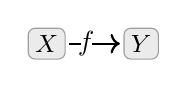
\begin{tikzpicture}[center base]
	\node[dpadinline] (X) at (0,0) {$X$};
	\node[dpadinline] (Y) at (1.2,0){\small$Y$};
 	\draw[arr1,->] (X) -- node[fill=white, fill opacity=1, pos=0.35, inner sep=-1pt]{$f$} (Y);
\end{tikzpicture}\,.
% This presentation is looks slightly different from the original presentation in \cite{richardson2020probabilistic}, but is equivalent.
% This presentation is equivalent to one in which edge sources and targets are both \emph{sets} of variables.
\Cref{defn:pdg} is equivalent to one in which edge sources and targets are both \emph{sets} of variables.
% \cite{richardson2020probabilistic}.
This allows us to indicate joint dependence with multi-tailed arrows, joint distributions with multi-headed arrows,
and unconditional distributions with nothing at the tail.
For instance, we draw
% For instance, we will draw
%oli2:
%
% \\
\\[-0.0ex]
% \[
	% p(Y|X,Z)~
	% \text{as}~
	% p(Y|X,Z)~\text{as}~
	$p(Y|X,Z)$ as
	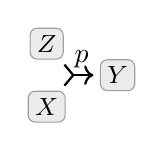
\begin{tikzpicture}[center base]
		\node[dpadinline] (Y) at (0.9,0) {$Y$};
		\node[dpadinline] (X) at (0,-0.4) {$X$};
		\node[dpadinline] (Z) at (0, 0.4) {$Z$};
		\mergearr[arr2] XZY
		\node[above right=-1pt and -3pt of center-XZY] {$p$};
	\end{tikzpicture}\,,
    % ~~\text{and $q(Y)$ as }~~
	% \begin{tikzpicture}[center base]
	% 	\node[dpad0] (Y) at (1,0) {$Y$};
	% 	\draw[arr2, <-] (Y) -- node[left,inner sep=2pt]{$q$} ++(0,1);
	% \end{tikzpicture}~.
    % ~\text{and $q(A,B)$ as }~
    and $q(A,B)$ as
	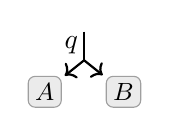
\begin{tikzpicture}[center base]
		\node[dpadinline] (A) at (0,0) {$A$};
        \node[dpadinline] (B) at (1,0) {$B$};
        \coordinate (above) at (0.5,0.8);
        \coordinate (center) at (0.5,0.4);
		% \draw[arr2, <-] (Y) -- node[left,inner sep=2pt]{$q$} ++(0,1);
        \cunmergearr[arr1] {above}{A}{B}{center}
        \node[above left=0pt and 0pt of center,inner sep=2pt]{$q$};
	\end{tikzpicture}\,.
%
%joe1*: you need to SLOW DOWN here and reimnd the reader what these
%pictures are saying.  They do not have access to your mind
%oli1: added one more example to ease into it.
%oli2:
%
% An unconditional distribution $p(X)$ can be given by associating it to a hyper-edge $\emptyset \to \{X\}$, or directly by \cref{defn:pdg} by taking its source to be a ``variable'' that can only take on one possible value.
% We will not make much use of $\alpha$ here, so $\mat p$ and $\beta$ are the most important
%
% By default, all cpds are associated with confidence $\beta = 1$.
%%joe1: do we actually ever do it?
%%oli1:
%% only when applying Lemma 1, which I have now rewowrded so this is unnecessary.
% A cpd $p$ can be regarded as a PDG with a single edge (with $\bp[p] =
% p$, and  $\alpha_p=0$ and $\beta_p = 1$ by default), and sometimes we
% make this conversion implicitly.
% p$, and  $\alpha_p=0$ and $\beta_p = 1$;   we sometimes do so.
%% union is not really used.
% The union of $\dg M$ and $\dg M'$ is denoted by $\dg M + \dg M'$.
% To emphasize that an edge is degenerate (a function), we will draw it
To emphasize that a cpd $f(Y|X)$ is degenerate
(a function $f:X\to Y$),
% (a function),
we will draw it with two heads, as in:
%joe1*: Draw an example!
%oli1: done.
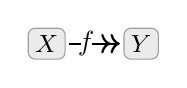
\begin{tikzpicture}[center base]
	\node[dpad0, inner sep=2.5pt, rounded corners=2.5pt] (X) at (0,0) {\small$X$};
	\node[dpad0, inner sep=2.5pt, rounded corners=2.5pt] (Y) at (1.2,0){\small$Y$};
 	\draw[arr1,->>] (X) -- node[fill=white, fill opacity=1, pos=0.35, inner sep=-1pt]{$f$} (Y);
\end{tikzpicture}\,.
%oli2: reorder
% We identify an event $X\!\!=\!x$ with the degenerate distribution on $X$ that places all mass on $x$, and hence may be associated to an edge.
%joe1
%Furthermore, as is unambiguous to shorten this event to simply $x$, as
%the label of an edge.
%oli1:
% We occasionally write $x$ rather than $X=x$ as the label of the edge.
% We will label such an edge simply by `$x$'.
% We label such an edge simply as `$x$'.
We identify an event $X\!\!=\!x$ with
% the degenerate distribution $\delta_x(X)$ that places all mass on $x$;
the degenerate unconditional distribution $\delta_x(X)$ that places all mass on $x$;
hence it may be associated to an edge and drawn simply as
% We label such an edge simply as `$x$'.
\begin{tikzpicture}[center base]
	% \node[dpad0, inner sep=2pt, rounded corners=2pt] (Y) {\small$X$};
	\node[dpadinline] (Y) {\small$X$};
 	\draw[arr1,<<-] (X) --
		% node[fill=white, fill opacity=1, pos=0.60, inner sep=1pt]{$x$} +(-1,0);
		node[above, pos=0.60, inner sep=1pt]{$x$} +(-1,0);
\end{tikzpicture}\,.
%oli: REMOVED
% By default, edges have $\beta = 1$,
% which is just a convenient choice of units---what’s important are the magnitudes of $\beta$ relative to each other (and to $\gamma$, for $\gamma$-inconsistency).
To specify a confidence $\beta \ne 1$,
%
%joe1*: why a lighter color?  This makes it harder to read, and does
%not help (at least, not me) in any way.  I strongly recommend that
%you don't use a lighter color
%oli1: the lighter color really reduces visual clutter for me.
%
% we put it in a parentheses
% and a lighter color nearby the edge, as in:
we place the value near the edge, lightly colored and parenthesized, as in:
% % By default, all cpds are associated with confidence $\beta = 1$.
% A cpd $p$ can be regarded as a PDG with a single edge (with $\bp[p] = p$, and  $\alpha_p=0$ and $\beta_p = 1$ by default), and sometimes we make this conversion implicitly.
% %% union is not really used.
% % The union of $\dg M$ and $\dg M'$ is denoted by $\dg M + \dg M'$.
% We identify an event $X=x$ with with the degenerate distribution on $X$ that places all mass on $x$, and hence may be associated to an edge.
% Furthermore, as is unambiguous to shorten this event to simply $x$, as the label of an edge.
% To emphasize that an edge is degenerate (a function), we will draw it with two heads.
% To specify a confidence $\beta \ne 1$, we put it in a parentheses and a lighter color nearby the edge, as in
% $p ~^{\color{gray}{(\beta\colon0.7)}}$, or
% $p^{\color{gray}(\beta)}$ as a compressed form of
% of $p^{\color{gray}{(\beta:\beta)}}$.
\!\!\!\!
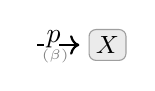
\begin{tikzpicture}[center base]
	\node[dpad0, inner sep=2.5pt, rounded corners=2.5pt](X){\small $X$};
    \draw[arr, <-]  (X) --
        node[above,pos=0.62, inner sep=1pt, outer sep=-2pt, fill=white]{$p\!$}
        node[below,pos=0.55, inner sep=0, outer sep=1.5pt]{${\scriptscriptstyle\color{gray}(\beta)}$}
         ++(-1,0);
\end{tikzpicture}\,,
%
%joe1*: I think that this is a bad idea.  Help the reader and use
%\beta \to \inftyh.  You may be used to your notation, but the typical
%reader will absolutely not be.
% Finally, we write ${\scriptstyle\color{gray}(\infty)}$ to denote the limit of high confidence ($\beta \to \infty$). % $\alpha$.
% and write ${\scriptstyle\color{gray}(\infty)}$ to denote the limit of high confidence ($\beta\!\to\! \infty$). % $\alpha$.
and we write ${\scriptstyle\color{gray}(\infty)}$ for the limit of high confidence ($\beta\!\to\! \infty$). % $\alpha$.
% We will not
% To inciate the limit of high confidence on a cpd $p$, we write an exclamation point, as in: \tikz[baseline=0.9] \draw[arr, <-] node[dpad0](X){$X$} (X) -- node[below,pos=0.6, inner sep=2pt]{$p!$} ++(-1,0);.
 % ($\beta_p \to \infty$)


% \subsection{Monotonicity of Inconsistency}
%oli2: no more subsection
% \subsection*{Monotonicity of Inconsistency}


% It is easy to show that adding edges, or increasing their confidences, cannot decrease the inconsistency of a PDG.
Intuitively, believing more things can't make you any less inconsistent.
\Cref{lemma!}
% our workhorse lemma for deriving relationships between loss functions, captures this formally: adding edges, or increasing confidences, cannot decrease the inconsistency of a PDG.
captures this formally: adding cpds or increasing confidences cannot decrease a PDG's inconsistency.

\newsavebox\olibox
\sbox\olibox{$\aar{\;\cdot\;}$}
\begin{linked}[{Monotonicity of
		% $\langle\!\\langle\,\cdot\,\rangle\!\rangle$}]
		\usebox\olibox}]
		{lemma}{!}
	\label{lemma!}
 	% For all pdgs $\dg M$ and $\dg M'$, with respective confidence vectors $\beta$ and $\beta'$,
	% and all $\gamma > 0$,
	% we have that
	% If $\dg M$ and $\dg M'$ are PDGs differ only in their edges (respectively $\Ed$ and $\Ed'$) and confidences ($\boldsymbol\beta$ and $\boldsymbol\beta'$), then for all $\gamma >0$, we have that:
%
	% \begin{enumerate}[label={\arabic*.}]
	% 	%joe1: the + notation is undefined
	% 	% \item  $\aar{\dg M + \dg M'}_\gamma \ge \aar{\dg M}_\gamma$.
	% 	\item  If $\Ed \subseteq \Ed'$, then $\aar{\dg M}_\gamma \le \aar{\dg M'}_\gamma$.
	% 	%oli1: another possibility
	% 	% \item  $\aar{\dg M + \dg M'}_\gamma \ge \aar{\dg M}_\gamma$,
	% 		%where $\dg M + \dg M'$ is the union of $\dg M$ and $\dg M'$.
	% 	\item If
    %         % and $\beta \succeq \beta'$ (that is, $\beta_L \ge \beta'_L$ for all $L \in \Ed$), then $\aar{\dg M} \ge \aar{\dg M'}$.
	% 		$\Ed = \Ed'$ and
    %         $\beta_L \le \beta'_L$ for all $L \in \Ed$, then $\aar{\dg M} \le \aar{\dg M'}$.
	% \end{enumerate}
	%%%%%%%%%
	% If $\dg M$ and $\dg M'$ are PDGs differ only in their edges (respectively $\Ed$ and $\Ed'$) and confidences ($\boldsymbol\beta$ and $\boldsymbol\beta'$), then for all $\gamma >0$, we have that:
	%%%%%%%%%
	Suppose PDGs $\dg M$ and $\dg M'$ differ only in their edges (resp. $\Ed$ and $\Ed'$) and confidences (resp. $\boldsymbol\beta$ and $\boldsymbol\beta'$).
	If $\Ed \subseteq \Ed'$ and
		$\beta_L \le \beta'_L$ for all $L \in \Ed$, then $\aar{\dg M}_{\gamma} \le \aar{\dg M'}_{\gamma}$ for all $\gamma$.%
	\footnote{All proofs can be found in \cref{appendix:proofs}.}
	% If $\dg M = (\N, \Ed, \V, \mathbf p, \boldsymbol\alpha, \boldsymbol\beta)$ is PDG, and  $\dg M' = (\N, \Ed', \V, \mathbf p, \boldsymbol\alpha, \boldsymbol\beta')$ for some $\Ed' \subseteq \Ed$ and
	% $\boldsymbol\beta'$ such that $\beta_L' \le \beta_L$ for all $L \in \Ed'$, then $\aar{\dg M}_{\gamma} \le \aar{\dg M'}_{\gamma}$ for all $\gamma$.
\end{linked}
\vspace{-1ex}

This tool is sufficient to derive many interesting relationships between loss functions.
% \section{SIMPLE INFORMATION-THEORETIC OBJECTIVES AS INCONSISTENCY}
% \section{INFORMATION-THEORETIC EXPRESSIONS AS INCONSISTENCY}
% \section{SURPRISE AS INCONSISTENCY}
% \section{NEGATIVE LOG LIKELIHOOD AS INCONSISTENCY}
\section{STANDARD METRICS AS INCONSISTENCIES}

% \def\xsamp{{\underline{\mat x}}}
% \def\xysamp{{\underline{\mat{xy}}}}
\def\xsamp{{\mathcal D}}
\def\xysamp{{\mathcal D}}

% To illustrate how the inconsistency of a PDG can start to generate information theoretic expressions,
% Let's start with a simple example.
% We start with a simple example.
Suppose you believe that $X$ is distributed according to $p(X)$,
and also that it (certainly) equals some value $x$. These beliefs are consistent if $p(X\!\!=\!x) =\! 1$
% and become more inconsistent
but become less so
 as $p(X\!\!=\!x)$ decreases.
In fact, this inconsistency
is equal to
% equals
the
%joe1I*: there shoudl be a reference, and hyou need to discuss this to
%make it clear that it's a standard notion.
%information content (or surprise) of the event $X \!\!=\! x$,
information content  $\I_p[X\!\!=\!x] := -\log p(X\!\!=\!x)$, or \emph{surprisal} \parencite{tribus1961information}, of the event $X \!\!=\! x$,
according to $p$.%
%oli: footnote moved
\footnotemark\
% \footnote{Here we implicitly identifed $p$ with its probability mass function. One can get similar, but subtler, results for densities. See \cref{appendix:density} for details.}
In machine learning, $\I_p$ is usually called ``negative log
likelihood'', and is perhaps the most popular objective for training
generative models
%\parencite{deepgennotes}\parencite{myung2003tutorial}.%
\parencite{deepgennotes,myung2003tutorial}.%

%floating footnote.
% \footnotetext{Here we implicitly identify $p$ with its probability mass function. One can get similar, but subtler, results for densities. See \cref{appendix:density} for details.}
\footnotetext{This construction requires the event $X\!\!=\!x$ to be measurable.
  	One can get similar, but subtler, results for densities, where this is not the case; see \cref{appendix:density}.}

\begin{linked}{prop}{pdg-Ix}
	Consider a distribution $p(X)$.
	The inconsistency of the PDG comprising $p$ and $X\!\!=\!x$
	% is equal to the
	equals
	the surprisal $\I_p[X\!\!=\!x]$.
	% of the event $X\!\!=\!x$
	That is,
	\vspace{-2ex}
	% \vskip-1ex
	\[
		\I_p[X\!\!=\!x]
		% := \log \frac{1}{p(X \!\!=\! x)}
		=
		\aar[\Big] {
		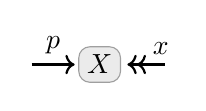
\begin{tikzpicture}[baseline=-0.7ex]
			\node[dpad0] (X) {$X$};
			\coordinate (A) at ($(X) + (-0.9,0)$);
			\draw[arr1] (A) -- node[above]{$p$}  (X);
			%
			\draw[arr2, <<-] (X) --  node[above,pos=0.8]{$x$} ++(0.9, 0);
		\end{tikzpicture}
		}.
	\]
	\vspace{-1ex}
	%oli2:
	(Recall that $\aar{\dg M}$ is the inconsistency of the P\kern-1ptD\kern-1ptG $\dg M$%
% 		;here, $\dg M = $ \begin{tikzpicture}[center base]
% 		\node[dpad0] (X) {$X$};
% 		\coordinate (A) at ($(X) + (-0.9,0)$);
% 		\draw[arr1] (A) -- node[above]{$p$}  (X);
% %
% 		\draw[arr2, <<-] (X) --  node[above,pos=0.8]{$x$} ++(0.9, 0);
% 	\end{tikzpicture}
	.%
	)
\end{linked}
%joe1*: Again, SLOW DOWN and helpe the reader by explaining what the
%PDG is saying

In some ways, this result is entirely unsurprising, given that
% PDG inconsistency
\eqref{eq:inc} is a flexible formula built out of information theoretic primitives.
%
% Even so, it is worth noting that
Even so, note that
% With a little more focus on the context and less on the algebra, perhaps \Cref{prop:pdg-Ix} becomes more curous:
% the inconsistency of the PDG containing just a distribution $p(X)$ and
% a sample $x$ happens to be the standard relationship between a
 % the inconsistency of the PDG containing just a distribution $p(X)$ and
 % a sample $x$ happens to be the standard relationship between a
% the inconsistency of believing both a distribution $p(X)$ and an event $X\!\!=\!x$
the inconsistency of believing both a distribution and an event
happens to be the standard measure of discrepency between the two%
%joe1
%distribution $p$ and sample $x$ --- and it is even known known as
% distribution $p$ and sample $x$---and it is even named after
---and is even named after
%joe1*: the notion of "cognitive dissonance" has a lot of baggage that
%comes with it (Festinger's experiments).  I doubt that most
%psychologists would associate surprise with cognitive dissonance.  I
%woujld *strongly* recommend that you don't bring it up here, unless
%you can make a much better connectin.
%``surprise'', a particular kind of cognitive dissonance.
%oli1: I'll use different words then:
% ``surprise''.
``surprise'', a particular expression of epistemic conflict.

% For this argument to be pesuasive, one needs to accept our definition of inconsistency more broadly. \Cref{prop:pdg-Ix} is a very simple special case.
% One concern is that it does not model the whole state of affairs; we train probabilstic models models with more than one sample.
Still, we have a ways to go before this amounts to any more than a curiosity.
One concern is that this picture is incomplete; we train probabilistic models with more than one sample.
What if we replace $x$ with an empirical distribution over many samples?
% The first step in the proof of \cref{prop:pdg-Ix} is no longer valid, but we can get the same effect by being extremely confident in the data distribution.
{
\def\xsamp{{\mathcal D}}
\begin{linked}{prop}{expected-surprise}
	% Given a model
    % determining a probability distribution with mass function
	If
	%joe1: what do you mean by "model" here.  Can you nsut say that p(X)
	%is a distribution on X.
	%%oli1: yes, but my audience here is people who use cross-entropy, and might not
	%% think of their generative models as probabilisty distributions without prodding. Try this:
    % $p(X)$ is a model,
    $p(X)$ is a probabilistic model of $X$,
	% and $\xsamp = \{ x_i \}_{i=1}^m$ are samples
	and $\xsamp = \{ x_i \}_{i=1}^m$ is a dataset
    with empirical distribution $\datadist\xsamp$, then
	~~~$\mathrm{CrossEntropy}(\datadist\xsamp, p) = $
    %
	\vskip-4ex
    % \begin{align*}
	\[
        % \frac{1}{m} \sum_{i=1}^m \I_p(x_i)
        \frac{1}{m} \sum_{i=1}^m \I_p[X\!\!=\!x_i]
		%&
		=
        \aar[\Big] {
		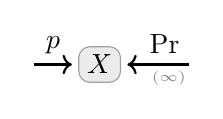
\begin{tikzpicture}[center base]
			\node[dpad0] (X) {$X$};
			\coordinate (A) at ($(X) + (-0.9,0)$);
			\draw[arr2] (A) -- node[above]{$p$}  (X);
			\draw[arr2, <-] (X) --
                node[above,pos=0.6,inner sep=2pt]{${\datadist\xsamp}$}
                node[below,pos=0.65,inner sep=2pt]
                    {${\color{gray}\scriptscriptstyle(\infty)}$}
             ++(1.2, 0);
				%\overset{\{\beta = \infty\}}
		\end{tikzpicture}
		}%_\gamma
        %
		%joe1*: putting this in gray is distracting and makes it harder to
		%read.  I see no benefit.
		%oli1: Fiiiiine, I begrudingly accept the standard
		% ~{\color{gray}+ \H(\datadist\xsamp)}.
		~{+ \H(\datadist\xsamp)}
        % \\
        % &= \mathrm{CrossEntropy}(\datadist\xsamp, p)
		.
	% \end{align*}
	\]
% 	\begin{enumerate}
% 	\item The average negative log likelihood $\ell(p; \xsamp) = - \frac{1}{m} \sum_{i=1}^m \log p(x_i)$
% 	\item The cross entropy of $p$ relative to $\datadist\xsamp$
% 	\item $\bbr{\,p\,}_\gamma(\datadist\xsamp) ~{\color{gray}~+ (1+\gamma)\H(\datadist\xsamp)}$ \\[-1.4em]
% 	% FALSE! \item $\bbr{\,p^{\{\alpha=1\}} \,}_1 (\datadist\xsamp^{\{\alpha=1\}})$
% 	\item
% 	% \item
% 	% \(\aar[\Bigg] {
% 	% 	\begin{tikzpicture}[center base]
% 	% 		\node[dpad0] (X) {$X$};
% 	% 		\coordinate (A) at ($(X) + (-1.2,0)$);
% 	% 		\draw[arr1] (A) -- node[above,pos=0.4]{$ \overset {\{\alpha = 1\}} p$}  (X);
% 	% %
% 	% 		\draw[arr2, <-] (X) --  node[above,pos=0.6]{$ \overset{\{\beta = \infty,\alpha=\gamma\}}{\datadist\xsamp}$} ++(1.5, 0);
% 	% 	\end{tikzpicture}
% 	% 	}\!\bigg._1 \)
% \end{enumerate}
\end{linked}
\begin{remark}
	%oli1:
	% Note that the entropy of the data distribution $\H(\datadist\xsamp)$
	The term $H(\datadist\xsamp)$
	%joe1: If this is your reason for putting it in gray, it's a bad one
	%does not depend on $p$, and so the final grey term is irrelevant for
	%oli1: ok. rewording since I've already given the formula.
	% does not depend on $p$, and so the $\H(\datadist\xsamp)$ term is irrelevant for finding $p$ to minimize it.
	% does not depend on $p$, and hence is irrelevant for
	is a constant depending only on the data, so is irrelevant for optimizing $p$.
	% It arises because of the implicit independence assumptions in the term
\end{remark}
}

% The PDG in  \cref{prop:expected-surprise} is quite natural.
% Aside from the certainty weights $\beta$, we've simply translated each piece of information into a cpd, and collected them together as a PDG.
% We argue that the choice of $\beta$ makes sense as well, in the standard use cases for  cross entropy / log likelihood.
% % In the current setting, we argue that the weights are also the ones we would expect.
% The cross entropy measures the expected code length per sample, when a (possibly incorrect) distribution $p$ is used to design a code, in place of the true one $\datadist\xsamp$.
% So implicitly, a modeler who chooses a cross-entropy has in some sense implicitly articulated a belief the data distribution is the ``true one'', by placing infinite certainty in $\datadist\xsamp$ than in $p$.
% If $p(X)$ represents a probabilistic model before training is complete (say, a neural network with randomly initialized weights), we would be justified in placing dramatically more trust in the data $\datadist\xsamp$ than in $p$, and so this choice seems particularly appropriate.
% % This justifies the `!'.
% Other choices of $\beta$ are natural in other contexts, and we will see in \cref{sec:statdist} that they correspond to other losses. (For instance when $\beta_p = \beta_{\datadist\xsamp} = \nicefrac12$, the result is the Bhattacharyya distance, rather than the cross entropy.)
% The only choice we've made in specifying the PDG of \cref{prop:expected-surprise} are the confidences.
Essentially the only choices we've made in specifying the PDG of \cref{prop:expected-surprise} are the confidences.
% But
But
$\mathrm{CrossEntropy}(\datadist\xsamp,p)$
% the cross entropy of $p$ with respect to $\datadist\xsamp$
is the expected code length per sample
from $\datadist\xsamp$, when using codes optimized for the (incorrect) distribution $p$.
% TODO fixme. DO I need Citation? Also, this is perhaps not the best
% citation for the claim.
% \parencite{shore1980relent}.
So implicitly, a modeler using cross-entropy has already articulated a belief the data distribution $\datadist\xsamp$ is the ``true one''.
To get the same effect from a PDG, the modeler must make this belief explicit by
% placing infinite certainty in $\datadist\xsamp$.
placing infinite confidence in $\datadist\xsamp$.
% setting the confidence $\beta$ for $\datadist\xsamp$ to $\infty$.


% We now consider an orthogonal generalization of \cref{prop:pdg-Ix}, in which the sample $x$ is only a partial observation of a joint model $p(X,Z)$.
% In this case, we might hope to recover the \emph{marginal} surprise, since $Z$ does not interact with the observation. % ---  in \cref{prop:marginal-ll}.
Now consider an orthogonal generalization of \cref{prop:pdg-Ix}, in which the sample $x$ is only a partial observation of $(x,z)$ from a joint model $p(X,Z)$.
% In this case, we get the \emph{marginal} information, as $Z$ does not interact with the observation. % ---  in \cref{prop:marginal-ll}.

\begin{linked}{prop}{marginal-ll}
	If $p(X,Z)$ is a joint distribution, then the information content of the partial observation $X=x$
	% , or the marginal negative log likelihood of $x$,
	is given by
	\vskip-4ex
	\begin{equation}
	 	% \I_p(x) = \log \frac{1}{p(x)} =
	 	\I_p[X\!\!=\!x] =
		% \log \frac{1}{p(X\!\!=\!x)} =
	    % \lim_{t \to \infty}
		 \aar[\Bigg]{
	% 	  \Inc\left(
			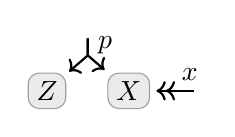
\begin{tikzpicture}[center base]
				\node[dpad0] (Z) {$Z$};
				\node[dpad0,right=.5 of Z] (X) {$X$};
				\coordinate (A) at ($ (X)!.5!(Z) + (0,0.7)$);
				\draw[arr1] (A) -- node[right]{$ p$} ++(0,-0.25) -- (X);
				\draw[arr1] (A) -- ++(0,-0.25) -- (Z);
	%
				\draw[arr2, <<-] (X) --  node[above,pos=0.8]{$ x$} ++(0.9, 0);
	% 			\draw[arr2, <-] (Z) -- node[above,pos=0.6]{$ q^{\{\beta =\infty\}}$} ++(-0.9, 0);%
				% \ar[r,"p"] \& Z \ar[r,"p", bend left] \& X \ar[l,"q", bend left] \& \ar[l, two heads, "x"']
			\end{tikzpicture}
			}.
			\label{eq:mll}
	\end{equation}
\end{linked}

Intuitively, the inconsistency of the PDG on the
right side of \eqref{eq:mll} is localized to $X$, where the observation $x$ conflicts with $p(X)$; other variables don't make a difference.
% The natural generalization with both partial observations and multiple samples also holds; we defer treatment to the appendix.
The multi-sample partial-observation generalization also holds; see \cref{appendix:more-crossent}.
% Just as \cref{prop:expected-surprise} generalizes \cref{prop:pdg-Ix}, there is
% a multi-sample analog of analog of \Cref{prop:marginal-ll} .
% Furthermore, $p$ is the qualitative model we have in mind, and so we set $\alpha_p = 1$
 % by considering more than one sample at once,



% So far we have been considering models of a distribution $p(X)$ that correspond to generative models, or an unsupervised setting.
% So far we have considered models of an unconditional distribution $p(X)$.
% Because one can use such a model to generate samples, such models are called \emph{generative}, and their training process is called \emph{unsupervised} learning.
So far we have considered models of an unconditional distribution $p(X)$.
Because they are unconditional, such models must describe how to generate a complete sample $X$ without input, and so are called \emph{generative}; the process of training them is called \emph{unsupervised} learning \parencite{elts_stat_learn2009}.
% Contrast this with the (more common) \emph{supervised} setting, in which we train \emph{discriminative} models to predict $Y$ from $X$, from labeled samples $\{(x_i,y_i)\}_i$.
In the (more common) \emph{supervised} setting, we train \emph{discriminative} models to predict $Y$ from $X$, via labeled samples $\{(x_i,y_i)\}_i$.
There, cross entropy loss is perhaps even more dominant---and it is essentially the inconsistency of a PDG consisting of the predictor $h(Y|X)$ together with high-confidence data.
{\def\xysamp{{\mathcal D}}
\begin{linked}[Cross Entropy, Supervised]
		{prop}{supervised-cross-entropy}
	% Consider a probabilistic model $f$ with mass function $f(Y \mid X)$. The inconsistency of the PDG containing $f$ and the empirical distribution $\datadist\xysamp$ of samples $\xysamp$ is equal to the negative log-liklihood (cross-entropy) loss, plus the empirical uncertainty in $Y$ given $X$ (a constant independent of $f$). That is,
    % Consider a probabilistic predictor $f(Y|X)$. The
	The inconsistency of the PDG comprising a probabilistic predictor $h(Y|X)$,
	and a high-confidence empirical
	%%joe1: is this standard notation for a set of samples?  I don't believe that
	%%I've seen it before.  If it's not standard, you have to example it better
	%    distribution $\datadist\xysamp$ of samples $\xysamp$ is equal to
	%%oli1: Not really. I was hesitant to use sets because samples could repeat, but it's
	%%	kind of irrelevant. I'll expand it in the standard way
    % distribution $\datadist\xysamp$ of a set $\xysamp$ of samples is equal to
    distribution $\datadist\xysamp$ of a dataset $\xysamp = \{(x_i, y_i)\}_{i=1}^{m}$
	% is equal to
	equals
    the cross-entropy loss (minus the empirical uncertainty in $Y$
    given $X$, a constant depending only on $\xysamp$). That is,
	\[ \aar**{
		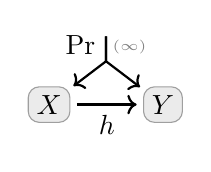
\begin{tikzpicture}[center base]
			\node[dpad0] (Y) {$Y$};
			\node[dpad0,left=.9 of Y] (X) {$X$};
			\coordinate (A) at ($ (X)!.5!(Y) + (0,0.9)$);
			%joe1*: you're back to using hte exclamation point notation, which you
			%never defined.  I *strongly* suggest that you get rid of it.  Pity
			%the poor reader!
			%oli1: oops. Missed this one.
			\draw[arr1] (A) --
				% node[right]{$\datadist\xysamp!$}
				node[left,inner sep=3pt]{$\datadist\xysamp$}
				node[right,inner sep=2pt]{${\color{gray}\scriptscriptstyle(\infty)}$}
				++(0,-0.35) -- (X);
			\draw[arr1] (A) -- ++(0,-0.35) -- (Y);
			\draw[arr2, ->] (X) --  node[below,pos=0.5]{$h$} (Y);
		\end{tikzpicture}}
        \begin{aligned}
			%oli1: This should be clearer also.
            % \frac1{|\xysamp|}\sum_{(x,y) \in \xysamp} \left[ \log \frac1{f(y \mid x)}\right]&\\
            = \frac1{m}\sum_{i=1}^m \log \frac1{h(y_i\,|\, x_i)}&\\
             - \H_{\datadist\xysamp}(Y | X)&.
        \end{aligned}
	\]
\end{linked}
}
% Once again, we get the standard loss function simply by allowing the modeler to articulate their beliefs.


% \begin{remark} \label{remark:continuous}
% % \cref{prop:pdg-Ix,prop:expected-surprise,prop:marginal-ll,prop:pdg-loglikelihood,prop:supervised-cross-entropy} all require the probability to have a mass function, rather than a density function, which implicitly restricts us to discrete variables.
% % \cref{prop:pdg-Ix,prop:expected-surprise,prop:marginal-ll,prop:pdg-loglikelihood,prop:supervised-cross-entropy}
% Many of our results require the distribution to be represented with a mass function (not a density function (pdf)).
% %joe1*: We've never talked about the inconsistency of a continuous
% %distribution.  If it's always infinite, this suggests that whatever
% %definition you have in mind is not good.  I would strongly suggest
% %that you deal with onoly discrete distributions here.  If you venture
% %into continuous distributions, you *must* explain inconsistency for
% %them better, and motivate it.   You can instead just talk about
% %approximating the continuous distrbution by a discrete
% %distribution. or perhaps a distribution that takes on only finitely
% %many values.
% %joe1*: I fell off the cliff in the next few sentences.  I strongly
% %suggest you cut them (which you can do if you say that you're just
% %considering discrete distributions.
% This is not just a quirk of the PDG formalism.
% A PDG containg both pdf and a finitely supported distribution on the same variable
% will typically have infinite inconsistency.
%
% % of the standard objectives.
% The analog of surprisal for a density $p(X)$ is problematic because probability density is not dimensionless (like probability mass), but rather has inverse $X$-units (e.g., probability per meter), so depends on an arbitrary choice of scale (the pdf for probability per meter and per centimeter will yield different numbers).
% %
% That said, a rescaling ultimately only adds a constant.
% % Similarly, any approximation of a density $p(X)$ with a discretization $\tilde p_k(X)$ where $k$ discretization size, differs only
% Moreover, refining the discretization size $k$ of a discretized approximation $\tilde p_k(X)$ also contributes a constant that depends only on $k$.
%     % \cref{prop:pdg-Ix,prop:expected-surprise,prop:marginal-ll,prop:pdg-loglikelihood,prop:supervised-cross-entropy}
% % only in a constant that depends only on $k$.
% % But this constant is irrelevant for optimization, justifying the use of the continuous analogs (such as $- \log p(x)$ for a pdf $p(x)$) as loss functions.
% Such constants are irrelevant for optimization, justifying the use of the continuous analogs as loss functions.
% %TODO Verify that this is dealt with in an accurate way.
% \end{remark}

%oli2: remove subsection
% \subsection{Simple Performance Metrics as Inconsistencies}

% There are also simple scoring metrics used to evaluate the performance of systems on datasets, such as the accuracy of a classifier, or the mean-squared error of a regressor. These too naturally arise as inconsistencies.
%oli3: or -> and
% Simple evaluation metrics, such as the accuracy of a classifier, or the mean squared error of a regressor, also arise naturally as inconsistencies.
Simple evaluation metrics, such as the accuracy of a classifier, and the mean squared error of a regressor, also arise naturally as inconsistencies.

\begin{linked}[Log Accuracy as Inconsistency]
		{prop}{accuracy}
	% If $h: X \to Y$ is a predictor for an input space $X$ and label space $Y$, and $f: X \to Y$ generates the correct labels, then the inconsistency of believing $f$ and $h$ (with any degree of confidence), and also that inputs are distributed according to $D(X)$, equals the information content of learning that $f(X) = h(X)$ according to $D$ (which is the log accuracy of the predictor $h$) times the confidence in $D$. That is,
	%joe1: You've been writing p(X).  Why suddenly switch to D(x)
	%    Consider $D(X)$ over inputs $X$, and functions $f,h : X \to Y$,
	%oli1: ... because this was more the anlog of $\Pr$, but I didn't want to insist on
	% an emperical distribution over samples. I think maybe just $\Pr$ with no subscript
	% is clearer, but it makes me slightly unhappy because then $\Pr$ isn't just a function
	% from models to probability distributions anymore.
	%TODO
    % Consider a distribution $D(X)$ over inputs $X$, and functions $f,h
    % : X \to Y$,
    %             where $h$ is a predictor and $f$ generates the true labels. The
    % inconsistency of believing all three is
	% the log accuracy of $h$. That is,
    Consider functions $f,h : X \!\to\! Y$ from inputs to labels, where $h$ is a predictor and $f$ generates the true labels.
    The inconsistency of believing $f$ and $h$ (with any confidences), and a distribution $D(X)$ with confidence $\beta$, is
	$\beta$ times
	% Consider also a distribution $D(X)$
	% The inconsistency of believing all three is
	the log accuracy of $h$. That is,
	\vskip-4ex

	\begin{equation}\label{eq:accuracy-pdg}
		\aar*{\!\!\!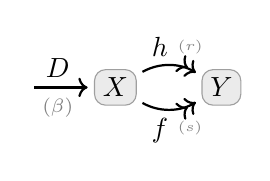
\begin{tikzpicture}[center base]
				\node[dpad0] (Y) {$Y$};
				\node[dpad0,left=0.8 of Y] (X) {$X$};
				%
				\draw[arr2, ->>] (X) to[bend left]
					node[pos=0.45,above right=4pt,inner sep=1pt]
						{{\color{gray}$\scriptscriptstyle(r)$}}
					node[pos=0.35, above]{$h$} (Y);
				\draw[arr2, ->>] (X) to[bend right]
					node[pos=0.45,below right=4pt,inner sep=1pt]
						{{\color{gray}$\scriptscriptstyle(s)$}}
					node[pos=0.35, below]{$f$} (Y);
				\draw[arr2, <-] (X) to
                    node[pos=0.55, anchor=south west, above]
					% {$\overset{(\beta)}D$} +(-1.1, 0);
					% {$D^{\color{gray}(\beta)}$}
                    {$D$}
                    node[pos=0.55, anchor=south west, below]
                    {{\color{gray}$\scriptstyle(\beta)$}}
                    +(-1.1, 0);
			\end{tikzpicture}\!}
        \begin{aligned}
		% &=  - \beta\,\log \Big( \mathrm{accuracy}_{f,D} (h) \Big) \\
		\!&=  - \beta\,\log \Pr_{x \sim D}(f(x)\!=\!h(x))  \\
		&\quad= \beta\, \I_D [f = h]. %\\[7ex]
        \end{aligned}
	\end{equation}
\end{linked}
% \vspace{-1ex}
\vskip-2.5ex
%joe1*: you need to give a reference for all this, and to discuss
%accuracy and what it's capturing *before* you state the theorem.
%DONE
% It is common to think of accuracy as a property of a hypothesis $h$
% (with some dependence on the true labeling function $f$ and the data distribution $d$), even though it is symmetric in $f$ and $g$%
One often speaks of the accuracy of a hypothesis $h$, leaving the true labels $f$ and empirical distribution $D$ implicit.
%, even though its expression is symmetric in $f$ and $h$%
%oli2: unnecessary
%, in part because we change the predictor more than the labels.
%.
% The correspondence of \Cref{prop:accuracy} graphically depicts this symmmetry, and also a more subtle phenomenon: a particularly strong dependence on the distribution of inputs.
% In fact, the inconsistency of the PDG in \eqref{eq:accuracy-pdg} is scaled by the confidence of $D$, but does not depend at all on the confidences in $h$ or $f$.
% \Cref{prop:accuracy} graphically depicts this symmmetry, a more subtle phenomenon: a particularly strong dependence on the distribution of inputs.
% Yet in some sense,
% Yet this result suggests that there is a sense in which
% Yet there is a sense in which
Yet \Cref{prop:accuracy} suggests that there is a sense in which
$D(X)$ plays the primary role: the inconsistency in \eqref{eq:accuracy-pdg} is scaled by the confidence in $D$, and does not depend on the confidences in $h$ or $f$.
%
%\DONE[needs a lot of cleanup]
% Why should this be the case? The deterministic nature of $f$ and $h$ encodes extreme confidence (to anthropomorphise: $f$ thinks it impossible that $Y \ne f(X)$, because that event has probability zero).
% Why is this the case? Because $f$ is deterministic, codes optimized for it cannot express a sample $(x,y)$ such that $y \ne f(x)$, and so a joint distribution $\mu$ incurs infinite cost if $\mu(x,y) > 0$.
Why should this be this the case?
% No matter how 
% Because $f$ is deterministic, using codes optimized for $f$ to express $(x,y)$ such that $y \ne f(x)$ is not just expensive, it is impossible---no matter how much inefficiency we're willing to tolerate. 
Expressing $(x,y)$ such that $y \ne f(x)$ with codes optimized for $f$ is not just inefficient, but impossible.
The same is true for $h$, so
% The same is true for $h$, so the confidences of $f$ and $h$ don't matter, and
% So the only way to selectively choose samples to make things consistent is to select a distribution $\mu$ on \emph{inputs}, so that it is always the case that $f(x) = h(x)$.
we can only consider $\mu$
such that $\mu(f \!=\! h) \!=\! 1$.
% , a restriction which in turn generates inconsistency equal to $D$'s surprisal that $h$ is correct.
% to restrict to $\mu(X)$ for which $\mu(f = h = Y) = 1$.
% This restriction
% in turn generates inconsistency with $D(X)$.
% In other words, the only way to reduce inconsistency smoothly is to throw out samples that don't fit, not to change the hypothesis $h$.
% In other words, the optimal distribution $\mu^*$ throws out incorrect samples, so its conditional $\mu^*(Y|x)$ is undefined unless $h(x)$ is already correct.
In other words, the only way to form a joint distribution \emph{at all} compatible with both the predictor $h$ and the labels $f$, is to throw out samples that the predictor gets wrong---and the cost of throwing out samples scales with your confidence in $D$, not in $h$.
% to change $h(Y|X)$.
% But it is the direction that we want to pull $\Pr(Y| X)$ that
% informs how we should update our predictor $h(Y\,|\,X)$, which
%joe1*: Where did non-differentiability come from?  This is totally
%out of the blue.    You should fget rid of it.
%DONE
% reflects the non-differentiability of the accuracy (or zero-one loss)
% This illustrates why accuracy is a poor loss function for training a model $h$.
% This illustrates why accuracy (the 0-1 loss) gives no gradient information for training $h$.
% This illustrates why accuracy gives no gradient information for training $h$.
This illustrates why accuracy gives no gradient information for training $h$.
% (only for $D$).
% with respect to $h$.
% Note that this is
It is worth noting that this is precisely
% This is precisely
% the opposite of how we captured cross entropy in \cref{prop:supervised-cross-entropy}:
the opposite of what happened in \cref{prop:supervised-cross-entropy}: there we were unwilling to budge on the input distribution, and 
% the optimal distribution told us how to modify $h$.
the inconsistency scaled with the confidence in $h$.
%

% Observe how even properties of these simple metrics---the lack of gradient information, and relationships to
%  	other metrics%
% 	% ---are clarified by focusing on the model.
% 	---are clarified by an underlying model.
 % We reiterate that the  . Observe that the model
 % Each of our these insights
Observe how even properties of these simple metrics---%
relationships with one another and features of gradients%
	% ---are clarified by focusing on the model.
	% ---are clarified by an underlying model.
	---can be clarified by an underlying model.


% \begin{prop}[Cosine similarity as inconsistency]
% 	\todo
% \end{prop}
%% Confusion matrix costs
% \begin{prop}
% 	\[
% 	\]
% \end{prop}




% When $Y$ is continuous rather than discrete, the estimator is referred
% to as a regressor instead of a classifier, and the newfound topology
% $Y$ suggests that some mistakes are worse than others---that we
% might want to treat a small deviation from the correct value of $Y$.
When $Y \cong \mathbb R^n$, an estimator $h(Y|X)$ is referred
to as a regressor instead of a classifier.
In this setting, most answers are incorrect, but some more so than others.
A common way of measuring incorrectness is with mean squared error (MSE):
$\Ex |f(X)-Y|^2$.
%joe1*: this is a nonsequitur from the egnning of the paragraph.
%Also, what does it mean that f and h "control" the mean of a
%Gaussian?  Do you mean that they determine some parameters of the
%Gaussian?  If so, you should say that.
%oli1: slight reword so no "control" anymore.
% Perhaps the most common way of measuring this deviation is with mean
% square error, which corresponds to the inconsistency of believing that
MSE is also the inconsistency of believing that
%joe1
%$f$ and $h$ control the mean of a unit-variance gaussian.
% $f$ and $h$ control the mean of a unit Gaussian.
%oli1: fixed
the labels and predictor have Gaussian noise---%
often a reasonable assumption because of the central limit theorem.

\begin{linked}[MSE as Inconsistency]{prop}{MSE}% \label{coro:MSE}
	\begin{align*}
		% \aar**{\begin{tikzpicture}[center base]
		% 	\node[dpad0] (Y) {$Y$};
		% 	\node[dpad0,left=1.1 of Y] (X) {$X$};
		% 	%
		% 	\draw[arr2, ->] (X) to[bend left]
		% 		node[pos=0.5, above] {$\mathcal N(f(x), 1)$} (Y);
		% 	\draw[arr2, ->] (X) to[bend right] node[pos=0.5, below]{$\mathcal N(g(x), 1)$} (Y);
		% 	\draw[arr2, <-] (X) to node[pos=0.6, above]{$D!$} +(-1.1, 0);
		% \end{tikzpicture}}
		% &=
		\aar**{\!\!\!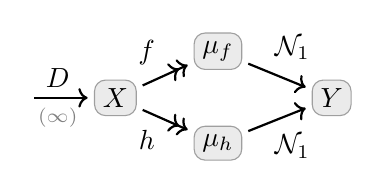
\begin{tikzpicture}[center base]
			\node[dpad0] (Y) {$Y$};
			\node[dpad0,left=2.2 of Y] (X) {$X$};
			\node[dpad0,above right=0.1 and 0.7 of X] (mf) {$\mu_f$};
			\node[dpad0,below right=0.1 and 0.7 of X] (mh) {$\mu_h$};
			%
			\draw[arr2, ->>] (X) to[bend left=0]
				node[pos=0.5, above left=0] {$f$} (mf);
			\draw[arr2, ->>] (X) to[bend right=0]
				node[pos=0.5, below left=0] {$h$} (mh);
			%
			% \draw[arr2, <-] (X) to node[pos=0.6, above]{$D!$} +(-1.1, 0);
			\draw[arr2, <-] (X) to
                node[pos=0.55, above] {$D$}
                node[pos=0.55, below]
                {{\color{gray}$\scriptstyle(\infty)$}}
                +(-1.1, 0);
			%
			\draw[arr2, ->] (mh) to[bend right=0]
				node[pos=0.3, below right=0] {$\mathcal N_1$} (Y);
			\draw[arr2, ->] (mf) to[bend left=0]
				node[pos=0.3, above right=0]{$\mathcal N_1$} (Y);
			% \draw[arr2, <-] (X) to node[pos=0.6, above]{$D$} +(-1.1, 0);
		\end{tikzpicture}\!\!}
		\begin{aligned}
        = \frac12\Ex\nolimits_D \!\big| f(X) - h(X) \big|^2 \\
		 =: \mathrm{MSE}_D( f, h )\,,\;
        \end{aligned}
        %\numberthis\label{eq:mse}
	\end{align*}
	where
    % $\mathcal N_1 = \mathcal N(-,1)$
    % $\mathcal N_1$
    $\mathcal N_1(Y|\,\mu)$
    % is the unit normal distribution with the given mean.
	% is the unit-variance normal distribution with the given mean.
	% is the unit normal distribution with given mean.
	% is a unit Gaussian with the given mean.
	% is a unit Gaussian with mean $\mu$.
	is a unit Gaussian on $Y$ with mean $\mu$.
	% is a Gaussian with mean $\mu$ and variance $1$. %% TOO LONG
\end{linked}

%oli3: added "univariate".
% In the appendix, we treat general
In the appendix, we treat general univariate
Gaussian predictors, with arbitrary variances and confidences.

% MODEL-BASED APPROACH.
% Observe how  follows clearly once we have specified a model.
% We reiterate that the  . Observe that the model
% Each of our these insights


%%%%%%%%%%%%%%%%%%%%%%%%%%%%%%%%%%%%%%%%%%
% The fact that $\mathrm{QM}(a, b) > \mathrm{GM}(a,b)$ for $a, b >0$ has been used to movivate a metric  between different power means is sometimes used to measure the
% \eqref{eq:2gaussians} and  gives
% \begin{equation*}
% \aar**{\begin{tikzpicture}[center base]
% 	\node[dpad0] (Y) {$Y$};
% 	%
% 	% \draw[arr2, ->] (X) to[bend left]
% 	% 	node[pos=0.5, above] {$\mathcal N(0, s(x))$} (Y);
% 	% \draw[arr2, ->] (X) to[bend right] node[pos=0.5, below]{$\mathcal N(0, t(x))$} (Y);
% 	\draw[arr2, <-] (Y) to node[pos=0.6, above]{$\mathcal N(0, \sigma_1)$} +(-1.4, 0);
% 	\draw[arr2, <-] (Y) to node[pos=0.6, above]{$\mathcal N(0, \sigma_2)$} +(1.4, 0);
% \end{tikzpicture}}
% =  \log
% 	 \frac
% 	 {\mathrm {QM}(\sigma_1,\sigma_2)}
% 	 {\mathrm {GM}(\sigma_1,\sigma_2)}
% \end{equation*}




% % The results in this section may not teach us very much that we did not know before, but
% Although the results in this section are not particularly useful on their own,
% they do display at a surprisingly strong tie between the standard metrics used to train probabilistic models, and the inconsistency of a corresponding PDG ---
% we have seen that (marginal) log likelihood, cross entropy, and log accuracy all arise naturally as inconsistencies of the appropriate PDGs.

%%%%%%%%%%%%%%%%%%%%%%%%%%%%%%%%%%%%%%%%%%%%%%%
\section{REGULARIZERS AND PRIORS}
\label{sec:regularizers}
Regularizers are extra terms added to loss funtions, which provide a source of inductive bias towards simple model parameters.
There is a well-known correspondence between using a regularizer and
doing maximum \emph{a posteriori} inference with a prior,%
% \footnote{A more detailed account can be found in the appendix.}
\footnote{A full account can be found in the appendix.}
% \parencite{williams1995bayesian,rennie2003l2,probinterpblogpost,mitcourse}.
% \parencite{williams1995bayesian,rennie2003l2}.
% In brief, since $\mathrm{posterior} \propto \mahtrm{likelihood} \cdo \mathrm{evidence}$,
% optimizing the log posterior
%joe1*: in what sense do they correspond?  This seems very
%mysterious.  Also, you need to tie this section in better to the rest
%of hte paper.
%oli1: I think I've done this a little better now.
in which L2 regularization corresponds to a Gaussian prior
\parencite{rennie2003l2},
% and indeed adding such a distribution to the PDG gives an extra term in the consistency, equal to the L2 regularizer.
while L1 regularization corresponds to a Laplacian prior \parencite{williams1995bayesian}.
Note that the ability to make principled modeling choices about regularizers is a primary benefit of this correspondence.
Our approach provides a new justification of it.
% This correspondence is even clearer when using PDGs. We now give our own formuulation of this result: adding a prior to the PDG results in the corresponding regularization term in the inconsistency.

\begin{linked}{prop}{regularized}
	% Suppose you believe that $Y$ is distributed according to $f_\theta(Y)$  for some parameter $\theta$, have a prior belief $p(\theta)$ over parameters, and also observe an empirical distribution $D(Y)$ which you trust. The inconsistency of also believing that the parameter is some $\theta_0$ is the \emph{regularized}-cross entropy loss, where the regularizer is $\log \frac1{p(\theta_0)}$ times your confidence in $p$.
	Suppose you have a parameterized model $p(Y|\Theta)$, a prior $q(\Theta)$, and a trusted distribution $D(Y)$. The inconsistency of
	also believing $\Theta =\theta$ is the
	% also a paremeter $\theta$ is the
	% \emph{regularized}-cross entropy loss, where the regularizer is $\log \frac1{p(\theta_0)}$ times your confidence in $p$.
 	cross entropy loss, plus the regularizer: $\log \frac1{q(\theta)}$ times your confidence in $q$.
	That is,
	%joe1*: SLOW DOWN.  Tell the reader how to interpret the PDG (you can
	%do this after the theorem statement).
	\begin{equation}\label{eq:regularize}
		\aar*{\!\!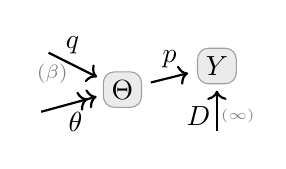
\begin{tikzpicture}[center base]
			\node[dpad0] (theta) at (0,0) {$\Theta$};
            \node[dpad0] (Y) at (1.2,0.3) {$Y$};
			% \node[dpad0, right=0.7 of theta] (Y) {$Y$};
			%
			\draw[arr] (theta) --
	 			% node[above]{$\overset{{\color{gray}(\beta_f)}}f$}
	 			% node[above]{$f^{{\color{gray}(\beta_f)}}$}
	 			node[above]{$p$}
				(Y);
			\draw[arr2, <-] (theta) --
				node[above right=-2pt and -2pt, pos=0.7] {$q$}
				node[below left=-3pt and -4pt,pos=0.6]{{$\color{gray}\scriptstyle(\beta)$}}
				++(-1.0, 0.5);
			% \draw[arr, <-] (theta) --
			% 	node[above right, pos=0.7] {$p^{{\color{gray}(\beta)}}$}
			% 	++(-1.0, 0.4);
			\draw[arr2, <<-] (theta) -- node[below,pos=0.4]{$\theta$} ++(-1.1, -0.3);
			\draw[arr2, <-] (Y) --
                node[left,pos=0.6, inner sep=2pt]{$D$}
                node[right,pos=0.6, inner sep=1pt]
                    {${\color{gray}\scriptscriptstyle(\infty)}$}
                ++(0, -0.9);
		\end{tikzpicture}\!}
		\begin{aligned}
			=\! \Ex_{y \sim D} \log \frac{1}{p(y \,|\,\theta)}
				&+ \beta \log \frac1{q(\theta)} \\[-0.2em]
	            % &\!{\color{gray}- \H(D)}
	            &\!{- \H(D)} \\[-1em]
		\end{aligned}
		% \beta_f\,
		% \Ex_{y \sim D} \left[\log \frac{1}{f(y \mid \theta_0)} \right]
        %
	\end{equation}
	%TODO Clarify why do you even need to select a little \theta?
\end{linked}

% Now, if our prior is a (discretized) unit gaussian $q(\theta) \!=\! \frac{1}{k} \exp(-\frac12 \theta^2)$ for some constant $k$,
If our prior is $q(\theta) \!=\! \frac{1}{k} \exp(-\frac12 \theta^2)$%
, a (discretized) unit gaussian%
,
then the right hand side
% then the RHS
of \eqref{eq:regularize} becomes
\[ \underbrace{\Ex\nolimits_{D}
	% \!
	% \left[
	\log \frac{1}{p(Y \,|\, \theta)}
	% \right]
	}
	_{\substack{\text{Cross entropy loss}\\(\text{data-fit cost of $\theta$})}}%(f_\theta; D)
	\; + \!\!\!\!\underbrace{~\frac\beta2 \theta_0~}_{\substack{\text{L2  regularizer}\\(\text{complexity cost of $\theta$})}} \!\!\!\!\!
	% {\color{gray!80}
	{\color{black} +
		\underbrace{\beta \log k - \H(D)}_{\text{constant in $p$ and $\theta$}}}\,, \]
which is the L2 regularized version of \cref{prop:expected-surprise}.
Moreover, the regularization strength corresponds exactly to the confidence $\beta$.
What about other priors? It is not difficult to see that if we use a (discretized) unit Laplacian prior, $q(\theta) \propto \exp(-|\theta|)$, the second term instead becomes $\beta |\theta_0|$, which is L1 regularization.
More generally, to consider a complexity measure $U(\theta)$, we need only include the Gibbs distribution $\Pr_U(\theta) \propto \exp(-U(\theta))$ into our PDG.
%% TODONE revistit %%%%% True. But helpful??
% And if we lift the requirement that $\theta$ be a point mass, the optimal distribution over $\theta$ is the posterior distribution after a Baysian update.
%
% We remark that there is nothing special about cross entropy here;
We remark that nothing here is specific to cross entropy;
%joe1*: Saying you can do it for one other proposition doesn't seem
%like convincing evidence that it's quite general
%oli1: oops.
% such a prior may be added to the pdg of \cref{prop:MSE} to instead
% regularize square loss.
% Such a priors may be added to any PDG to effectively add regularization terms.
any of the objectives we describe can be regularized in this way.

% TODO?
% ENtropy regularization is free.

%%%%%%%%%%%%%%%%%%%%%%%%%%%%%%%%%%%%%%%%%%%%%%%%%%%/%%%%%%%%%%%%%%%%%%%%%%
\section{STATISTICAL DISTANCES AS INCONSISTENCIES} \label{sec:statdist}

%%% THIS IS HERE JUST SO THAT IT RESULTS ON THE RIGHT PAGE LATER. IGNORE FOR NOW.
\begin{figure*}
	\centering
	\def\ptradius{0.07}
	\begin{tikzpicture}[xscale=1.8, yscale=1.4]\def\rotateangle{39}
		% \draw[help lines, color=gray!30, dashed] (-0.9,-1.4) grid (5.9,2.9);
		% \draw[->,thick] (-1,0)--(6,0) node[right]{$\beta_p$};
		% \draw[->,thick] (0,-1.5)--(0,3) node[above]{$\beta_q$} ;

		\draw[help lines, color=gray!30, dashed] (-1.2,-1.1) grid (5.9,2.7);
		\draw[->,thick] (-1.3,0)--(6,0) node[right]{$\beta_p$};
		\draw[->,thick] (0,-1.2)--(0,2.8) node[above]{$\beta_q$} ;

		%concave part
		% \fill[gray, fill opacity=0.2] (-1,1) -- (1.5,-1.5) -- (-1,-1.5) --cycle;
		\fill[gray, fill opacity=0.2] (-1.3,1.3) -- (1.2,-1.2) -- (-1.3,-1.2) --cycle;
		\draw[gray, opacity=0.5, thick] (-1.3,1.3) --
		node[below left=0.5em and 1.5em, anchor=north, rotate=-\rotateangle,font=\footnotesize,fill=gray!20,fill opacity=0.8, inner sep=1pt, outer sep=3pt] % at (-0.5,-0.5)
			% {Non-convex region} (1.5,-1.5);
			{Non-convex region} (1.2,-1.2);
		%axis of symmetry
		% \draw[color=orange!25, thick] (-1, -1) -- (3,3);
		% \fill[orange, opacity=0.05] (-1,-1) -- (3,3) -- (-1,3) -- cycle;
		\draw[color=gray!80!orange!45, densely dashdotted] (-1, -1) -- (3,3);
		% \draw[color=gray!80!orange!45, thick, <->] (2.8, 2.2) -- node[above right, anchor=south, rotate=-\rotateangle,font=\footnotesize,fill=white,fill opacity=0.8, inner sep=1pt, outer sep=3pt]{Axis of Symmtry}(2.2,2.8);
		\draw[color=gray!80!orange!45, thick, <->] (1.8, 1.2) -- node[above right, anchor=south, rotate=-\rotateangle,font=\footnotesize,fill=white,fill opacity=0.8, inner sep=1pt, outer sep=3pt]{\scalebox{0.8}{Axis of Symmtry}}(1.2,1.8);


		% Renyi Entropy Line
		\draw[blue!40, densely dashed, very thick, opacity=0.8]
		 	(0,1) -- node[below, align=center, pos=0.8, font=\footnotesize]{R\'enyi divergences\\for $\alpha \in (0,1)$} (5.6,1)
			(5.6,-1) -- node[above, align=center, pos=0.2, font=\footnotesize]{(negative) R\'enyi divergences\\ for $\alpha \in (1,\infty)$} (1,-1);
		%Chernoff Information Line
		\draw[red!90!blue!40, densely dashed, very thick, opacity=0.9, (-), shorten <=6pt, shorten >=6pt]
		 	(0,1) --
            node[pos=0.5,below left=3pt,anchor=north, rotate=-\rotateangle, font=\footnotesize, align=center, fill=white,fill opacity=0.8, inner sep=1pt, outer sep=2pt]
                {\scalebox{0.9}{Chernoff}}
            node[pos=0.5,below left=1.25em,anchor=north, rotate=-\rotateangle, font=\footnotesize, align=center, fill=white,fill opacity=0.8, inner sep=1pt, outer sep=2pt]{\scalebox{0.9}{Divergences}}
            (1,0);
		%alpha divergence line
		% \draw[domain=1.5:5.6, smooth, very thick, variable=\x, blue!50!green!50, opacity=0.8, densely dashed] plot ({\x}, {1/(1-1/\x)})
		\draw[domain=1.6:5.6, smooth, very thick, variable=\x, blue!50!green!50, opacity=0.8, densely dashed] plot ({\x}, {1/(1-1/\x)})
			node[rotate=-7, font=\footnotesize] at (3.9,1.55){$\alpha$-divergences};

		%%%% POINTS %%%%
		%[draw, very thick,fill=magenta!50!black]
		\fill (0.5,0.5) circle (\ptradius) node[above right, align=center,
			label={[yshift=0ex,xshift=-1ex,align=left,font=\footnotesize\color{gray!50}]right:Bhattacharya\\distance}]
			% {Bhattacharya\\distance};
			% {$\thickD^{\text{Bhattacharya}}$};
			{$\thickD_{B}(p,q)$};

		% \fill (1,3.4) -- +(0:\ptradius) arc (0:-180:\ptradius) -- +(0:\ptradius)
		% 	node[below]{$\vdots$}
		% 	node[right=1ex, align=center,label={[yshift=1ex,xshift=0ex]below:\footnotesize\color{gray!50}Reverse KL}](revKL){$\kldiv qp$};
		\fill (1,3.1) -- +(0:\ptradius) arc (0:-180:\ptradius) -- +(0:\ptradius)
			node[below]{$\vdots$}
			node[right=1ex, align=center,label={[yshift=1ex,xshift=0ex]below:\footnotesize\color{gray!50}Reverse KL}](revKL){$\kldiv qp$};

		\fill (6.4,1) -- +(270:\ptradius) arc (270:90:\ptradius) -- +(270:\ptradius)
			node[above=2pt, align=center,
				label={[yshift=-1ex,xshift=0ex]\footnotesize\color{gray!50} KL Divergence}] (FwdKL) {$\kldiv pq$}
			node[left]{$\cdots$};

		\fill (0,1) -- ++(-90:\ptradius) arc (-90:90:\ptradius)
			node[above right, align=center,
				label={[yshift=-1ex,xshift=1ex]\footnotesize\color{gray!50} Max Entropy}
			]{$\I_q(p > 0)$};

		% divergences requiring negative \beta
		% \fill (2,-1) circle (\ptradius) node[below right, align=center,
		% 		label={[yshift=1ex,xshift=1ex]below:\footnotesize\color{gray!50}$-\chi^2$ divergence}]
		% 	{$-\chi^2\infdivx pq$};
        \fill (2,-1) circle (\ptradius)
            node[above right, align=center,
                label={[yshift=-1ex,xshift=1ex, align=center,font=\footnotesize\color{gray!50}]above:$-$(Pearson)~$\chi^2$ \\[-0.1em]divergence}]
            {$-\chi^2_P\infdivx pq$};

        \fill (-1,2) circle (\ptradius)
            node[above, align=center,
                label={[yshift=-1ex,xshift=1ex, align=center,font=\footnotesize\color{gray!50}]above:$-$(Neyman)~$\chi^2$ \\[-0.1em]divergence}]
            {$-\chi^2_N\infdivx pq$};

		\fill (1,-1) -- ++(-45:\ptradius) arc (-45:135:\ptradius)
			node[above, align=center, inner sep=2pt,
				label={[yshift=-1ex,xshift=1ex]\footnotesize\color{gray!50} $-$Min Entropy}]
			{$- \log \sup \frac pq$};
			% {$\inf \log \frac qp$};



	\end{tikzpicture}
	\caption{A map of the inconsistency of the PDG comprising $p(X)$ and $q(X)$, as we vary their respective confidences $\beta_p$ and $\beta_q$. Solid circles indicate well-known named measures, semicircles indicate limiting values, and the heavily dashed lines are well-established classes. }
	% {A map of inconsistency
	% \(\aar[\bigg]{\begin{tikzpicture}[center base]
	% 	\node[dpad0] (X) {$X$};
	% 	\draw[arr2, <-] (X) --
	% 			node[above, pos=0.6, inner sep=2pt, align=center] {$p$}
	% 			node[below, pos=0.65, inner sep=3pt, align=center] {$\scriptstyle{\color{gray}(\beta_p)}$}
	% 		++(-1.1,0);
	% 	\draw[arr2, <-] (X) --
	% 			node[above, pos=0.6, inner sep=2pt, align=center] {$q$}
	% 			node[below, pos=0.65, inner sep=3pt, align=center] {$\scriptstyle{\color{gray}(\beta_q)}$}
	% 		 ++(1.1, 0);
	% \end{tikzpicture}}\)
	% as we vary the confidences $(\beta_p, \beta_q)$ in the distributions $p$ and $q$. }
	\label{fig:statdistmap}
\end{figure*}
%%%%%%%%%%%%%%

Suppose you are concerned with a single variable $X$. One friend has told you that it is distributed according to $p(X)$; another has told you that it follows $q(X)$. You adopt both beliefs. Your mental state will be inconsistent if (and only if) $p \ne q$, with more inconsistency the more $p$ and $q$ differ.
Thus the inconsistency of a PDG comprising $p$ and $q$ is a measure of divergence.
%
% Recall that a PDG also allows us to specify the confidences $\beta_p$
% %joe1
% %and $\beta_q$ of each cpd, and so we can form a distinct PDG
% and $\beta_q$ of each cpd, and so we can form a PDG
% containing only $p(X)$ and $q(X)$ for each setting of
% $(\beta_p, \beta_q)$.
% It turns out that a large class of statistical divergences are inconsistencies of such a PDG.
% We start with one we've already seen.
%
Recall that a PDG also allows us to specify the confidences $\beta_p$
and $\beta_q$ of each cpd, so we can form a PDG divergence
$\thickD^{\mathrm{P\mskip-2muD\mskip-1.5muG}}_{{\color{gray}(r,s)}}(p\Vert q)$
% in this way for every setting of $(\beta_p, \beta_q)$.
for every setting $(r,s)$ of $(\beta_p, \beta_q)$.
It turns out that a large class of statistical divergences arise in this way.
We start with a familiar one.
% Recall that a PDG also allows us to specify the confidences $\beta_p$
% and $\beta_q$ of each cpd, and so for each setting $(r,s)$ of
% $(\beta_p, \beta_q)$ we can form a PDG
% containing only $p(X)$ and $q(X)$.
% Let $\thickD^{\mathrm{P\mskip-2muD\mskip-1.5muG}}_{\scriptstyle({r},{s})}\infdivx[\big]pq$
% % It turns out that a large classs of statistical distances are inconsistencies of such a PDG.
% be the inconsistency of this PDG.
% It turns out that a large class of divergences arise in this way.
% We start with a familiar one.

\begin{prop}[KL Divergence as Inconsistency]
	The inconsistency of believing $p$ with complete certainty, and also $q$ with some finite certainty $\beta$, is $\beta$ times the KL Divergence (or relative entropy) of $q$ with respect to $p$. That is,
\vspace{-0.7em}
\[
    \aar[\Big]{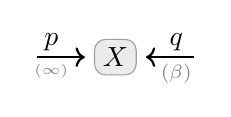
\begin{tikzpicture}[center base]
        \node[dpad0] (X) {$X$};
        \draw[arr, <-] (X) --
            node[above,inner sep=2pt, pos=0.65] {$p$}
            node[below,inner sep=2pt, pos=0.65]
                {${\color{gray}\scriptscriptstyle(\infty)}$}
             ++(-1.1,0);
        \draw[arr, <-] (X) --
            node[above,pos=0.6,inner sep=2pt]
            % {$\overset{\smash{\color{gray}(\beta)}}q$} ++(0.9, 0);
         	% {$\overset{{\color{gray}(\beta)}}q$}
            % {$q~^{{\color{gray}(\beta)}}$} ++(1.1, 0);
			{$q$}
			node[below,pos=0.6,inner sep=2pt]
                {$\scriptstyle{\color{gray}(\beta)}$}++(1.1, 0);
    \end{tikzpicture}}
	= \beta\, \kldiv pq .
\]
\end{prop}
\vskip-1.3ex
This result gives us an intuitive interpretation of the asymmetry of relative entropy / KL divergence, and a prescription about when it makes sense to use it.
$\kldiv p q$ is the inconsistency of a mental state containing both $p$ and $q$, when absolutely certain of $p$ (and not willing to budge on it).
This concords with the standard intuition that $\kldiv pq$ reflects the amount of information required to change $q$ into $p$, which is why
% some pronounce it in reverse, calling it
it is usually called the relative entropy ``from $q$ to $p$''.


% In general, we derive the following form for the inconsistency of a PDG whose contents are distributions $p(X)$ and $q(X)$, for arbitrary confidences.
We now consider the general case of a PDG comprising $p(X)$ and $q(X)$ with arbitrary confidences.
%, which we denote $\thickD^{PDG}_{r,s}(p,q)$,  .
\begin{linked}{lemma}{pdgdiv}
	% The PDG divergence $\thickD^{\mathrm{PDG}}_{(r,s)}(p, q)$,
    % The inconsistency of a PDG containing $p(X)$ with confidence $r$ and $q(X)$ with confidence $s$
    The inconsistency
	$\thickD^{\mathrm{P\mskip-2muD\mskip-1.5muG}}_{{\color{gray}(r,s)}}(p\Vert q)$
	of a PDG comprising $p(X)$ with confidence $r$ and $q(X)$ with confidence $s$
    is given in closed form by
	\vspace{-1ex}
    \[
		% \thickD^{\mathrm{PDG}}_{(r,s)}(p, q) :=
        \aar[\bigg]{\!\!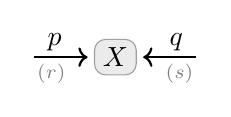
\begin{tikzpicture}[baseline = -0.75ex]
            \node[dpad0] (X) {$X$};
            \draw[arr2, <-] (X) --
			 		% node[above] {$\overset{(\beta : r)}p$}
			 		node[above, pos=0.6, inner sep=2pt, align=center] {$p$}
			 		node[below, pos=0.65, inner sep=2pt, align=center]
                        % {$\scriptstyle{\color{gray}(\beta : r)}$}
                        {$\scriptstyle{\color{gray}(r)}$}
				++(-1.1,0);
            \draw[arr2, <-] (X) --
					% node[above,pos=0.5] {$\overset{(\beta : s)}q$}
			 		node[above, pos=0.6, inner sep=2pt, align=center] {$q$}
			 		node[below, pos=0.65, inner sep=2pt, align=center]
                        % {$\scriptstyle{\color{gray}(\beta : s)}$}
                        {$\scriptstyle{\color{gray}(s)}$}
				 ++(1.1, 0);
        \end{tikzpicture}\!\!}
        % = \thickD^{\mathrm{PDG}}_{(r,s)}(p, q)
        = - (r+s) \log  \sum_x \left(p(x)^{r}\vphantom{\Big|} q(x)^{s}\right)^{\frac{1}{r+s}}.
        % = - (r+s) \log \sum_x \! \sqrt[\leftroot{0}\uproot{2}r+s]{\vphantom{\big|}p(x)^{r} q(x)^{s}}
    % \qquad\text{where}\qquad \xi:= \beta_p+\beta_q
    \]
\end{linked}
\vskip-1ex





Of the many generalizations of KL divergence, R\'enyi divergences, first characterized by Alfr\'ed R\'enyi \citeyear{renyi1961measures} are perhaps the most significant, as few others have found either application or an interpretation in terms of coding theory \parencite{van2014renyi}.
The R\'enyi divergence of order $\alpha$ between two distributions $p(X)$ and $q(X)$ is given by
\vspace{-1ex}
\begin{equation}
	\thickD_\alpha\infdivx p q := \frac{1}{1- \alpha} \log \sum_{x \in \V(X)} p(x)^\alpha q(x)^{1-\alpha}.  \label{eq:renyi}
\end{equation}
R\'enyi introduced this measure in the same paper as the more general
class of $f$-divergences, but directs his attention towards those of
%joe1
%the form \eqref{eq:renyi}, because satisfy a natural weakening of
%Fadeev's postulates \cite{fadeev1957begriff}, for Shannon entropy.
the form \eqref{eq:renyi}, because they satisfy a natural weakening of
standard postulates for Shannon entropy due to
% Fadeev \citeyear{fadeev1957begriff}.
\textcite{fadeev1957begriff}.
Concretely, every symmetric, continuous measure that additively separates over independent events, and with a certain ``mean-value property'', up to scaling,
% is a R\'enyi divergence \eqref{eq:renyi} for some $\alpha$, up to scaling \cite{renyi1961measures}.
is of the form \eqref{eq:renyi} for some $\alpha$ \parencite{renyi1961measures}.
It follows from \cref{lemma:pdgdiv} that
% varying the confidences of our two-distribution PDG carves out almost the same class:
% the inconsistency of our two-distribution PDG carves out almost the same class as we vary the confidences:
% carves out almost the same class:
% every R\'enyi divergence is the inconsistency of some PDG of this form, and
every R\'enyi divergence is a PDG divergence, and
every (non-limiting) PDG divergence is a (scaled) R\'enyi divergence.

%joe1: you[r talk about Renyi entropy and Renyi divergence.  Do you
%mean entropy?
%oli1: The divergence is more general; I'll just refer to that for consistency.
\begin{coro}[R\'enyi Divergences]
	% xx
    % \vskip-1em
	~\vspace{-1ex}
    \begin{align*}%
        % \thickD^{\mathrm{PDG}}_{r, s}(p, q)
        \aar[\Big]{\!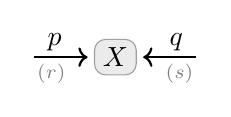
\begin{tikzpicture}[baseline = -0.75ex]
            \node[dpad0] (X) {$X$};
            \draw[arr2, <-] (X) --
			 		% node[above] {$\overset{(\beta : r)}p$}
			 		node[above, pos=0.6, inner sep=2pt, align=center] {$p$}
			 		node[below, pos=0.65, inner sep=2pt, align=center]
                        % {$\scriptstyle{\color{gray}(\beta : r)}$}
                        {$\scriptstyle{\color{gray}(r)}$}
				++(-1.1,0);
            \draw[arr2, <-] (X) --
					% node[above,pos=0.5] {$\overset{(\beta : s)}q$}
			 		node[above, pos=0.6, inner sep=2pt, align=center] {$q$}
			 		node[below, pos=0.65, inner sep=2pt, align=center]
                        % {$\scriptstyle{\color{gray}(\beta : s)}$}
                        {$\scriptstyle{\color{gray}(s)}$}
				 ++(1.1, 0);
        \end{tikzpicture}\!}
            &=
            s \cdot \thickD_{\frac{r}{r+s}}\infdivx{p}{q}
        % \qquad \text{and} \qquad
        \\[-1ex]\text{and}\qquad
        \thickD_{\alpha}\infdivx{p}{q}
        &=
        % \thickD^{\mathrm{PDG}}_{\left(\frac{\alpha}{1-\alpha}, 1\right)}(p, q).
        \aar[\Big]{\!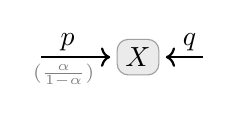
\begin{tikzpicture}[baseline = -0.75ex]
            \node[dpad0] (X) {$X$};
            \draw[arr2, <-] (X) --
			 		% node[above] {$\overset{(\beta : r)}p$}
			 		node[above, pos=0.6, inner sep=2pt, align=center] {$p$}
			 		node[below, pos=0.65, inner sep=2pt, align=center]
                        % {$\scriptstyle{\color{gray}(\beta : r)}$}
                        {$\scriptstyle{\color{gray}(\frac{\alpha}{1-\alpha})}$}
				++(-1.3,0);
            \draw[arr2, <-] (X) --
					% node[above,pos=0.5] {$\overset{(\beta : s)}q$}
			 		node[above, pos=0.6, inner sep=2pt, align=center] {$q$}
			 		% node[below, pos=0.65, inner sep=2pt, align=center]
                        % {$\scriptstyle{\color{gray}(\beta : s)}$}
                        % {$\scriptstyle{\color{gray}(s)}$}
				 ++(0.9, 0);
        \end{tikzpicture}\!}
    \end{align*}
\end{coro}
\vskip-1.4ex

However, the two classes are not identical, because the PDG divergences have extra limit points.
One big difference is that the reverse KL divergence $\kldiv q p$ is not a R\'enyi divergence $\thickD_\alpha\infdivx p q$ for any value (or limit) of $\alpha$.
% One big difference is that the reverse KL divergence $\kldiv q p$ is not a R\'enyi divergence $\thickD_\alpha\infdivx p q$ for any value (or limit) of $\alpha$.
This lack of symmetry has led others \parencite[e.g.,][]{cichocki2010families}
% to instead work with a re-scaled symmetric version of the R\'enyi entropy, called $\alpha$-divergence, which as an additional factor of $\frac1\alpha$.
to work instead with a symmetric variant called $\alpha$-divergence, rescaled by an additional factor of $\frac1\alpha$.
% \eqref{eq:alphadiv}  (although sometimes the term is used for the same quantity without the logarithm).
The relationships between these quantities can be seen in \cref{fig:statdistmap}.

% \begin{equation}
% 	\tilde \thickD_\alpha\infdivx p q := \frac{1}{\alpha( 1- \alpha)} \;{\color{black}\log}\!\! \sum_{x \in \V(X)} p(x)^\alpha q(x)^{1-\alpha} \label{eq:alphadiv}
% \end{equation}
%
%% What is the point of this paragraph? CUT.
% We submit that viewing these as inconsistencies can clarify things a great deal. Whereas the formula for R\'enyi entropy is mostly symmetric, the leading $\frac1{1-\alpha}$ of \eqref{eq:renyi} makes it instead \emph{skew}-symmetric, and as a result the behavior for $\alpha \in (0, \nicefrac12)$ is qualitatively different from the behavior for $\alpha \in (\nicefrac12, 1)$.
% PDG inconsistency, on the other hand, is symmetric: the semantics do not give special treatment to one edge over the other.


The Chernoff divergence measures the tightest possible exponential
bound on probability of error \parencite{nielsen2011chernoff} in Bayesian
%joe1
%hypotehsis testing.
hypothesis testing.
It also happens to be the smallest possible inconsistency of simultaneously believing $p$ and $q$, with total confidence 1.
\begin{coro}%[Chernoff Divergence as Inconsistency]
The Chernoff Divergence between $p$ and $q$ equals
\\[-1.8em]
% \vspace{-0.8em}
% \hfill
% \(
\[
	\inf_{\beta \in (0,1)}
	\aar[\Big]{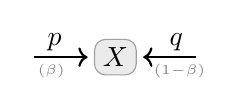
\begin{tikzpicture}[center base]
		\node[dpad0] (X) {$X$};
		\draw[arr2, <-] (X) --
			% node[above] {$\overset{(\beta)}p$}
			node[above, inner sep=2pt,pos=0.6] {$p$}
			node[below, inner sep=2pt,pos=0.65] {${\color{gray}\scriptscriptstyle(\beta)}$}
			 ++(-1.1,0);
		\draw[arr2, <-] (X) --
			% node[above,pos=0.5] {$\overset{(1-\beta)}q$}
			node[above, inner sep=2pt,pos=0.6] {$q$}
			node[below, inner sep=2pt, pos=0.65] {${\color{gray}\scriptscriptstyle(1-\beta)}$}
			++(1.1, 0);
	\end{tikzpicture}}.
	% = \thickD^{\mathrm{PDG}}_{(r,s)}(p, q)
	% = \thickD^{\text{Chernoff}}(p,q)
	% = - (r+s) \log \sum_x \! \sqrt[\leftroot{0}\uproot{2}r+s]{\vphantom{\big|}p(x)^{r} q(x)^{s}}
% \qquad\text{where}\qquad \xi:= \beta_p+\beta_q
\]
% \)
\end{coro}

One significant consequence of representing divergences as inconsistencies is that we can use \cref{lemma!} to derive relationships between them. The following facts follow directly from \cref{fig:statdistmap}, by inspection.
\begin{coro}
	\begin{enumerate}[nosep]
		\item R\'enyi entropy is monotonic in its parameter $\alpha$.
		% \item $\kldiv P Q \ge 2 \thickD_B(P,Q) \le \kldiv Q P$
		\item $\kldiv p q \ge 2 \thickD_B(p,q) \le \kldiv q p$.
		\item If $q(p > 0) < 1$ (i.e., $q \not\ll p$), then $\kldiv q p = \infty$.
	\end{enumerate}
\end{coro}


% Recall that these results are only for simple PDGs, which contain one variable and two distributions. Inconsistency of general PDGs, is in some sense a vast generalization of the Renyi divergences to arbitrary structured objects.
%
% Recall that all of these divergences correspond to PDGs containing only two distributions over one variable.
% Further properties can be proved with \cref{lemma!}:
% All of these divergences correspond to PDGs of only two distributions and one variable.
These divergences correspond to PDGs with only two edges and one variable.
%
What about more complex graphs?
% For a start, it is not difficult to see that the usual notion of conditional divergences
% For a start, the usual notion of conditional divergences
For a start, the usual notion of a conditional divergence
% $\thickD_{\bullet}\big(p(\!Y\!|\!X\!) \,\Vert\, q(\!Y\!|\!X\!) \,|\, r(\!X\!)\big)$
\def\ns{\mskip-1.5mu}
$
\thickD^{\mathrm{P\mskip-2muD\mskip-1.5muG}}_{r,s}\ns(p(\ns Y \ns|\ns X \ns) \,\Vert\, q(\ns Y \ns|\ns X\ns) \,|\, r(\ns X\ns)\ns)
\!:=\!
 \displaystyle \Ex_{x\sim r} \! \thickD^{\mathrm{P\mskip-2muD\mskip-1.5muG}}_{r,s}\ns(p(\ns Y \ns|x) \,\Vert\, q(\ns Y \ns|x)\!\big)
$
% straightforwardly falls out of PDGs of the form
% falls out of PDGs of the form
can be represented straightforwardly as
\vskip-3ex
% \!
\[
% \begin{tikzpicture}[center base]
% 	\node[dpad0] (X) at (0,0) {$X$};
% 	\node[dpad0] (Y) at (1.25,0) {$Y$};
% 	\draw[arr1, <-] (X) --
% 		node[above, pos=0.55, inner sep=2pt]{$r$}
% 		node[below, pos=0.55, inner sep=2pt]{${\color{gray}\scriptscriptstyle(\infty)}$}
% 		+(-1,0);
% 	\draw[arr1] (X) to[bend left=25, inner sep=1pt]
% 		node[fill=white, inner sep=1pt, pos=0.35] {$p$}
% 		node[above, inner sep=2pt, pos=0.68]
% 			{${\color{gray}\scriptscriptstyle(r)}$}
% 		(Y);
% 	\draw[arr1] (X)
% 		to[bend right=25]
% 		node[fill=white, inner sep=1pt,pos=0.35] {$q$}
% 		node[below, inner sep=2pt, pos=0.68]
% 			{${\color{gray}\scriptscriptstyle(s)}$}
% 		(Y);
% \end{tikzpicture}\,.
\thickD^{\mathrm{P\mskip-2muD\mskip-1.5muG}}_{r,s}\ns(p \,\Vert\, q \,|\, r\ns)
 = \aar*{
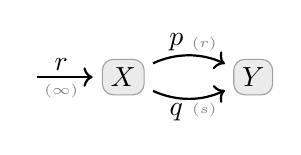
\begin{tikzpicture}[center base]
	\node[dpad0] (X) at (0,0) {$X$};
	\node[dpad0] (Y) at (1.65,0) {$Y$};
	\draw[arr, <-] (X) --
		node[above, pos=0.55, inner sep=2pt]{$r$}
		node[below, pos=0.55, inner sep=2pt]{${\color{gray}\scriptscriptstyle(\infty)}$}
		+(-1.2,0);
	\draw[arr] (X) to[bend left=25, inner sep=1pt]
		% node[fill=white, inner sep=2pt, pos=0.35] {$p$}
		node[above, inner sep=2pt, pos=0.35] {$p$}
		node[above, inner sep=2pt, pos=0.68]
			{${\color{gray}\scriptscriptstyle(r)}$}
		(Y);
	\draw[arr] (X)
		to[bend right=25]
		% node[fill=white, inner sep=2pt,pos=0.35] {$q$}
		node[below, inner sep=2pt,pos=0.35] {$q$}
		node[below, inner sep=2pt, pos=0.68]
			{${\color{gray}\scriptscriptstyle(s)}$}
		(Y);
\end{tikzpicture}
}
\,.
\]
\vskip-2ex
% and in general,
% The inconsistency of a PDG can be viewed as a vast generalization of these divergences to arbitrary structured objects.
% \Cref{lemma!}, together with minor structural manipulation, gives visual proofs of standard divergence properties.
% Such graphs are also useful intermediates.
Other structures are useful intermediates.
% \Cref{lemma!} in conjunction with structural manipulation, yields visual proofs of many properties of these divergences.
%oli3: better wording.
% \Cref{lemma!}, plus some structural manipulation, yields visual proofs of many divergence properties; a proof of the data-processing inequality can be seen in \Cref{fig:dpi-vis-proof}.
\Cref{lemma!}, plus some structural manipulation, gives visual proofs of many divergence properties; \Cref{fig:dpi-vis-proof} features such a proof of the data-processing inequality.
And in general, PDG inconsistency can be viewed as a vast generalization of divergences to arbitrary structured objects.

\begin{figure*}
	\tikzset{ci2/.style={inner sep=2pt, align=center}}%
	%
	\colorlet{pcolor}{Plum}%
	\colorlet{qcolor}{MidnightBlue}%
	\def\amt{45}%
	\tikzset{pstyle/.style={line width=0.9pt, pcolor!\amt!black}}%
	\tikzset{qstyle/.style={line width=1.3pt, qcolor!\amt!black}}%
	\tikzset{pqstyle/.style={line width=1.5pt,pcolor!50!qcolor!\amt!black}}%
	%
	\def\lgs{\color{gray!80}\scriptstyle}%
	\def\plabel{{$\lgs\color{pcolor!40}({\beta})$}}
	\def\qlabel{{$\lgs\color{qcolor!40}({\zeta})$}}
	%
	% {\color{structurecolor}
		% \[ \pdgdiv pq \ge \pdgdiv {f\circ p}{f \circ q}\]}%
	%
	\scalebox{0.89}{{
	% \begin{equation*}%
	% \[
	$
	% - \log \Pr\nolimits_{p,d}(X\!=\!x) ~=\qquad&\\
	\aar*{\!\begin{tikzpicture}[center base]
	   \node[dpad0] (X) {$X$};
	   \draw[arr2, <-,qstyle] (X) --
		  node[above,pos=0.6,ci2]{$q$}
				 % node[above,pos=0.6]{$q^{{\color{gray}(s)}}$}
				node[below, pos=0.65,ci2] {\qlabel}
		   ++(1.1, 0);
	   \draw[arr2, <-,pstyle] (X) --
				node[above,pos=0.6,ci2]{$p$}
		   % node[above,pos=0.6]{$p^{{\color{gray}(r)}}$}
				node[below, pos=0.65, ci2] {\plabel}
		   ++(-1.1, 0);%
	\end{tikzpicture}\!}
	\!=\!\!
	\aar**{\!\begin{tikzpicture}[center base]
	   \node[dpad0] (X) {$X$};
	   \node[dpad0,above=.8 of X,align=center] (Y) {$Y$};
	   \draw[arr2, <-,qstyle] (X) --
			node[above,pos=0.7,ci2]{$q$}
						node[below, pos=0.65,ci2] {\qlabel}
		   ++(1.1, 0);
	   \draw[arr2, <-,pstyle] (X) --
		  node[above,pos=0.7,ci2]{$p$}
						node[below, pos=0.65,ci2] {\plabel}
		   ++(-1.1, 0);%
	   \draw[arr2, pqstyle] (X) --
		  node[left,pos=0.45,inner sep=1pt]{$f$}
						node[right, pos=0.45, inner sep=1.5pt, align=center] % below,rotate=90
							{{$\lgs\color{pcolor!50!qcolor!40}(\beta+\zeta)$}}
		  (Y);%
	\end{tikzpicture}\!}
	\!=\!
	\aar**{\!\begin{tikzpicture}[center base]
	   \node[dpad0] (X1) {$X_1$};
	   \node[dpad0, right=0.6 of X1] (X2) {$X_2$};
	   \node[dpad0,above=.8 of {$(X1)!.5!(X2)$},align=center] (Y) {$Y$};
	   \draw[arr2, -, double equal sign distance] (X1) to (X2);
	   \draw[arr2, <-,qstyle] (X2) --
		  node[above,pos=0.6,ci2]{$q$}
						node[below, pos=0.65,ci2] {\qlabel}
		  ++(1.1, 0);
	   \draw[arr2, <-,pstyle] (X1) --
		  node[above,pos=0.6,ci2]{$p$}
						node[below, pos=0.65,ci2] {\plabel}
		  ++(-1.1, 0);%
	   \draw[arr2,pstyle] (X1) to[bend left=40]
		  node[above left, pos=0.35, inner sep=1pt]{$f$}
						node[below right=0 and 0, pos=0.45, inner sep=0pt, align=center] {\plabel}
		   (Y);%
	   \draw[arr2,qstyle] (X2) to[bend right=40]
		  node[above right, pos=0.35, inner sep=1pt]{$f$}
						node[below left=0 and 0, pos=0.45, inner sep=0pt, align=center] {\qlabel}
		   (Y);%
	\end{tikzpicture}\!}
	\!\ge\!
	\aar**{\!\begin{tikzpicture}[center base]
		   \node[dpad0] (X1) {$X_1$};
		   \node[dpad0, right=0.65 of X1] (X2) {$X_2$};
		   \node[dpad0,above=.75 of {$(X1)!.5!(X2)$},align=center] (Y) {$Y$};
		   \draw[arr2, <-,qstyle] (X2) --
			  node[above,pos=0.6,ci2]{$q$}
							node[below, pos=0.65,ci2] {\qlabel}
			  ++(1.1, 0);
		   \draw[arr2, <-,pstyle] (X1) --
			  node[above,pos=0.6,pstyle,ci2]{$p$}
							node[below, pos=0.65,ci2] {\plabel}
			  ++(-1.1, 0);%
		   \draw[arr2,pstyle] (X1) to[bend left=30]
			  node[above left, pos=0.35, inner sep=1pt]{$f$}
							node[below right=0 and 0, pos=0.45, inner sep=0pt, align=center] {\plabel}
			   (Y);%
		   \draw[arr2,qstyle] (X2) to[bend right=30]
			  node[above right, pos=0.35, inner sep=1pt]{$f$}
							node[below left=0 and 0, pos=0.45, inner sep=0pt, align=center] {\qlabel}
			   (Y);%
		\end{tikzpicture}\!}
	\!\!=\!
	\aar*{\!\begin{tikzpicture}[center base]
	   \node[dpad0] (X) {$X$};
	   \draw[arr2, <-,qstyle] (X) --
		   node[above,pos=0.7,ci2]{$ f\!\circ\! q$}
				 node[below, pos=0.65,ci2] {\qlabel}
		   ++(1.1, 0);
	   \draw[arr2, <-,pstyle] (X) --
		   node[above,pos=0.6,ci2]{$ f\!\circ\! p$}
				 node[below, pos=0.65,ci2] {\plabel}
		   ++(-1.1, 0);%
	\end{tikzpicture}\!}
	% \end{equation*}
	% \]
	$
	}}
	\def\pdgdiv{\thickD^{\mathrm{P\mskip-2muD\mskip-1.5muG}}_{\lgs({\color{pcolor!40}\beta},{\color{qcolor!40}\zeta})}\infdivx[\big]}
	\caption{A visual proof of the data-processing inequality:
	 	$\pdgdiv pq \ge \pdgdiv {f\circ p}{f \circ q}$.
	In words:
	% A verbal summary:
	the cpd $f(Y|X)$ can always be satisfied, so adds no inconsistency.
	It is then equivalent to split $f$ and the variable $X$ into $X_1$ and $X_2$ with edges enforcing $X_1 = X_2$.
	% Then, split $f$ and the variable $X$ into $X_1$ and $X_2$ with edges enforcing $X_1 = X_2$.
	But removing such edges can only decrease inconsistency. 
	Finally, compose the remaining cpds to give the result. 
	% A full justification can be found in the appendix.
	See the appendix for a full justification.
	}
	\label{fig:dpi-vis-proof}
\end{figure*}

\section{VARIATIONAL OBJECTIVES AND BOUNDS}
\label{sec:theory}

% The fact that the incompatibility of $\dg M$ with a \emph{specific} joint distribution $\mu$ is an upper bound on the inconsistency (i.e., the score of the \emph{best} such joint distribution) is not a deep one (although it does suggest a variational approach to inference in PDGs, which we describe in parallel work).
% % but it does yield an efficient approximate inference procedure for PDGs: choose a tractable parametric family $\mathcal P$ of joint distributions $\mu$, and optimize \eqref{eq:semantics}. Making this precise is the focus of a parallel work.
% Here, we focus on the more surprising converse:  PDG semantics capture interesting features of variational inference and provides a graphical proof language for it.
% %, which can be notoriously difficult to track symbolically.
%
% Using PDGs to describe variational models not only reproduces the standard objectives, but also provides a graphical language for variational inference.

The fact that the incompatibility of $\dg M$ with a \emph{specific} joint distribution $\mu$ is an upper bound on the inconsistency is not a deep one, but it is of a variational flavor.
% % but it does yield an efficient approximate inference procedure for PDGs: choose a tractable parametric family $\mathcal P$ of joint distributions $\mu$, and optimize \eqref{eq:semantics}. Making this precise is the focus of a parallel work.
Here, we focus on the more surprising converse:  PDG semantics capture general aspects of variational inference and provide
a graphical proof language for it.
% a graphical language for reasoning about it.

\subsection{PDGs and Variational Approximations}
\label{sec:variational}

We begin by recounting the standard development of the `Evidence Lower BOund' (ELBO), a standard objective for training latent variable models \parencite[\S2.2]{blei2017variational}.
%oli2: not necessary
% and then show that it arises naturally as the inconsistency of the obvious PDG.
%
Suppose we have a model $p(X,Z)$, but only have access to observations of $x$.
In service of adjusting $p(X,Z)$ to make our observations more likely, we would like to maximize $\log p(X\!\!=\!x)$, the ``evidence'' of $x$ (\Cref{prop:marginal-ll}).
% Unfortunately, computing $p(X) = \int p(X,z)\, \mathrm d z$ requires integrating over $Z$, which can be intractable.
Unfortunately, computing $p(X) = \sum_z p(X,Z\!\!=\!z)$ requires summing over all of $Z$, which can be intractable.
%
% The variational approach is as follows: fix a family of distributions $\mathcal Q$ that is easy to sample from, choose some $q \in \mathcal Q$, and assume that $Z \sim q$.
% ; to start, we guess $q_0(Z)$.
% Now it's easy to sample $Z$ (by assumption), but $q_0$ is likely to be inconsistent with $p$. But if, while optimizing $p$ to best fit the data, we also optimize $q$ so that it closly mirrors $p$, (and if $\mathcal Q$ is expressive enough), we can avoid computing the ``evidence''  $\log p(x) = \log \int p(x,z)\, \mathrm d z$.
%% For fixed $p$, we are interested in $q^*_p := \argmin_{q \in \mathcal Q} \kldiv{q(Z)}{p(Z\mid x)}$.
% But only by being clever. The straightforward divergence-minimizing approach to both optimization problems (the choice of $p$ and $q$) requires computing this integral \cite[\S2.2]{blei2017variational}. Instead, $q$ and $p$ are chosen so as to maximize
% Now, we can sample $Z$ from $q$, so we can compute
% $
%     \Ex_{z \sim q} \frac{p(x,z)}{q(z)} =
%     \int_{z} q(z) \frac{p(x,z)}{q(z)} \mathrm dz=
%     \int p(x,z) \mathrm d z = p(z)
% $
The variational approach is as follows: fix a family of distributions $\mathcal Q$ that is easy to sample from, choose some $q(Z) \in \mathcal Q$, and define
$\mathrm{ELBO}_{p,q}(x) := \Ex_{z \sim q} \log \frac{p(x,z)}{q(z)}$.
This is something we can estimate, since we can sample from $q$. By Jensen's inequality,
\[
    \mathop{\mathrm{ELBO}}\limits_{p,q}(x)
    =\! \Ex_{q} \log \frac{p(x,Z)}{q(Z)}
    % = \int_{z} q(z) \log  \frac{p(x,z)}{q(z)} \mathrm dz
    \le  \log \Big[\! \Ex_{q}\! \frac{p(x,Z)}{q(Z)} \Big]\!
    % = \log p(X),
	%oli3:
    = \log p(x),
    % \int p(x,z) \mathrm d z = p(z)
\]
with equality if $q(Z) = p(Z)$.
%oli3:
% So to maximize $p(X)$, it suffices to adjust $p$ and $q$ to maximize $\mathrm{ELBO}_{p,q}(x)$,%
So to find $p$ maximizing $p(x)$, it suffices to adjust $p$ and $q$ to maximize $\mathrm{ELBO}_{p,q}(x)$,%
    \footnote{For many iid samples: $\max_{p,q}\sum_{x \in \xsamp}\mathrm{ELBO}_{p,q}(x)$.}
 provided $\mathcal Q$ is expressive enough.

% $\mathrm{ELBO}_{p,\xsamp}(q) :=
%     \sum_{x \in \xsamp} \mathrm{ELBO}_{p,q}(x)
% $.
% where
% \begin{equation}
% 	% \mathrm{ELBO}_{p,\xsamp}(q) :=
% 	%  	\sum_{x \in \xsamp} \mathrm{ELBO}_{p,q}(x)~,
% 	% \qquad \qquad\text{where}
%     %\qquad
% 	\mathrm{ELBO}_{p,q}(x) := \Ex_{z \sim q} \log \frac{p(x,z)}{q(z)}, \label{eq:elbo}
% \end{equation}

% We will now see that this tie extends to latent variable models in a nice way.
The formula for the ELBO is somewhat difficult to make sense of.%
\footnote{Especially if $p$ and $q$ are densities. See \cref{appendix:density}}
% (see \cref{remark:continuous}).
% in which case the units don't cancel in the logarithm, making it an ill-defined physical quantity (see \cref{remark:continuous}).
%joe1*: mass functions comes completely out of the blue here.  If you
%mean mass functions as in Demspter-Shafer, then you must explain
%this.  Actually, whatever you mean, you must explain it.  Idon't see
%where this interpretation has any impact on your propositin.
% DONE
% Nevertheless, if we interpret $p$ and $q$ are mass functions, it turns
% out that the ELBO also arises naturally as the inconsistency of the
Nevertheless, it arises naturally as the inconsistency of the
appropriate PDG.

\begin{linked}{prop}{pdg-elbo-x}%[Capturing the ELBO]
		% \label{prop:pdg-elbo-x}
	% If $p(X,Z)$ is a joint probabilistic model of observed variables $X$ and hidden variables $Z$, and $q(Z)$ is any distribution
	% That is,
	The negative ELBO of $x$ is the inconsistency of the PDG containing $p$,$q$, and $X\!\!=\!x$, with high confidence in $q$.
	That is,
    \vspace{-0.8em}
	\[
	-\mathrm{ELBO}_{p,q}(x) =
		% \lim_{t \to \infty}
	 \aar[\Bigg]{
% 	  \Inc\left(
		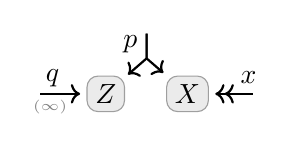
\begin{tikzpicture}[center base]
			\node[dpad0] (Z) {$Z$};
			\node[dpad0,right=.5 of Z] (X) {$X$};
			\coordinate (A) at ($ (X)!.5!(Z) + (0,0.8)$);
			\draw[arr1] (A) -- node[left, inner sep=3pt]{$p$} ++(0,-0.35) -- (X);
			\draw[arr1] (A) -- ++(0,-0.35) -- (Z);
%
			\draw[arr2, <<-] (X) --  node[above,pos=0.8]{$ x$} ++(0.9, 0);
			\draw[arr2, <-] (Z) --
                node[above,pos=0.65, inner sep=2pt]{$q$}
                node[below,pos=0.7, inner sep=2pt]{${\color{gray}\scriptscriptstyle(\infty)}$}
                ++(-0.9, 0);%
			%\scriptstyle q^{\{\beta =\infty\}}
			% \ar[r,"p"] \& Z \ar[r,"p", bend left] \& X \ar[l,"q", bend left] \& \ar[l, two heads, "x"']
		\end{tikzpicture}
		}%_{\!\!0}
% 		\right)
		.
	\]
\end{linked}
\vskip-1ex



%
% The proof of \cref{prop:pdg-elbo-x} %, lke that of \cref{prop:pdg-Ix},
%  hinges critically on the fact that we force a single sample $x$; its PDG does not capture the whole context $\xsamp$.
% Nevertheless, we get an analogous result when we replace the sample $x$ with the entire data distribution $\datadist\xsamp$, which differs only in that the expression is offset by the entropy of the data distribution.
%
%
%
% \begin{proof}
%
% \end{proof}



% The use of the ELBO as an objective is often justified by the fact that it is a lower bound on the log likelihood of partial observation $X=x$ (the evidence), which is usually proved with some algebra and Jensen's inequality.
% , or alternatively, but appeal to the non-negativity of relative entropy \cite{elboproofs}.
Owing to its structure, a PDG is often more intuitive and easier to work with than the formula for its inconsistency.
To illustrate,
we now give a simple and visually intuitive proof of the bound traditionally used to motivate the ELBO, via \cref{lemma!}:
% We now give a very simple diagrammatic proof by via \cref{lemma!}:
% $\log \frac1{p(x)} = $
% \vskip-2ex
\[
\log \! \frac{1}{p(\mskip-1.5mux\mskip-1.5mu)} \!=\!\!
	 \aar*{
		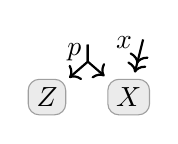
\begin{tikzpicture}[center base]
			\node[dpad0] (Z) {$Z$};
			\node[dpad0,right=.5 of Z] (X) {$X$};
			\coordinate (A) at ($ (X)!.5!(Z) + (0,0.7)$);
			\draw[arr1] (A) -- node[left, inner sep=2pt]{$p$} ++(0,-0.25) -- (X);
			\draw[arr1] (A) -- ++(0,-0.25) -- (Z);
			% \draw[arr2, <<-] (X) --  node[above,pos=0.8]{$ x$} ++(0.9, 0);
			\draw[arr2, <<-] (X) --  node[left,pos=0.8]{$x$} ++(0.2, 0.8);
		\end{tikzpicture}
		}%_{\!\!0}
	\!\le\!
    % \lim_{t \to \infty}
	 \aar*{\!\!
% 	  \Inc\left(
		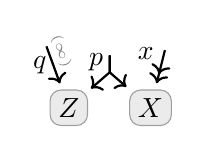
\begin{tikzpicture}[center base]
			\node[dpad0] (Z) {$Z$};
			\node[dpad0,right=.5 of Z] (X) {$X$};
			\coordinate (A) at ($ (X)!.5!(Z) + (0,0.7)$);
            \draw[arr1] (A) -- node[left, inner sep=2pt]{$p$} ++(0,-0.25) -- (X);
			\draw[arr1] (A) -- ++(0,-0.25) -- (Z);
%
			% \draw[arr2, <<-] (X) --  node[above,pos=0.8]{$ x$} ++(0.9, 0);
            \draw[arr2, <<-] (X) --  node[left,pos=0.8]{$x$} ++(0.2, 0.8);
			% \draw[arr2, <-] (Z) -- node[above,pos=0.6]{$ q!$} ++(-0.9, 0);%
			\draw[arr2, <-] (Z) -- node[left, inner sep=2pt,pos=0.5]{$q$}
                node[above, inner sep=1.5pt, rotate=-70, pos=0.7]{{${\color{gray}\scriptscriptstyle(\infty)}$}}
                % ++(-0.9, 0.0);
                ++(110:0.9);
                % ++(-0.3, 0.75);%
			% \ar[r,"p"] \& Z \ar[r,"p", bend left] \& X \ar[l,"q", bend left] \& \ar[l, two heads, "x"']
		\end{tikzpicture}
		}%_{\!\!0}
% 		\right)
    \!=\! -\!\mathop{\mathrm{E\mskip-0.5muL\mskip-0.5muB\mskip-0.5muO}}\limits_{p,q}(\mskip-1.5mux\mskip-1.5mu).
\]
% $= - \mathrm{ELBO}_{p,q}(x)$.
% \footnotemark[\thefootnote]~
The first and last equalities are \Cref{prop:marginal-ll,prop:pdg-elbo-x} respectively.
 % and the inequality is an instance of \Cref{lemma!}.
%% This is fine material, but we don't have space for it...
% We submit that this proof is more intuitve and gives a clearer picture of why it should be true. The second PDG has more edges, so it must be at least as inconsistent.
% Furthermore, this picture shows us that if we simultaneously vary $q(Z)$ within an expressive enough class of distributions, the inequality is also tight, because the distribution that realizes the smallest inconsistency must have some marginal on $Z$ --- and taking $q$ to be that distribution will incur no additional inconsistency.
%oli2:
% We submit that our presentation has substantial pedagogical benefits.
Now to reap some pedagogical benefits.
The second PDG has more edges so it is clearly at least as inconsistent. Furthermore, it's easy to see that equality holds when $q(Z) \!=\! p(Z)$: the best distribution for the left PDG has marginal $p(Z)$ anyway, so insisting on it incurs no further cost.
% so the constraint is already satisfied.

 % We also have analog analog holds for the entire dataset at once, which is more easily formulated with a slightly different variational form in the next section.

% \begin{align*}
% \ell(p;\xsamp) &=
% 	 \aar[\Bigg]{
% 	 % \Inc\left(
% 		\begin{tikzpicture}[center base]
% 			\node[dpad0] (Z) {$Z$};
% 			\node[dpad0,right=.5 of Z] (X) {$X$};
% 			\coordinate (A) at ($ (X)!.5!(Z) + (0,0.7)$);
% 			\draw[arr1] (A) -- node[right]{$ p$} ++(0,-0.25) -- (X);
% 			\draw[arr1] (A) -- ++(0,-0.25) -- (Z);
% %
% 			\draw[arr1, <<-] (X) --  node[above,pos=0.8]{$ \datadist\xsamp$} ++(0.9, 0);
% 			% \draw[arr1, <-] (Z) -- node[above]{$ q$} ++(-0.9, 0);
% 		\end{tikzpicture}
% 		}%_{\!\!0}
% 		% \right)
% 		 + \H(\datadist\xsamp) \\
% 		&\le
% 			\lim_{t \to \infty}
% 		  \aar[\Bigg]{
% 		  \begin{tikzpicture}[center base]
% 	  		\node[dpad0] (Z) {$Z$};
% 	  		\node[dpad0,right=.5 of Z] (X) {$X$};
% 	  		\coordinate (A) at ($ (X)!.5!(Z) + (0,0.7)$);
% 	  		\draw[arr1] (A) -- node[right]{$ p$} ++(0,-0.25) -- (X);
% 	  		\draw[arr1] (A) -- ++(0,-0.25) -- (Z);
% 	  %
% 	  		\draw[arr1, <-] (X) --  node[above,pos=0.2,anchor=south west]{$ {\datadist\xsamp}^{\{\beta= t\}}$} ++(0.9, 0);
% 	  			% ^{\{\beta=\beta_0\}}
% 	  		\draw[arr1, <-] (Z) -- node[above]{$q^{\{\beta= t\}} $} ++(-0.9, 0);
% 	  	\end{tikzpicture} } + \H(\datadist\xsamp) = - \Ex_{\datadist\xsamp} \mathrm{ELBO}_{p,q}(X),
% \end{align*}
% which holds for the same reason.


\subsection{Variational Auto-Encoders and PDGs}

An autoencoder is a probabilistic model intended to compress a
variable $X$ (e.g., an image) to a compact latent representation
$Z$.
% $Z$ (e.g., a vector).
Its structure is given by two conditional distributions:
an encoder $e(Z | X)$, and a decoder $d(X | Z)$.
Of course, not all pairs of cpds fill this role equally well.
% Perhaps most importantly, we would like to have low
One important consideration is the
% \emph{reconstruction error} \eqref{eq:rec}---when we decode an encoded $x$, we would like it to be reasonably similar to the original.
\emph{reconstruction error} \eqref{eq:rec}: when we decode an encoded image, we would like it to resemble the original.
\vspace{-0.5em}
\begin{equation}
	% \mathrm{Rec}(x) := \!\! \Ex_{z \sim e \mid x} \, \underbrace{\,\mathrm I_{d\mid z}(x)~\vphantom{\Big|}}_{\mathclap{\left(\;\substack{\text{additional bits required to}\\\text{decode $x$ from $z$, its encoding}}\;\right)}}
	% \!= \sum_z e(z \,|\, x) \log \frac1{d(x \,|\, z)}\label{eq:rec}
	%
	\mathrm{Rec}(x) := \!\!\!\!\! \Ex_{z \sim e(Z|x)} \smash{\underbrace{\mathrm I_{d(\!X\!|z)}(x)\vphantom{\Big|}}_{\mathclap{\left(\;\substack{\text{additional bits required to}\\\text{decode $x$ from its encoding  $z$}}\;\right)}}}
	\!= \sum_z e(z \,|\, x) \log \frac1{d(x \,|\, z)}\label{eq:rec}
\end{equation}
\vspace{0.0ex}
%
% It just so happens that $\mathrm{Rec}(x) =
% \aar*{\begin{tikzpicture}[center base]
%     \node[dpad0] (Z) {$Z$};
%     \node[dpad0,right=.6 of Z] (X) {$X$};
%     \draw[arr2, ->] (X) to[bend left=60]
%         node[below, inner sep=2pt]{$e$}
%         node[above, inner sep=2pt]{${\color{gray}\scriptscriptstyle(\infty)}$} (Z);
%     \draw[arr2, ->] (Z) to[bend left=50]
%         node[above, inner sep=2pt]{$d$} (X);
%     \draw[arr2, <<-] (X) --
%         node[above,pos=0.8]{$x$}
%         ++(0.9, 0);
% \end{tikzpicture}}$.
% Note the similarity to the cross entropy objective from before, except in place of our


%DONE reclaim space
% There are other desiderata as well. It would be nice if the distribution on $Z$ had a nice form---perhaps factoring into independent features, which we might use to describe $X$.
There are other desiderata as well. Perhaps good latent representations $Z$ have uncorrelated components, and are normally distributed.
%joe1*: I don't see how beliefs can encode wishes at all. Wishes are
%captured by utilities, not probabilities.  I'm lost.
%oli1: the whole point is that probabilities/objectives
% are a blurred line. I'll tweak the wording a little.
% this wish in the form of a belief $p(Z)$, known as a variational
% We encode this kind of wishful thinking as a belief $p(Z)$, known as a variational prior.
We encode such wishful thinking as a belief $p(Z)$, known as a variational prior.

The data of a \emph{variational} auto-encoder
\parencite{kingma2013autoencoding}
consists of $e(Z|X)$, $d(X|Z)$, and $p(Z)$.
The encoder $e(Z|X)$ can be used as a variational approximation of $Z$, differing from $q(Z)$ of \Cref{sec:variational} only in that it can depend on $X$. Here, the analog of the ELBO becomes
\vspace{-0.5ex}
\begin{align*}
	\mathrm{ELBO}_{p,e,d}(x) :=&
		% \Ex_{z \sim e|x}
		\Ex_{z \sim e(Z|x)} \left[\log \frac{p(z) d(x\mid z)}{e(z\mid x)} \right] \\
		% \Ex_{e(Z|x)} \left[\log \frac{p(Z) d(x\mid Z)}{e(Z\mid x)} \right] \\
		% &= \Ex_{z \sim e|x}\left[ \log \frac{p(z)}{e(z\mid x)}  \right] - \Ex_{z \sim e|x} \log \frac1{d(x\mid z)} \\
		=& - \mathrm{Rec}(x) - \kldiv{e(Z|x)}{p}.
\end{align*}
\vspace{-3ex}

This gives us the following analog of \cref{prop:pdg-elbo-x}.

\begin{linked}{prop}{pdg-elbo-vae}
	The VAE loss of a sample $x$
    % \dfootnote{\label{fn:multisample}See appendix for a multi-sample analog.}
    is the inconsistency of the PDG comprising the encoder
	$e$
	(with high confidence, as it defines the encoding),
	decoder
	$d$, prior $p$, and $x$.
	That is,
    % \vspace{-1.8em}
    \vspace{-3ex}
	\[
	-\mathrm{ELBO}_{p,e,d}(x) =
	 \aar*{
		% \begin{tikzcd}[AmpRep,row sep=1em,column sep=1.5em]
		% 	\ar[r,"p"] \& Z \ar[r,"d", bend left] \& X \ar[l,"e!", bend left] \& \ar[l, two heads, "x"']
		% \end{tikzcd}
		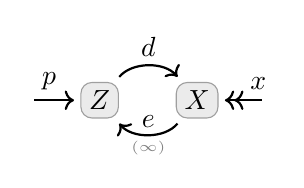
\begin{tikzpicture}[center base]
			\node[dpad0] (Z) {$Z$};
			\node[dpad0,right=.7 of Z] (X) {$X$};
			\draw[arr2, ->] (X) to[bend left=50]
				node[above, inner sep=2pt]{$e$}
				node[below, inner sep=2pt]{${\color{gray}\scriptscriptstyle(\infty)}$}
                (Z);
			\draw[arr2, ->] (Z) to[bend left=50]
				node[above]{$ d$} (X);
			\draw[arr2, <<-] (X) --
			  	node[above,pos=0.8]{$ x$}
			 	++(0.9, 0);
			\draw[arr2, <-] (Z) --
				node[above,pos=0.6]{$ p$}
				++(-0.9, 0);%
		\end{tikzpicture}}.
 	\]
    \vspace{-4ex}
\end{linked}


%DONE text needs cleaning up.
% \subsection{Intuitive Proofs of Variational Bounds}\label{sec:variational-bounds}
%
% \Cref{prop:pdg-elbo-vae,prop:pdg-elbo-vae-whole} can be used to derive another variational bound. Once again, the addition of the edge $e$ cannot decrease the inconsistency (\cref{lemma!}), but believing it with high confidence does make it possible to know the encoding of a sample, making inference tractable.
% We now use \Cref{prop:pdg-elbo-vae,prop:marginal-ll,lemma!} to derive another variational bound:
We now give a visual proof of the analogous variational bound.
% Let $\Pr_{p,d}(X,Z) := p(Z)d(X|Z)$ be
% Let $pd(X,Z) := p(Z)d(X|Z)$ be
Let $\Pr_{p,d}(X,Z) := p(Z)d(X|Z)$ be
% the joint distribution arising from decoding samples from the prior. Then,
the distribution that arises from decoding the prior. Then:
%joe1: the layout here needs to be improved
%DONE
% ~~$- \log \Pr(x) =$
% \vspace{-1.2em}
% \[
% 	\aar[\bigg]{\begin{tikzpicture}[baseline=-0.5ex]
% 	   \node[dpad0] (Z) {$Z$};
% 	   \node[dpad0,right=.6 of Z] (X) {$X$};
% 	   \draw[arr2, ->] (Z) to[bend left=30]
% 		   node[above]{$ d$} (X);
% 	   \draw[arr2, <<-] (X) --
% 		   node[above,pos=0.8]{$ x$}
% 		   ++(0.9, 0);
% 	   \draw[arr2, <-] (Z) --
% 		   node[above,pos=0.6]{$ p$}
% 		   ++(-0.9, 0);%
% 	\end{tikzpicture}}
%  	\le
%  	\aar*{
%    \begin{tikzpicture}[center base]
%        \node[dpad0] (Z) {$Z$};
%        \node[dpad0,right=.7 of Z] (X) {$X$};
%        \draw[arr2, ->] (X) to[bend left=50]
%            node[above, inner sep=2pt]{$e$}
%            node[below, inner sep=2pt]{${\color{gray}\scriptscriptstyle(\infty)}$}
%            (Z);
%        \draw[arr2, ->] (Z) to[bend left=30]
%            node[above]{$ d$} (X);
%        \draw[arr2, <<-] (X) --
%            node[above,pos=0.8]{$ x$}
%            ++(0.9, 0);
%        \draw[arr2, <-] (Z) --
%            node[above,pos=0.6]{$ p$}
%            ++(-0.9, 0);%
%    \end{tikzpicture}}
% \]
% \vskip-1.2em
% $= -\mathrm{ELBO}_{p,e,d}(x).$
% \vspace{-1.2em}
\begin{align*}
	\log \frac{1}{\displaystyle\!\mathop{\mathrm{P\mkern-1.5mur}}_{\mathclap{p\mkern-1mu,d}}(\mskip-1.5mux\mskip-1.5mu)\!} \!=\!
	% \log \frac{1}{\displaystyle pd(\mskip-1.5mux\mskip-1.5mu)\!} \!=\!
	% - \log {\Pr(x)} =
	% \qquad &\\
	% \aar[\Bigg]
	\aar**
	{$\mkern-1mu$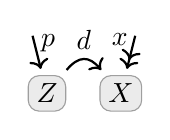
\begin{tikzpicture}
			% [baseline=2.1ex]
			[baseline=1.9ex]
			% [baseline=-0.5ex]
		\node[dpad0] (Z) {$Z$};
		\node[dpad0,right=.4 of Z] (X) {$X$};
		\draw[arr2, ->] (Z) to[bend left=50,looseness=1.5]
			node[above]{$\smash{d}$} (X);
		\draw[arr2, <<-] (X) --
			% node[above,pos=0.8]{$x$} ++(0.9, 0);
			node[left,pos=0.8,inner sep=2pt]{$x$} ++(0.2, 0.8);
		\draw[arr2, <-] (Z) --
			% node[above,pos=0.6]{$p$} ++(-0.9, 0);%
			% node[left,pos=0.6,inner sep=2pt]{$p$} ++(-0.2, 0.8);%
			node[right,pos=0.7,inner sep=2pt]{$p$} ++(-0.2, 0.8);%
	\end{tikzpicture}$\mkern-1mu$}
	&\!\le\!
	% \aar[\Bigg]
	\aar**
	{$\mkern-1mu$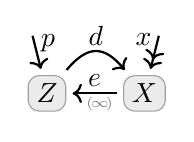
\begin{tikzpicture}
		[baseline=1.5ex]
		% [baseline=2.1ex]
		% [center base]
		\node[dpad0] (Z) {$Z$};
		\node[dpad0,right=.7 of Z] (X) {$X$};
		\draw[arr2, ->] (X) to[bend left=0]
			node[above, inner sep=2pt]{$e$}
			node[below, inner sep=1pt, pos=0.4]
				{${\color{gray}\scriptscriptstyle(\!\infty\!)}$}
			(Z);
		\draw[arr2, ->] (Z) to[bend left=50,looseness=1.5]
			% node[above]{$d$} (X);
			node[above, inner sep=2pt]{$\smash{d}$} (X);
		\draw[arr2, <<-] (X) --
			% node[above,pos=0.8]{$x$} ++(0.9, 0);
			node[left,pos=0.8,inner sep=2pt]{$x$} ++(0.2, 0.8);
		\draw[arr2, <-] (Z) --
			% node[left,pos=0.6,inner sep=2pt]{$p$} ++(-0.2, 0.8);%
			node[right,pos=0.7,inner sep=2pt]{$p$} ++(-0.2, 0.8);%
   \end{tikzpicture}$\mkern-1mu$}
   % \\&\qquad
   \!=\! \shortminus\!\mathop{\mathrm{E\mskip-0.5muL\mskip-0.6muB\mskip-0.7muO}}\limits_{p,e,d}\mskip-0.2mu(\mskip-1.5mux\mskip-1.5mu).
\end{align*}

The first and last equalities are \Cref{prop:marginal-ll,prop:pdg-elbo-vae}, and the inequality is \cref{lemma!}.
% Here $\Pr(X)$ is the marginal of $p(Z)d(X | Z)$ on $X$.
% The appendix contains multi-sample analogs of both propositions and the bound.
% See the appendix for multi-sample analogs of the bound and both propositions.
% See the appendix for multi-sample analogs of the bound and \cref{prop:pdg-elbo-vae}.
% For multi-sample analogs of the bound and \cref{prop:pdg-elbo-vae}, see the appendix.
See the appendix for multi-sample analogs of the bound and \cref{prop:pdg-elbo-vae}.
% See the appendix for multi-sample analogs of the bound and \cref{prop:pdg-elbo-x,prop:pdg-elbo-vae}.
% We give multi-sample analogs of both propositions and the bound in the appendix.

\subsection{The \texorpdfstring{$\beta$}{beta}-VAE Objective}
\label{sec:betavae}

The ELBO is not the only objective that has been used to train networks with a VAE structure.
% In the most common variant, \textcite{higgins2016beta} argue that one might want to weight the reconstruction error \eqref{eq:rec} and the KL term differently.  They suggest an objective of the form
In the most common variant, due to \textcite{higgins2016beta},
one weights the reconstruction error \eqref{eq:rec} and
% the KL term
the `KL term' differently, resulting in a loss function of the form
% \vskip-3ex
\vspace{-0.5ex}
\[
	\beta\text{-}\mathrm{ELBO}_{p,e,d}(x) := - \mathrm{Rec}(x) - \beta \kldiv{e(Z|x)}{p},
\]
% \vspace{-2ex}
\vskip-1.5ex
which, when $\beta \!=\! 1$, is the ELBO as before. The authors view $\beta$ as a regularization strength, and argue that
% in some cases, you can do better with a stronger prior.
% it helps to have a stronger prior in some cases.
% sometimes helps to put more stock in the prior.
it sometimes helps to have a stronger prior.
% sometimes helps to put more value in the prior.
Sure enough:
%oli3: add proposition
% Sure enough,
% the $\beta$-VAE objective is the inconsistency of the same
% PDG as before, but with confidence $\beta$ in $p(Z)$.%
\vspace{-2ex}
\begin{linked}{prop}{prop:betaelbo-informal}
\!\!$-\beta\text{-ELBO}_{p,e,d}(x)$ is the inconsistency of
% the same PDG as before,
the same PDG,
but with confidence $\beta$ in $p(Z)$.%
	% \footnote{The two parameters even share a name, both coming from thermodynamic $\beta$ (inverse temperature).}
	%TODO can I get my footnote also???
	% \footnote{Both names originate in thermodynamic coldness $\beta$.}
	% \footnote{They even share a name due to a common origin: thermodynamic coldness $\beta$.}
\end{linked}


\section{FREE ENERGY AND INCONSISTENCY}
% The factors of a factor graph, which in isolation indicate relative probabilities.
A weighted factor graph $\Psi = (\phi_J, \theta_J)_{J \in \cal J}$, where each $\theta_J$ is a real-valued weight, $J$ is associated with a subset of variables $\mathbf X_J$, and  $\phi_J : \V(\mathbf X_J) \to \mathbb R$, determines a distribution by
\vskip-1.4em
\[
	% \Pr\nolimits_\Psi(\mat x) \propto \prod_{j \in J} \phi_j(\mat x_j)^{\theta_j}
	\Pr\nolimits_\Psi(\mat x) = \frac{1}{Z_\Psi} \prod_{J \in \cal J} \phi_J(\mat x_J)^{\theta_J}.
\]
\vskip-0.7em
% The normalization constant $Z_{\Psi}$, is given by
% The normalization constant is given by
% where
% \begin{equation*}
\(
	Z_{\Psi} % :=
\)
is the constant
$ \sum_{\mat x} \prod_{J \in \mathcal J} \phi_J(\mat x_J)^{\theta_J}$
required to normalize the distribution,
% \end{equation*}
%joe1: I can't parse the rest of this sentence
%oli1:
% and is known as the \emph{partition function}, and is computing it is
and is known as the \emph{partition function}. Computing $\log Z_\Psi$
% is intimately related to much of probabilistic inference in factor graphs \parencite{ma2013estimating}.
is intimately related to probabilistic inference in factor graphs \parencite{ma2013estimating}.
%oli2:
Following \textcite{richardson2020probabilistic},
let $\PDGof{\Psi}$ be the PDG with edges $\{ \raisebox{-0.3ex}{$\smash{\stackrel{J}{\rightarrow}}$} \mathbf X_J \}_{\mathcal J}$, cpds $p_J(\mathbf X_J) \propto \phi_J(\mathbf X_J)$, and weights
% $\alpha_J \!=\! \beta_J \!=\! \theta_J$.
$\alpha_J, \beta_J := \theta_J$%
% , so defined because
% .
. There, it is shown that
% following \textcite{richardson2020probabilistic},
% $\PDGof{\Psi}$ is so defined becuase $\bbr{\dg M}_1^* = \{ \Pr_\Psi \}$.
$\Pr_\Psi$ is the unique minimizer of $\bbr{\PDGof{\Psi}}_1$.
But what about the corresponding inconsistency, $\aar{\PDGof{\Psi}}_1$?

% If every factor is a cpd, and every variable is the target of at least one edge, then $Z_\Psi$ is at most 1,
% Assuming every factor is normalized and every variable is a target of at least one edge, then $Z_\Psi$ is at most 1,
% If every factor is normalized and every variable is an edge target,
If the factors are normalized and all variables are edge targets,
then $Z_\Psi \le 1$,
% so $-\log Z_\Psi$ is non-negative, and
% so $-\log Z_\Psi \ge 0$, and
so $\log \frac{1}{Z_\Psi} \ge 0$
%  measures how far away the product of factors is from being normalized.
measures how far the product of factors is from being a probability distribution.
% Thus, it is in some sense a measure of inconsistency of a factor graph.
% So it is in some sense a measure of the factor graph's inconsistency.
So in a sense, it measures $\Psi$'s inconsistency.
% So in a sense, it measures the inconsistency of $\Psi$.
% It turns out that this intuition coincides with our notion of 1-inconsistency.
% This sense is precisely PDG 1-inconsistency.

\begin{linked}{prop}{fg-inconsistency-is-partition-function}
	For all weighted factor graphs
	$\Psi$,
	% $\Psi = (\phi_J, \theta_J)_{J \in \cal J}$,
	% Then
	 we have that $\aar{\PDGof{\Psi}}_1 = - \log Z_{\Psi}$.
\end{linked}

% Outside of computer science, such factored exponential families form
% the mathematical backbone of statistical mechanics.
% % DONE reword
% In this setting, $- \log Z_{\Psi}$ is the Heimholtz free energy.
% The exponential families generated by weighted factor graphs
% The exponential families generated by factor graphs and their weights $\boldsymbol\theta$
The exponential families generated by weighted factor graphs
are a cornerstone of statistical mechanics, where $- \log Z_{\Psi}$ is known as the (Heimholz) free energy.
%TODO: ADD A SENTENCE
It is also an especially natural quantity to minimize:
the principle of
free-energy minimization has been enormously succesful in describing
of not only chemical and biological systems \parencite{chipot2007free}, but also cognitive ones \parencite{friston2009free}.
%DONE: CITATIONS
% Many thermodynamic quantities
% (e.g., as internal energy, free energy, pressure, volume, and entropy) can
% be obtained by taking various partial derivatives of $Z_\Psi$, and calculating the partition function is closely related to infering marginal distributions \cite{}.


% \section{A CONCRETE EXAMPLE}
% \section{KEEPING THINGS STRAIGHT}
% \section{COMPOSITE LOSS FUNCTIONS}
% \section{STITCHING STANDARD LOSSES TOGETHER}
% \section{DIVERGENCE FROM STANDARD PRACTICE: A CONCRETE EXAMPLE}
% \section{DIFFERENCES FROM STANDARD PRACTICE}
\section{BEYOND STANDARD LOSSES: A CONCRETE EXAMPLE}
	\label{sec:datsim}
% When a loss function is standard in some context, it is usually for good reason---but with enough moving parts, cobbling standards together may not be ideal.
% In contexts where a loss function is standard, it is usually for good reason---but with enough moving parts, cobbling standards together may not be ideal.
%
In contexts where a loss function is standard, it is usually for good reason---which is why we have focused on recovering standard losses.
% But does viewing loss as inconsistency give us anything new?
But most situations are non-standard, and even if they have standard sub-components, those components may interact with one another in more than one way. 
Correspondingly, there is generally more than one way to cobble standard loss functions together. 
How should you choose between them? 
By giving a principled model of the situation. 
% This is the real power of our approach. 

\def\simsymb{\texttt{s\kern-1.1pti\kern-0.8ptm}}
\def\datsymb{\texttt{d\kern-0.75pta\kern-1ptt}}
\def\ssymb{\texttt{s}}
\def\dsymb{\texttt{d}}
% But sometimes, the standard  loss is used in a different context.
Suppose we want to train a predictor network $h(Y|X)$ from two sources of information:
% partially corrupted data with emperical distribution $d(X,Y)$,
partially corrupted data with distribution $d(X,Y)$,
and a simulation with distribution $s(X,Y)$.
If the simulation is excellent and the data unsalvagable, we would have high confidence in $s$ and low confidence in $d$, 
% which corresponds to training with cross entropy from $s$%
in which case we would train with cross entropy with respect to $s$%
% (i.e., $-\Ex_s \log h(Y|X)$).
% , $\Ex_s [\log \nf1{h(Y|X)}]$.
, $\mathcal L_{\simsymb}\!:=\!\Ex_s [\log \nf1{h(Y|X)}]$.
% Conversely, we would use
% % cross entropy from $d$, $\mathcal L_{\datsymb}\!:=\!\Ex_d [\log \nf1{h(Y|X)}]$
% $\mathcal L_{\datsymb}\!:=\!\Ex_d [\log \nf1{h(Y|X)}]$
% % if the simulation were bad and the data mostly intact.
% were the simulation bad and the data mostly intact.
% What if we're not so confident in either?
Conversely, if the simulation were bad and the data mostly intact, we would use
% cross entropy from $d$, $\mathcal L_{\datsymb}\!:=\!\Ex_d [\log \nf1{h(Y|X)}]$
$\mathcal L_\datsymb$,
the cross entropy with respect to $d$.
% $\mathcal L_{\datsymb}\!:=\!\Ex_d [\log \nf1{h(Y|X)}]$.
% cross entropy $\mathcal L_\datsymb$ from $d$.
% $\mathcal L_{\datsymb}\!:=\!\Ex_d [\log \nf1{h(Y|X)}]$
% if the simulation were bad and the data mostly intact.
What if we're not so confident in either?
% What if neither is strictly better than the other?

% \textbf{Backwards.}
One approach a practitioner might find attractive is to make a dataset from samples of both $s$ and $d$%
% (from $\lambda_s N$, $\lambda_d N$ samples),
, or equivalently, train with a convex combination
% $\mathcal L_1 := \lambda_0 \Ex_{s} \log \nf{1}{h(Y|X)} + \lambda_1 \Ex_{d} \nf{1}{ \log h(Y|X)}$
of the two previous losses,
$\mathcal L_1 := \lambda_{\ssymb}\mathcal L_{\simsymb} + \lambda_{\dsymb}\mathcal L_{\datsymb}$
% for some $\lambda_\ssymb, \lambda_\dsymb > 0$.
for some $\lambda_\ssymb, \lambda_\dsymb > 0$ with $\lambda_\ssymb + \lambda_\dsymb = 1$.
This amounts to training $h$ with cross entropy with respect to the mixture
% $\lambda_0 s + \lambda_1 d$.
$\lambda_\ssymb s + \lambda_\dsymb d$.
Doing so treats $d$ and $s$ as completely unrelated, and so redundancy is not used to correct errors---a fact on display when we present the modeling choices in PDG form, 
% such as $\mathcal L_1 = \aar{\dg M_1}$, where
such as
\vspace{-1ex}
\[
% \dg M_1 := ~
\mathcal L_1 = \aar**{
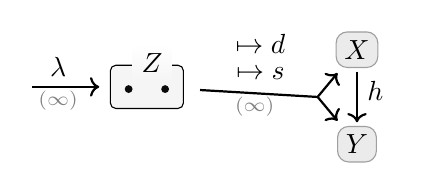
\begin{tikzpicture}[center base]
	% \node[dpad0] (Z) at (-0.2,0) {$Z$};
	% \node[tpt={z0|$0$}] at (-0.5,0.1) {};
	% \node[tpt={z1|$1$},right=0.15 of z0]{};
	\node[tpt={z0|\simsymb}] at (-0.5,0.1) {};
	\node[tpt={z1|\datsymb},right=0.35 of z0]{};
	\node[Dom={$Z$[label distance=-2.5ex, xshift=1.0em] (Z)
		around {\lab{z0}\lab{z1}}},yshift=0.2em ] {};

	% \node[dpad0,align=center] (XY) at (1.8,0) {$XY$}; %{$X$\\[-0.3ex]$Y$};
	\node[dpad0] (X) at (2.4, 0.6) {$X$};
	\node[dpad0] (Y) at (2.4, -0.6) {$Y$};
	\coordinate (xyz) at (1.9, 0);
	\draw[arr1, <-] (Z) to
		% node[above, pos=0.6]{$\hat\lambda$}
		node[above, pos=0.6]{$\lambda$}
		% node[above, pos=0.6]{$\frac{1}{\lambda_0+\lambda_1}[\lambda_0, \lambda_1]$}
		node[below,inner sep=1pt, pos=0.6]{${\color{gray}\scriptstyle( \infty )}$}
		+(-1.5, 0);
	% \node at (-1,-0.6) {\small where $\lambda(Z) = \frac{\lambda_Z}{\lambda_0+\lambda_1}$};
	% \node at (0,-0.6) {\small where $\lambda(Z) \propto \lambda_Z$};
	\draw[arr1] (X) to node[right,pos=0.4]{$h$} (Y);
	\draw[arr,-,shorten >=0pt] (Z) to[bend left=0, shorten >=0pt]
		% node[fill=white, inner sep=0pt, pos=0.55]
		% node[inner sep=1pt, pos=0.55]
		node[above, inner sep=1pt, pos=0.55]
			% {$Z?d:s$}
		% {$\begin{bmatrix}d \text{ if } Z\\[-0.3ex] s \text{ else}\end{bmatrix}$}
		% {$\begin{matrix}d \text{ if } Z\!\!=\!\!1\\[-0.3ex]
		% 	% s \text{ else}\end{matrix}$}
		% 	\text{else }s\end{matrix}$}
		{$\begin{matrix}\datsymb \mapsto d \\[-0.6ex]
			\simsymb \mapsto s \end{matrix}$}
		% node[above, inner sep=2pt, pos=0.68]
		% 	{${\color{gray}\scriptscriptstyle(r)}$}
		node[below,inner sep=1pt]{${\color{gray}\scriptstyle( \infty )}$}
		(xyz);
	\draw[arr2, shorten <=0pt] (xyz) to (X);
	\draw[arr2, shorten <=0pt] (xyz) to (Y);
\end{tikzpicture}}
	% (\lambda_\ssymb+\lambda_\dsymb),
	,
\]
% with probability $\lambda(Z) := \frac{1}{\lambda_0\!+\!\lambda_1}[\substack{\lambda_0\\\lambda_1}]$.
% with respective probabilities $\lambda(Z\!=\!0) = \frac{\lambda_0}{\lambda_0 + \lambda_1}$ and
% In $\dg M_1$, the swich variable $Z$ changes whether samples come from $s$ or $d$
% with respective probabilities $\lambda(Z\!=\!\simsymb) = \frac{\lambda_\ssymb}{\lambda_\ssymb + \lambda_\dsymb}$ and
% $\lambda(Z\!=\!\datsymb) = \frac{\lambda_\dsymb}{\lambda_\ssymb + \lambda_\dsymb}$.
% in which a swich variable $Z$ controls whether samples come from $s$ or $d$
% with respective probabilities $\lambda(Z\!=\!\simsymb) = \frac{\lambda_\ssymb}{\lambda_\ssymb + \lambda_\dsymb}$ and
% $\lambda(Z\!=\!\datsymb) = \frac{\lambda_\dsymb}{\lambda_\ssymb + \lambda_\dsymb}$.
in which a swich variable $Z$ 
with possible values
$
% \V(Z) :=
\{\simsymb,\datsymb\}$
controls whether samples come from $s$ or $d$, and 
is distributed according to
% $\lambda(Z\!=\!\simsymb) = \frac{\lambda_\ssymb}{\lambda_\ssymb + \lambda_\dsymb}$.
$\lambda(Z\!=\!\simsymb) = \lambda_\ssymb$.


% A second approach: use something like
% % $\mathcal L = \sum_{x\sim } h(y|x) \log \frac{h(y|x)}{d(y|x) q(y|x)}$
% $\smash{\Ex_{x\sim m} h(y|x) \log \frac{h(y|x)}{d(y|x) q(y|x)}}$.
Our practitioner now tries a different approach: draw data samples $(x,y) \sim d$ but discount $h$'s surprisal when the simulator finds the point unlikely, via loss $\mathcal L_2 := \Ex_{d} [s(\mkern-2muX\!,\!Y\mkern-2mu) \log \nf1{h(Y|X)}]$.
This is the cross entropy with respect to the (unnormalized) product density $ds$, which in many ways is appropriate.
However, by this metric, the optimal predictor $h^*(Y|x) \propto d(Y|x) s(Y|x)$ is
% uncalibrated
\emph{uncalibrated} \parencite{dawid1982well}.
% which means it is \emph{calibrated} \parencite{dawid1982well}.
If the data and simulator agree ($d \!=\! s$), then we would want $h(Y|x) \!=\! s(Y|x)$ for all $x$, but instead we get $h^*(Y|x) \propto s(Y|x)^2$.
So $h^*$ is overconfident.
What went wrong?
% $\mathcal L_2$ is not easily written as a (quantitative) inconsistency,
$\mathcal L_2$ cannot be written as a (purely quantitative) inconsistency
of a PDG containing only $s,h$, and $d$, 
but for a large fixed $\gamma$, it is essentially the $\gamma$-inconsistency
% but using the factor graph correspondence, it can be written as the 1-inconsistency
% $\mathcal L_2$ cannot be written as an inconsistency unless we also take the quailtative score into account, in which case it equals $\aar{\dg M_2}_1$.
% $\aar{\dg M_2 \text{ with } \alpha_d,\alpha_s \!:=\!1;~\alpha_h\!:=\!0}_1$.
% $\aar{\dg M_2 \text{ with } \alpha_d,\alpha_s \!:=\!1;~\alpha_h\!:=\!0}_1$.
% Although $\balpha$ is not the focus of the present paper, these values are problematic: they indicate an overdetermination of $X \times Y$, and as a consequence $h^*$ is more deterministic than it should be.
% The simplest PDG account of $\mathcal L_2$ is the 1-inconsistency 
% $\aar{ \dg M_2 }_1$,
% where
% \vspace{-2.5ex}
% \[
% % \dg M_2 :=
% \mathcal L_2 = 
% \lim_{k \to \infty}
% k
% \aar**{
% \begin{tikzpicture}[center base]
% 	\node[dpad0] (X) at (0, 0.6) {$X$};
% 	\node[dpad0] (Y) at (0, -0.6) {$Y$};
% 	\draw[arr1] (X) to node[left=0pt,pos=0.4, inner sep=1pt]{$h$}
% 			% node[below=0pt,inner sep=1pt,rotate=90]{${\color{gray}\scriptstyle(\!\alpha{:}0\!)}$}
% 			node[right=0pt,inner sep=1pt]{${\color{gray}\scriptstyle
% 				\renewcommand{\arraystretch}{.7}
% 				\big(\begin{matrix}
% 					\scriptstyle \alpha : 0 \\ \scriptstyle \beta : \frac1k
% 				\end{matrix}
% 				\big)}$}
% 		(Y);
% 
% 	\coordinate (d0) at (1.8, 0);
% 	\coordinate (dmid) at (0.9, 0);
% 	\coordinate (s0) at (-1.8, 0);
% 	\coordinate (smid) at (-0.9, 0);
% 	% \node[above left=1pt and 0.5em of d0] {$d$};
% 	% \node[below left=0pt and -1em of d0]{${\color{gray}\scriptstyle
% 	% 	\renewcommand{\arraystretch}{.8}
% 	% 	\begin{pmatrix} \scriptstyle\alpha: 1 \\[-0.2ex] \scriptstyle\beta:1 \end{pmatrix}}$};
% 	% \node[above right=1pt and 0.5em of s0] {$s$};
% 	% \node[below right=0pt and -1em of s0]{${\color{gray}\scriptstyle
% 	% 	\renewcommand{\arraystretch}{.8}
% 	% 	\begin{pmatrix}\scriptstyle
% 	% 	\alpha: 1 \\[-0.2ex] \scriptstyle \beta: 1 \end{pmatrix}}$};
% 
% 	% \unmergearr{s0}XY
% 	% \unmergearr{d0}XY
% 	\draw[arr,->,shorten <=0pt] (dmid) to[bend right=25] (X);
% 	\draw[arr,->,shorten <=0pt] (dmid) to[bend left=25] (Y);
% 	\draw[arr1,-,shorten <=0pt] (dmid) to
% 		node[below, inner sep=2pt]{${\color{gray}\scriptstyle
% 			\renewcommand{\arraystretch}{.7}
% 			\big(\begin{matrix}
% 				\scriptstyle\alpha: 1 \\[-0.2ex] \scriptstyle\beta:1
% 			\end{matrix} \big)}$}
% 		node[above] {$d$}
% 		(d0);
% 	%
% 	\draw[arr,->,shorten <=0pt] (smid) to[bend left=25] (X);
% 	\draw[arr,->,shorten <=0pt] (smid) to[bend right=25] (Y);
% 	\draw[arr1,-,shorten <=0pt] (smid) to
% 		node[below, inner sep=2pt]{${\color{gray}\scriptstyle
% 			\renewcommand{\arraystretch}{.7}
% 			\big( \begin{matrix}
% 				\scriptstyle \alpha: 1 \\[-0.2ex] \scriptstyle \beta: 1
% 			\end{matrix} \big)}$}
% 		node[above]{$s$}
% 		(s0);
% % 	\draw[arr,-,shorten >=0pt] (Z) to[bend left=0, shorten >=0pt]
% % 		node[fill=white, inner sep=0pt, pos=0.55]
% % 			% {$Z?d:s$}
% % 			{$\begin{bmatrix}d\\[-0.3ex] s\end{bmatrix}$}
% % 		% node[above, inner sep=2pt, pos=0.68]
% % 		% 	{${\color{gray}\scriptscriptstyle(r)}$}
% % 		(xyz);
% % 	\draw[arr2, shorten <=0pt] (xyz) to (X);
% % 	\draw[arr2, shorten <=0pt] (xyz) to (Y);
% % ode[dpad0] (X) {};
% \end{tikzpicture}}\Bigg._{\!\!1} - k \log C,
% \]
% \[
% % \dg M_2 :=
% \mathcal L_2 = 
% \lim_{k \to \infty}
% \aar**{
% \begin{tikzpicture}[center base]
% 	\node[dpad0] (X) at (0, 0.6) {$X$};
% 	\node[dpad0] (Y) at (0, -0.6) {$Y$};
% 	\draw[arr1] (X) to node[left=0pt,pos=0.4, inner sep=1pt]{$h$}
% 			% node[below=0pt,inner sep=1pt,rotate=90]{${\color{gray}\scriptstyle(\!\alpha{:}0\!)}$}
% 			node[right=0pt,inner sep=1pt]{${\color{gray}\scriptstyle
% 				\renewcommand{\arraystretch}{.7}
% 				\big(\begin{matrix}
% 					\scriptstyle \alpha : 0 \\ \scriptstyle \beta : 1
% 				\end{matrix}
% 				\big)}$}
% 		(Y);
% 
% 	\coordinate (d0) at (1.8, 0);
% 	\coordinate (dmid) at (0.9, 0);
% 	\coordinate (s0) at (-1.8, 0);
% 	\coordinate (smid) at (-0.9, 0);
% 
% 	\draw[arr,->,shorten <=0pt] (dmid) to[bend right=25] (X);
% 	\draw[arr,->,shorten <=0pt] (dmid) to[bend left=25] (Y);
% 	\draw[arr1,-,shorten <=0pt] (dmid) to
% 		node[below, inner sep=2pt]{${\color{gray}\scriptstyle
% 			\renewcommand{\arraystretch}{.7}
% 			\big(\begin{matrix}
% 				\scriptstyle\alpha: 1 \\[-0.2ex] \scriptstyle\beta:k
% 			\end{matrix} \big)}$}
% 		node[above] {$d$}
% 		(d0);
% 	%
% 	\draw[arr,->,shorten <=0pt] (smid) to[bend left=25] (X);
% 	\draw[arr,->,shorten <=0pt] (smid) to[bend right=25] (Y);
% 	\draw[arr1,-,shorten <=0pt] (smid) to
% 		node[below, inner sep=2pt]{${\color{gray}\scriptstyle
% 			\renewcommand{\arraystretch}{.7}
% 			\big( \begin{matrix}
% 				\scriptstyle \alpha: 1 \\[-0.2ex] \scriptstyle \beta: k
% 			\end{matrix} \big)}$}
% 		node[above]{$s$}
% 		(s0);
% 	\end{tikzpicture}}\Bigg._{\!\!k} - k \log C,
% \]
\[
% \dg M_2 :=
\mathcal L_2 \approx
C
\aar**{
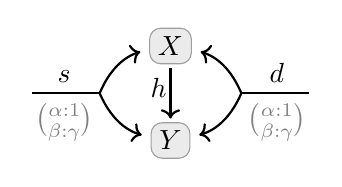
\begin{tikzpicture}[center base]
	\node[dpad0] (X) at (0, 0.6) {$X$};
	\node[dpad0] (Y) at (0, -0.6) {$Y$};
	\draw[arr1] (X) to node[left, pos=0.4, inner sep=1pt]{$h$}
			% node[below=0pt,inner sep=1pt,rotate=90]{${\color{gray}\scriptstyle(\!\alpha{:}0\!)}$}
			%oli: NO NEED!
			% node[right=0pt,inner sep=1pt]{${\color{gray}\scriptstyle
			% 	\renewcommand{\arraystretch}{.7}
			% 	\big(\begin{matrix}
			% 		\scriptstyle \alpha : 0 \\ \scriptstyle \beta : 1
			% 	\end{matrix}
			% 	\big)}$}
		(Y);

	\coordinate (d0) at (1.8, 0);
	\coordinate (dmid) at (0.9, 0);
	\coordinate (s0) at (-1.8, 0);
	\coordinate (smid) at (-0.9, 0);
	
	\draw[arr,->,shorten <=0pt] (dmid) to[bend right=25] (X);
	\draw[arr,->,shorten <=0pt] (dmid) to[bend left=25] (Y);
	\draw[arr1,-,shorten <=0pt] (dmid) to
		node[below, inner sep=2pt]{${\color{gray}\scriptstyle
			\renewcommand{\arraystretch}{.7}
			\big(\begin{matrix}
				\scriptstyle\alpha: 1 \\[-0.2ex] \scriptstyle\beta: \gamma
			\end{matrix} \big)}$}
		node[above] {$d$}
		(d0);
	%
	\draw[arr,->,shorten <=0pt] (smid) to[bend left=25] (X);
	\draw[arr,->,shorten <=0pt] (smid) to[bend right=25] (Y);
	\draw[arr1,-,shorten <=0pt] (smid) to
		node[below, inner sep=2pt]{${\color{gray}\scriptstyle
			\renewcommand{\arraystretch}{.7}
			\big( \begin{matrix}
				\scriptstyle \alpha: 1 \\[-0.2ex] \scriptstyle \beta: \gamma
			\end{matrix} \big)}$}
		node[above]{$s$}
		(s0);
\end{tikzpicture}}\Bigg._{\!\!\!\gamma}
% - k \log Z_{sd} + H
% - k \log C,
 + \mathit{const},
% \overbrace{ - k \log C, }^{\text{normalization constant for $sd$}}
\]
where $C$ is the constant required to normalize the joint density $sd$, and $\mathit{const}$ does not depend on $h$. 
However, the values of $\balpha$ in
this PDG indicate an over-determination of $XY$
% (it is determined in two ways),
(it is determined in two different ways),
  % and so $h^*$ is more deterministic than it should be.
  and so $h^*$ is more deterministic than intended.
By contrast, 
% $\aar{\dg M_3}$
\vspace{-2ex}
\[
% \dg M_3 :=
\mathcal L_3 := \aar**{
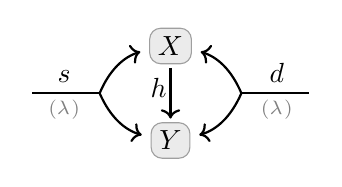
\begin{tikzpicture}[center base]
	\node[dpad0] (X) at (0, 0.6) {$X$};
	\node[dpad0] (Y) at (0, -0.6) {$Y$};
	\draw[arr1] (X) to node[left=0pt,pos=0.4, inner sep=1pt]{$h$} (Y);

	% \coordinate (d0) at (1.3, 0);
	% \coordinate (s0) at (-1.3, 0);
	% \node[above left=1pt and 0.5em of d0] {$d$};
	% \node[below left=0pt and 0.2em of d0]{${\color{gray}\scriptstyle( \lambda_1 )}$};
	% \node[above right=1pt and 0.5em of s0] {$s$};
	% \node[below right=0pt and 0.2em of s0]{${\color{gray}\scriptstyle( \lambda_0 )}$};

	\coordinate (d0) at (1.8, 0);
	\coordinate (dmid) at (0.9, 0);
	\coordinate (s0) at (-1.8, 0);
	\coordinate (smid) at (-0.9, 0);
	
	\draw[arr,->,shorten <=0pt] (dmid) to[bend right=25] (X);
	\draw[arr,->,shorten <=0pt] (dmid) to[bend left=25] (Y);
	\draw[arr1,-,shorten <=0pt] (dmid) to
		node[below, inner sep=2pt]{${\color{gray}\scriptstyle(\lambda_{\dsymb})}$}
		node[above] {$d$}
		(d0);
	%
	\draw[arr,->,shorten <=0pt] (smid) to[bend left=25] (X);
	\draw[arr,->,shorten <=0pt] (smid) to[bend right=25] (Y);
	\draw[arr1,-,shorten <=0pt] (smid) to
		node[below, inner sep=2pt]{${\color{gray}\scriptstyle(\lambda_{\ssymb})}$}
		node[above]{$s$}
		(s0);
	% \unmergearr{s0}XY
	% \unmergearr{d0}XY
% 	\draw[arr,-,shorten >=0pt] (Z) to[bend left=0, shorten >=0pt]
% 		node[fill=white, inner sep=0pt, pos=0.55]
% 			% {$Z?d:s$}
% 			{$\begin{bmatrix}d\\[-0.3ex] s\end{bmatrix}$}
% 		% node[above, inner sep=2pt, pos=0.68]
% 		% 	{${\color{gray}\scriptscriptstyle(r)}$}
% 		(xyz);
% 	\draw[arr2, shorten <=0pt] (xyz) to (X);
% 	\draw[arr2, shorten <=0pt] (xyz) to (Y);
% ode[dpad0] (X) {};
\end{tikzpicture}},
\]
% although complicated in closed form,
% \vspace{-2ex}
does not have this issue: the optimal predictor $h^*$
 % by this metric
 according to $\mathcal L_3$
 is proportional to the $\lambda$-weighted geometric mean of $s$ and $d$.
% Both losses of the initial approach also arise from PDGs, and the lack of calibration in the second stems from strange modeling assumptions.
% The discussion at the end of \S8 and Appendix C.1.2 gives another calibration example.
% We will add this example to the appendix as well.
% This example addresses Reviewer \#3's concern: thinking about what's going on is more than pedagogy; it is a valuable first step in the modeling workflow!
% For \revc{Reviewer \#4}: viewing losses through the same lens like this makes it possible to analyze and choose loss functions uniformly, as we say in the introduction.
% To address \revc{Reviewer #3}: this ; describing what's going on is a valuable safeguard first step in the modeling workflow.
% So, in addition to this unified view of standard loss functions, our approach can suggest more appropriate loss functions for non-standard situations.
% We submit that, in addition to providing a unified view of standard loss functions, our approach can suggest more appropriate loss functions in practical problems.
It seems that our approach, in addition to providing a unified view of standard loss functions, can also suggest more appropriate loss functions in practical situations.

% \section{COST AS INCONSISTENCY?}
% \section{R\kern-0.04emE\kern-0.07emV\kern-0.05emERSE-EN\kern-0.07emG\kern-0.05emINEERIN\kern-0.07emG A L\kern-0.05emO\kern-0.02emSS}
% \section{R\kern-0.04emE\kern-0.07emV\kern-0.05emERSE-EN\kern-0.07emG\kern-0.05emINEER A L\kern-0.05emO\kern-0.02emSS?}
% \section{R\kern-0.04emE\kern-0.07emV\kern-0.05emERSE-EN\kern-0.07emG\kern-0.05emINEERIN\kern-0.07emG L\kern-0.05emO\kern-0.02emSSES} %% TOO LONG
% \section{ON R\kern-0.04emE\kern-0.07emV\kern-0.05emERSE-EN\kern-0.07emG\kern-0.05emINEERIN\kern-0.07emG}
% \section{R\kern-0.04emE\kern-0.07emV\kern-0.05emER\kern-0.03emS\kern-0.03emE-EN\kern-0.07emG\kern-0.05emINE\kern-0.03emERIN\kern-0.07emG \kern-0.07emA \kern-0.07em L\kern-0.05emO\kern-0.02emS\kern-0.05emS?}%% Can't get it to work. TOO long.
\section{REVERSE-ENGINEERING LOSS?}
% \section{REVERSE-ENGINEERING A LOSS FUNCTION?}
% \section{ON WORKING BACKWARDS}
% \section{ON WORKING BACKWARDS FROM LOSS}
% \section{REVERSE ENGINEERING LOSSES}
	\label{sec:reverse-engineer}

\def\Truth{{\tt T}}
\def\trut{{\tt t}}
\def\truf{{\tt f}}

% Is it possible to get \emph{every} expression out of the inconsistency?
% Is it possible to make an arbitrary loss function  $\ell(X)$ appear as an inconsistency?
% Is it possible to make an arbitrary loss function appear as an inconsistency?
% Given an arbitrary loss function $\ell(X)$, can we find a PDG that gives rise to it?
% Given an arbitrary loss function $\ell(X)$, is there an algorithm to find a PDG that gives rise to it?
% Given an arbitrary loss function $\ell(X)$, can we find a PDG that gives rise to it?
Given an arbitrary loss function, can we find a PDG that gives rise to it?
% To a first approximation, it may seem that the answer is yes.
% To a first approximation, the answer seems to be yes.
%% TODO
% Not in a satisfying way, although at first glance, the answer appears to be yes.
At first glance, the answer appears to be yes.
% To a first approximation, the answer appears to be yes.
%
% Just as including probabilistic information is not a matter of multiplication, inconsistency is not a mere matter of addition.
%
%
% ABORT
% We promised a ``universal'' loss function.
% When we promised a ``universal'' loss function, we meant that we had a single function that works in all scenarios, not that it could turn into any loss.
% We have delivered one that is a relatively choiceless, universal construction.
%
% One can add the variable $\Truth$, whose values are $\{\trut, \truf\}$, and the event $\Truth \!\!=\! \trut$, to any PDG without affecting its semantics.
Without affecting its semantics, one may add the variable $\Truth$ that takes values $\{\trut, \truf\}$, and the event $\Truth \!\!=\! \trut$, to any PDG.
% Without affecting its semantics, one may add to any PDG the variable $\Truth$ that takes values $\{\trut, \truf\}$, and the event $\Truth \!\!=\! \trut$.
%
% Now, given any non-negative function
Now, given a
cost function $c: \V(X) \to \mathbb R^{\ge 0}$,
% cost function $c(X) \ge 0$,
% non-negative cost function,
% function $f(X)$,
define the cpd $\hat c(\Truth |X)$ by
$
	\hat c(\trut | x) := \exp( - c(x)).
$
% $\hat c$ ties the value of $X$ to inconsistency by threatening to generate the falsehood {\tt f}, with probability dependent on the cost of $X$.
% By threatening to generate the falsehood {\tt f}, in proporition to the cost of $X$, $\hat c$ ties the value of $X$ to inconsistency.
% By threatening to generate the falsehood {\tt f}, with probability dependent on the cost of $X$, $\hat c$ ties the value of $X$ to inconsistency.
By threatening to generate the falsehood {\tt f} with probability dependent on the cost of $X$, $\hat c$ ties the value of $X$ to inconsistency.
% So $\aar{\!\begin{tikzpicture}[center base]
% 			\node[dpadinline] (X) at (0,0) {$X$};
% 			\node[dpadinline] (2) at (1.1,0) {$\Truth$};
%
% 			\draw[arr2] (X) to
% 				node[above, pos=0.4,inner sep=2pt]{$\hat c$}
% 				% node[below, pos=0.4, inner sep=2pt]{${\color{gray}\scriptstyle(\beta)}$}
% 				(2);
% 			\draw[arr2, <<-] (X) to
% 				node[above, pos=0.6, inner sep=2pt]{$x$}
% 				% node[below, pos=0.6, inner sep=2pt]
% 					% {${\color{gray}\scriptscriptstyle(\mskip-2mu\infty\mskip-2mu)}$}
% 				+(-0.9, 0);
% 			\draw[arr2, <<-] (2) to
% 				node[above, inner sep=2pt, pos=0.6]
% 					{\trut}
% 				+(0.9,0);
% 		\end{tikzpicture}\!}
% 	 	= \!
% 		% \beta \Ex_{x\sim p}c(x).
% 		c(x)$, and
% \TODO
% \newpage
\begin{linked}{prop}{expected-cost}
	% Given a distribution $p(X)$ and a cost $c$,
	% \def\binvar{\mathbbm 2}
	% \[
	\!
	\( \displaystyle
		\aar*{\!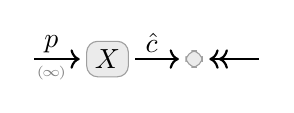
\begin{tikzpicture}[center base]
			\node[dpad0] (X) at (0,0) {$X$};
			\node[dpad0] (2) at (1.1,0) {$\Truth$};

			\draw[arr2] (X) to
				node[above, pos=0.4,inner sep=2pt]{$\hat c$}
				% node[below, pos=0.4, inner sep=2pt]{${\color{gray}\scriptstyle(\beta)}$}
				(2);
			\draw[arr2, <-] (X) to
				node[above, pos=0.6, inner sep=2pt]{$p$}
				node[below, pos=0.6, inner sep=2pt]
					{${\color{gray}\scriptscriptstyle(\mskip-2mu\infty\mskip-2mu)}$}
				+(-1, 0);
			\draw[arr2, <<-] (2) to
				node[above, inner sep=2pt, pos=0.6]
					{\trut}
				+(0.9,0);
		\end{tikzpicture}\!}
	 	= \!
		% \beta \Ex_{x\sim p}c(x).
		\Ex_{x\sim p}\! c(x).
	% \]
	\)
\end{linked}
% So \emph{every} cost function arises as an inconsistency.
% But it is still not possible to slap on loss functions without tyranical micromanagement.
% But it is still not easy to simply reverse-engineer functions without micromanagement bordering on tyrany.
% reverse-engineer PDGs from loss functions. ...
% But this trick is not enough to simply reverse-engineer loss functions and work with them as before.
% But we still can't simply
% But inconsistency is a global property: one cannot simply ``emit it'' and trust that it will collect additively; the PDG squirms and contorts to disperse it.
% Above, we had to set $\beta_p := \infty$.
% Above, setting $\beta_p := \infty$ was necessary.
% Setting $\beta_p := \infty$ above was necessary, for example.
% But inconsistency is a global property: one cannot simply ``emit it'' and trust that it will collect additively; the PDG squirms and contorts to disperse it.
% However, setting $\beta_p := \infty$ is necessary.
Setting confidence $\beta_p := \infty$ may not be realistic since
we're still training the model $p$,
% but it is necessary to recover $\Ex_p c$.%
but doing so is necessary to recover $\Ex_p c$.%
%$\ell$.
\footnote{If $\beta_p$ were instead equal to $1$, we would have obtained $-\log \Ex_p \exp(-c(\!X\!))$, with optimal distribution $\mu(\!X\!) \!\ne\! p(\!X\!)$.\label{fn:logEexp}}
% (  )
Any mechanism that generates inconsistency based on the value of $X$ (such as this one) also works in reverse:
% the PDG squirms, contorting the probability of $X$ to disperse the inconsistency.
the PDG ``squirms'', contorting the probability of $X$ to disperse the inconsistency.
% One cannot cannot simply ``emit'' inconsistency
One cannot cannot simply ``emit loss''
without affecting the probabilistic part of the model,
%oli3:
% as one does with value in an influence diagram \parencite{influencediagrams}.
as one does
% with ``value''
in an influence diagram \parencite{influencediagrams}
with value nodes.
%TODO CITE
% and expect to collect it
%
% additively without affecting the model.
% without affecting the optimal probabilities.
%
% In more complex settings, even setting every $\beta$ to $\infty$ may not be enough.
% In more complex settings, even setting every $\beta := \infty$ may not be enough to prevent the squirming.
Even setting every $\beta := \infty$ may not be enough to prevent the squirming.
% To illustrate, consider the following PDG $\dg{SL}$, which is
% a modification of the PDG in \Cref{prop:supervised-cross-entropy}
% the natural modification of the PDG in \Cref{prop:supervised-cross-entropy}
% To illustrate, consider the analogous modification of PDG in \Cref{prop:supervised-cross-entropy}, which models the setup of supervised learning with an arbitrary loss function $\ell$.
\def\mypdg{\dg{S}}
To illustrate, consider a model $\mypdg$ of the supervised learning setting (predict $Y$ from $X$), with labeled data $\mathcal D$, model $h$, and an arbitrary loss function $\ell$ on pairs of output labels.
 % Define:
Concretely, define:
\vspace{-1ex}
% \def\mypdg{\dg{S}\!\dg{L}}
% \def\mypdg{\dg{S}\!\mathrm{Learn}}
\[
	\mypdg
	:=
	% \aar*{
	\begin{tikzpicture}[baseline=4ex]
		\begin{scope}[xscale=1.2]
			\node[dpad0] (X) at (0.3,0) {$X$};
			\node[dpad0] (Yt) at (1,1) {$Y$};
			% \node[dpad0,align=center] (Yp) at (1,0) {$\vphantom{Y}\smash{\hat Y}$};
			% \node[dpad0,align=center] (Yp) at (1,0) {$\vphantom{Y}\smash{Y'}$};
			\node[dpad0,align=center] (Yp) at (1.4,0) {$\vphantom{Y}\smash{Y'}$};
			\node[dpad0] (2) at (2,1) {$\Truth$};

			\coordinate (dstart) at (-0.1,0.9);
			% \coordinate (tstart) at (2,0.9);
		\end{scope}

		% \draw[arr2] (X) to
		% 	node[above, pos=0.4,inner sep=2pt]{$\tilde c$}
		% 	node[below, pos=0.4, inner sep=2pt]{${\color{gray}\scriptstyle(\beta)}$}
		% 	(2);
		% \draw[arr2, <-] (X) to
		% 	node[above, pos=0.6, inner sep=2pt]{$p$}
		% 	node[below, pos=0.6, inner sep=2pt]{${\color{gray}\scriptstyle(\infty)}$}
		% 	+(-1, 0);
		\unmergearr[arr1]{dstart}{X}{Yt}
			\node[above=2pt of center-dstartXYt, xshift=-2pt] {$\datadist\xysamp$};
			\node[below right=2.0pt and -0.4pt of center-dstartXYt, inner sep=0pt, rotate=25]
				{${\color{gray}\scriptscriptstyle(\mskip-2mu\infty\mskip-2mu)}$};

		\mergearr[arr2]{Yt}{Yp}{2}
			\node[above=2pt of center-YtYp2] {$\hat\ell$};

		\draw[arr2] (X) to
			node[above, inner sep=2pt,pos=0.4] {$h$}
			node[below, inner sep=2pt,pos=0.4]
				{${\color{gray}\scriptscriptstyle(\mskip-2mu\infty\mskip-2mu)}$}
			(Yp);
		\draw[arr2, <<-] (2) to
			node[right, inner sep=2pt, pos=0.6]
				{\trut}
			% +(0,1);
			+(0,-1);
	\end{tikzpicture}
	% }
	% = \beta \Ex_{x\sim p}c(x).
	\quad\;\text{and}\;\quad
	% L := \Ex_{x,y\sim \mathcal D}\Ex_{y' \sim p|x}\ell(y,y')
	\mathcal L := \;\;\mathop{\scalebox{1.2}{$\Ex$}}\limits_{\substack{%
		\vphantom{x}\\
		\mathllap{(x,y)} \sim \mathrlap{\datadist\xysamp} \\
		\mathllap{y'} \sim \mathrlap{p(Y'|\,x)}} }
	 \;\big[\ell(y,y')\big].
	 %
	 \vspace{-1.5ex}
\]

%TODO
% You might think after seeing Prop 14: "why bother with PDGs if they don't even have bite?
% I can model whatever I want with loss functions directly and  then have my secretary convert
% them to PDGs. It doesn't change the way that I think, like a good programming language should".
%
% But this is not the case --- if you generate inconsistency conditioned on Y and Y', the rest of the PDG will react to it, and bend so that Y and Y' exhibit more favorable behavior.
%
% The point:
% If there are some moving parts, you have to go way out of your way to nail them down.
% In many cases, you will need to enforce independence, at which point
% you have no choice but to use $\gamma$ or send an \alpha to -\infty, either coopting global properties,
% or bending the definition for a strange anti-causal parameter.
%
% You might think this will simply give you expected loss here, but it does not. It gives you something better.
%varsha:
% \textbf{Punchline}:
% \TODO[PUNCHLINE: it's not enough.]
%
%
Given \Cref{prop:expected-cost},
one might imagine $\aar{\mypdg} = \mathcal L$,
% the expected classifier loss,
but this is not so.
% but we accidentally obtained something nicer.
% But $\aar{\mypdg}$ is arguably nicer.
In some ways, $\aar{\mypdg}$ is actually preferable.
% But $\aar{\mypdg}$ is not such a bad loss either.
% But perhaps we should not be so quick to write off $\aar{\mypdg}$.
% Although we should not be so quick to overlook $\aar{\mypdg}$.
% the optimal $p(Y|X)$ by minimizing $L$ is a point mass on the label $y^*_X$ that minimizes expected loss given $X$, but the optimal $p(Y|X)$ according to $\aar{\mypdg}$ is $\datadist\xysamp(Y|X)$,%
% \footnote{assuming $\ell(y,y') \ge 0$ with equality iff $y=y'$}
%
The optimal $h(Y'|X)$ according to $\mathcal L$ is
% a point mass on the label $y^*_X$ minimizing expected loss,
a degenerate cpd that places all mass on the label $y^*_X$ minimizing expected loss,
while the optimal $h(Y'|X)$ according to $\aar{\mypdg}$ is $\datadist\xysamp(Y|X)$,
	% \footnote{assuming $\ell(y,y') \ge 0$ with equality iff $y=y'$}
% which means it is \emph{calibrated} \parencite{dawid1982well}.
which means that, unlike $\ell$, it is calibrated.
If, in addition, we set $\alpha_p, \alpha_{\datadist\xysamp} := 1$ and strictly enforce the qualitative picture,
finally no more squirming is possible, as we arrive at
	% \footnote{which means also setting $\alpha_p, \alpha_{\datadist\xysamp} := 1$}
% we still get $L = \aar{\mypdg}_\infty$.
$\displaystyle\lim_{\gamma\to\infty}\aar{\mypdg}_\gamma = \mathcal L$.
% (see the appendix.)
\vspace{-0.5ex}

% But now we've roped in the global parameter $\gamma$. 
%TODO Add sentence 
% But now 
% But now we've roped in the global parameter $\gamma$
% But now we've maxed out on inconsistency; 
% To summarize, working backwards requires indicating absolute certainty in strange modeling assumptions.
% To summarize, working backwards requires making strange choices, and indicating absolute certainty in them.
To summarize: 
% while 
% while going from model to loss function 
% while going from model to loss function seems to give the right loss function at every turn, generalizing properly to new information,
% working backwards requires nailing down behavior with absolute certainty, so that it does not change in response to your loss.
% reverse-engineering a loss function is possible, but requires making all modeling choices with absolute certainty, including some questionable ones.
% working backwards from loss to PDG is possible, but requires indicating absolute certainty in all modeling choices, including some questionable ones.
working backwards from loss to PDG, although possible, may require reporting absolute certainty in all modeling choices, including some questionable ones.
% This leaves zero margin for error.
% indicating absolute certainty in them.
In the end, we must confront our modeling choices;
good loss functions come from good models.
% good loss functions come from good models, and not the other way around.
% In the end, we must all confront our modeling choices; the only difference here is that they are on display.
% Good loss functions come from good models.

% Good loss functions come from good models, and you will be hard pressed to explain assumptions if you work like this.
%
% Working in this way is possible, but requires a tyrnanical level of micromanagement.
% When all is said and done, we must then confront our modeling assumptions. Why do you believe the cpd $\hat \ell$? What does it mean?
% And what's wrong with the simpler model without $\hat\ell$ or $\Truth$ when $Y = Y'$, which gives us cross entropy?
%
% In the PDG world, you get nice things by default, and have to make bad modeling assumptions to reduce it to what you had before.
%
%
% Varhsa:
% Good loss functions come out of good models. Corresponding PDG will have hard to explain structure.
%
% What's going on here?
% It is impossible to specify a cost
% without affecting internal infemum of the inconsistency.
%
% \begin{linked}{prop}{loss-into-pdg}
% 	% \def\binvar{\mathbbm 2}
% 	% \def\binvar{B}
% 	% Given a cost function $c: \V(X) \to \mathbb R_{\ge 0}$ and distribution $p(X)$,
% 	% let $\binvar$ be a fresh binary variable, and define $\tilde c(\binvar |X)$ by
% 	% $
% 	% 	\tilde c(\binvar\!\!=\!\!1 | X) := \exp(- c(X)).
% 	% $
% 	Then,
%
% 	\begin{align*}
% 		\arg\min_{p}
% 		\aar[\Big]{\mathop{\mypdg}\limits_{p,\xysamp, \ell}}_0 &=
% 		 	\datadist\xysamp(Y|X)
% 		\\%
% 		\lim_{\gamma \to \infty} \arg\min_{p}
% 		\aar[\Big]{\mathop{\mypdg}\limits_{p,\xysamp, \ell}}_{\!\gamma} &=
% 			\delta_{y^*_X}(Y|X)
% 			% [\arg\max_y \datadist\xysamp(y|X)]
% 	\end{align*}
% 	where $y^*_X := \arg\min_{y} \Ex_{y' \sim \datadist\xsamp(Y|X)}\ell(y,y')$ is the maximum likelihood label given $X$ and $\delta_{y^*_X}(Y|X)$ is the point mass on it.
% \end{linked}
% So,
%
%TODO
% Yeah sure you can get any loss function but if you look at the corresponding PDG it makes no sense


\section{FINAL REMARKS}

% TODO
% Varsha says: punchline is missing
% not clear that you should use this to check your modeling assumptions

% We have now seen that PDG semantics not only capture structured objects such as Bayesian Networks and Factor Graphs as in \textcite{richardson2020probabilistic},
% but in the same stroke also generate
%TODO
%joe2: replace with
% but also can be used to generate
% but in the same stroke also generate
% but the same  
% We have now seen that PDG semantics, not only capture structured models such as Bayesian Networks and Factor Graphs as in \textcite{richardson2020probabilistic}, but also, in the same stroke generate
% We seen that that PDG semantics, in the same stroke by which they capture Bayesian Networks and Factor Graphs, also generate
We seen that that PDG semantics, in the same stroke by which they capture Bayesian Networks and Factor Graphs \parencite{richardson2020probabilistic}, also generate
%
% many standard loss functions, including some non-trivial ones.
many standard loss functions, including some non-trivial ones.
% In each case, the appropriate loss is a simple consequence of carefully articulating modeling assumptions.
% In each case, the appropriate loss arises simply by articulating modeling assumptions, and then measuring the inconsistency of the resulting model.
In each case, the appropriate loss arises simply by articulating modeling assumptions, and then measuring inconsistency.
Viewing loss functions in this way also has beneficial side effects, including an intuitive visual proof language for reasoning about the relationships between them.

%joe1*: I *strongly* suggest removing this paragraph.   You have
%provided no evidence whatsoever that what you are doing is in the
%spirit of cognitive dissonance (which is about how an agent handles
%conflicting beliefs, largely by ignoring upsetting information).
% Taking a step back, we submit that this approach to modeling agents, which is similar in spirit to the theory of \emph{cognitive dissonance} \cite{}, is also more plausible for humans than one that supposes we minimize expectations of some concrete, exogenously given measure of (dis)utility.
% We also believe that our ``universal loss function'' will be of substantial interest to the AI safety community.
 % blurring the line between model and objective.
%
% This ``universal loss function'',
% which provides a principled way of choosing an optimization objective,
% % which blurs the line between model and objective function,
% may be of particular interest to the AI safety community.
This ``universal loss'',
which provides a principled way of choosing an optimization objective,
% which blurs the line between model and objective function,
% may be of particular interest to the AI safety community.
may be of particular interest to the AI alignment community.
% Taking a step back, we submit that this approach to modeling agents 


\newpage
\subsubsection*{Acknowledgements}
Work supported in part by MURI grant W911NF-19-1-0217. 
Many thanks to my advisor, Joe Halpern, for his generous support, and for valuable critiques of many drafts. Thanks as well to my reviewers, who pushed me to better explain the confidence parameters, and to include a practical example (\Cref{sec:datsim}).
Finally, thanks to my friends, particularly Varsha Kishore and Greg Yauney, for helping me to refine these ideas.

% All acknowledgments go at the end of the paper, including thanks to reviewers who gave useful comments, to colleagues who contributed to the ideas, and to funding agencies and corporate sponsors that provided financial support.
% To preserve the anonymity, please include acknowledgments \emph{only} in the camera-ready papers.


% \clearpage
\subsubsection*{References}
%joe1: lotys of problems here:
%- [8] and [9] are the same, mwention Mackay twice, should have eriods
%afer J and C (this problem also occurs in [4] amd [6]), and the book
%title shoudl be in all caps
%-  In [11], l2 should be L2 ({L}2) in latex
% in [14], Kullback-Leibler should capitalized
%- in [15], Laplace and the journal title shoudl be capitalized

% References follow the acknowledgements.  Use an unnumbered third level
% heading for the references section.  Please use the same font
% size for references as for the body of the paper---remember that
% references do not count against your page length total.

% \bibliographystyle{plain}
% \bibliography{refs}
{
% \raggedright
\printbibliography[heading=none]
}

\clearpage
\onecolumn
\appendix

\ifappendix
\section{THE FINE PRINT FOR PROBABILITY DENSITIES}
\label{appendix:density}
% \begin{remark} \label{remark:continuous}
% \cref{prop:pdg-Ix,prop:expected-surprise,prop:marginal-ll,prop:pdg-loglikelihood,prop:supervised-cross-entropy} all require the probability to have a mass function, rather than a density function, which implicitly restricts us to discrete variables.
\textbf{Densities and Masses.} Many of our results (%
\Cref{prop:pdg-Ix,%
	prop:expected-surprise,%
	prop:marginal-ll,%
	prop:pdg-loglikelihood,%
	prop:many-equal-simple,%
	prop:supervised-cross-entropy,%
	prop:pdg-elbo-x,%
	%prop:pdg-elbo-X,%
	prop:pdg-elbo-vae,%
	prop:pdg-elbo-vae-whole%
})
technically require the distribution to be represented with a mass function (as opposed to a probability density function, or pdf).
%joe1*: We've never talked about the inconsistency of a continuous
%distribution.  If it's always infinite, this suggests that whatever
%definition you have in mind is not good.  I would strongly suggest
%that you deal with onoly discrete distributions here.  If you venture
%into continuous distributions, you *must* explain inconsistency for
%them better, and motivate it.   You can instead just talk about
%approximating the continuous distrbution by a discrete
%distribution. or perhaps a distribution that takes on only finitely
%many values.
%joe1*: I fell off the cliff in the next few sentences.  I strongly
%suggest you cut them (which you can do if you say that you're just
%considering discrete distributions.
A PDG containg both pdf and a finitely supported distribution on the same variable
will typically have infinite inconsistency---%
but this is not just a quirk of the PDG formalism.


% of the standard objectives.
Probability density is not dimensionless (like probability mass), but rather has inverse $X$-units (e.g., probability per meter), so depends on an arbitrary choice of scale (the pdf for probability per meter and per centimeter will yield different numbers).
In places where the objective does not have units that cancel before we take a logarithm,
the use of a probability density $p(X)$ becomes sensitive to this arbitrary choice of parameterization. For instance, the analog of surprisal, $- \log p(x)$ for a pdf $p$, or its expectation, called differential entropy, both depend on an underlying scheme of measurement (an implicit base measure).
%

On the other hand, this choice of scale ultimately amounts to an additive constant.
% Similarly, any approximation of a density $p(X)$ with a discretization $\tilde p_k(X)$ where $k$ discretization size, differs only
Moreover, beyond a certain point, decreasing the discretization size $k$ of a discretized approximation $\tilde p_k(X)$ \emph{also} contributes a constant that depends only on $k$.
    % \cref{prop:pdg-Ix,prop:expected-surprise,prop:marginal-ll,prop:pdg-loglikelihood,prop:supervised-cross-entropy}
% only in a constant that depends only on $k$.
% But this constant is irrelevant for optimization, justifying the use of the continuous analogs (such as $- \log p(x)$ for a pdf $p(x)$) as loss functions.
But such constants are irrelevant for optimization, and so, even though such quantities are ill-defined and arguably meaningless in the continuous limit, the use of the continuous analogs as loss functions is still justified.


The bottom line is that all our results hold in a uniform way for every discretization size --- yet in the limit as the discretization becomes smaller, an inconsistency may diverge to infinity.
However, this divergence stems from an additive constant that depends only on the discretization size, which is irrelevant to its employment as a loss function.
As a result, using one of these ``unbalanced'' functions involving densities where the units do not work out properly, results in a morally equivalent loss function, except without a diverging constant.
% \end{remark}

% \TODO[Measurability Concerns for Kernels.]
\textbf{Markov Kernels.} In the more general setting of measurable spaces, one may want to adjust the definition of a cpd that we gave, so that one instead works with \emph{Markov Kernels}.
This imposes an additional constraint: suppose the variable $Y$ takes values in the measurable space $(\V(Y), \mathcal B)$. If $p(Y|X)$ is to be a \emph{Markov Kernel}, then for every fixed measurable subset $B \in \mathcal B$ of the measure space, the we must require that  $x \mapsto \Pr(B|x)$ be a measurable function (with respect to the measure space in which $X$ takes values).
This too mostly does not bear on the present discussion, because the $\sigma$-algebras for all measure spaces of interest, are fine enough that one can get an arbitrarily close approximation of any cpd with a Markov Kernels.
This means that the infemum defining the inconsistency of a PDG does not change.

\section{FURTHER RESULTS AND GENERALIZATIONS}
\subsection{Full Characterization of Gaussian Predictors}
The inconsistency of a PDG containing two univariate Gaussian regressors of with arbitrary paremeters and confidences, is most cleanly articulated in terms of the geometric and quadratic means.

\begin{defn}[Weighted Power Mean]
	The weighted power mean $\mathrm M^w_p(\mathbf r)$ of the collection of real numbers $\mathbf r = r_1, \ldots, r_n$ with respect to the convex weights $w = w_1, \ldots, w_n$ satisfying $\sum_iw_i = 1$, is given by
	\[
		\mathrm M^w_p(\mathbf r) := \Big(\sum_{i=1}^n w_i (r_i)^p \Big)^{\frac1p}.
	\]
	We omit the superscript as a shorthand for the uniform weighting $w_i = \nicefrac{1}{N}$.
\end{defn}

\begin{table}
\centering
\renewcommand{\arraystretch}{1.5} % General space between rows (1 standard)
\begin{tabular}{rcl}
	\textbf{Name} & $p$ & \textbf{Formula}\\\hline
	Harmonic&$(p=-1)$:& $\mathrm{HM}_w(\mathbf r) = \faktor1{\left(\sum_{i=1}^n \nicefrac{w_i}{r_i}\right)}$ \\
	Geometric&$(\lim {p\to 0})$:& $\mathrm{GM}_w(\mathbf r) = \prod_{i=1}^n r_i^{w_i}$ \\
	Arithmetic&$(p=1)$:& $\mathrm{AM}_w(\mathbf r) = \sum_{i=1}^n w_i r_i$ \\
	Quadratic&$(p=2)$:& $\mathrm{QM}_w(\mathbf r) = \sqrt{\textstyle\sum_{i=1}^n w_i r_i^2}$\\\hline
	\end{tabular}
	\caption{special cases of the $p$-power mean $\mathrm M_p^w(\mathbf r)$}
	\label{tab:power-means}
\end{table}
% \begin{align*}
% 	\text{Harmonic}~(p=-1):&\quad \mathrm{HM}_w(\mathbf r) = \frac1{\sum_{i=1}^n \nicefrac{w_i}{r_i}} \\
% 	\text{Geometric}~(\lim {p\to 0}):&\quad \mathrm{GM}_w(\mathbf r) = \prod_{i=1}^n r_i^{(w_i)} \\
% 	\text{Arithmetic}~(p=1):&\quad \mathrm{AM}_w(\mathbf r) = \sum_{i=1}^n w_i r_i \\
% 	\text{Quadratic}~(p=2):&\quad \mathrm{QM}_w(\mathbf r) = \sqrt{\textstyle\sum_{i=1}^n w_i r_i^2}.
% \end{align*}

Many standard means, such as those in \cref{tab:power-means}, are special cases.
It is well known that $\mathrm M_p^w(\mathbf r)$ is increasing in $p$, and strictly so if not all elements of $\mathbf r$ are identical. In particular, $\mathrm{QM}_w(a,b) > \mathrm{GM}_w(a,b)$ for all $a \ne b$ and positive weights $w$. We now present the result.

\newpage
\begin{linked}{prop}{inc-two-gaussians}
	Consider a PDG containing two (distinct) conditional Gaussian distributions on a variable $Y$, whose parameters can both depend on a variable $X$. Its inconsistency takes the form
	\begin{align*}
		\aar**{\!\!\!\!\begin{tikzpicture}[center base]
			\node[dpad0] (Y) {$Y$};
			\node[dpad0,left=2.4 of Y] (X) {$X$};
			\node[dpad0,above right=0.6 and 0.8 of X] (mf) {$\mu_1$};
			\node[dpad0,below right=0.6 and 0.8 of X] (mh) {$\mu_2$};
			\node[dpad0,above right=0.1 and 0.8 of X] (sf) {$\sigma_1$};
			\node[dpad0,below right=0.1 and 0.8 of X] (sh) {$\sigma_2$};
			%
			\draw[arr2, ->>] (X) to[bend left=30]
				node[pos=0.6, inner sep=0.2pt, fill=white, fill opacity=0.9] {$f$} (mf);
				\draw[arr2, ->>] (X) to[bend left=10]
					node[pos=0.4, inner sep=0.2pt, fill=white, fill opacity=0.9] {$s$} (sf);
			\draw[arr2, ->>] (X) to[bend right=30]
					node[pos=0.6, inner sep=0.2pt, fill=white, fill opacity=0.9] {$h$} (mh);
				\draw[arr2, ->>] (X) to[bend right=10]
					node[pos=0.4, inner sep=0.2pt, fill=white, fill opacity=0.9] {$t$} (sh);
			%
			\draw[arr2, <-] (X) to
				% node[pos=0.55, above]{$D!$}
				node[pos=0.55, above]{$D$}
				node[below,pos=0.55, inner sep=2pt]
					{${\color{gray}\scriptscriptstyle(\infty)}$}
				+(-1.1, 0);
			\coordinate (C1) at ($(mf)!.5!(sf) + (0.85,-0.2)$);
			\coordinate (C2) at ($(mh)!.5!(sh) + (0.85,+0.2)$);
			% \coordinate (C2) at ($ (X)!.5!(Y) + (0,0.8)$);
			\draw[arr2, ->] (mh) to[bend right=15] (C2) to[out=45,in=-160]
				node[pos=0.25, below right, inner sep=0]
					% {\!\!$\underset{{\color{gray}(\beta:\beta_2)}}{\mathcal N}$}
					{${\mathcal N}$}
				node[pos=0,below=6pt,inner sep=1pt] {$\scriptstyle{\color{gray}(\beta_2)}$}
				(Y);
			\draw[arr2, -,shorten >=0pt] (sh) to[bend right=25] (C2);
			%
			\draw[arr2, ->] (mf) to[bend left=15] (C1) to[out=-45,in=160]
				node[pos=0.25, above right, inner sep=1pt]
					% {\!\!$\overset{{\color{gray}(\beta:\beta_1)}}{\mathcal N}$}
					{${\mathcal N}$}
				node[pos=0,above=6pt,inner sep=1pt] {$\scriptstyle{\color{gray}(\beta_1)}$}
				(Y);
			\draw[arr2, -,shorten >=0pt] (sf) to[bend left=25] (C1);
			% \draw (current bounding box.north east) rectangle (current bounding box.south west);
		\end{tikzpicture}\!} %\hspace{-2cm}&\\
		 \! &=
		  	% \frac12
			% \Ex\nolimits_D \!\!\left[
		 	% {\mathrm {HM}}(\beta_1, \beta_2)
			% 	\frac12
			% \left( \frac{\mu_1 - \mu_2}
		 	% 	{\mathrm {QM}_{\hat\beta}(\sigma_1,\sigma_2)} \right)^{\!\!2}
			% + {\mathrm {AM}}(\beta_1, \beta_2) \log
			% 	\frac
			% 	{\mathrm {QM}_{\hat\beta}(\sigma_1,\sigma_2)}
			% 	{\mathrm {GM}_{\hat\beta}(\sigma_1,\sigma_2)}
		 	% \right]
			\Ex_{D}\left[
    			(\beta_1 \!+\! \beta_2) \log \frac
    				{ \mathrm{QM}_{\hat\beta}(\sigma_1,\sigma_2) }
    				{ \mathrm{GM}_{\hat\beta}(\sigma_1,\sigma_2) }
    			+ \frac12 \frac{\beta_1\beta_2}{\beta_1+\beta_2} \left(\frac{\mu_1- \mu_2}{ \mathrm{QM}_{\hat\beta}(\sigma_1,\sigma_2)}\right)^{\!2} \right]
		 \numberthis\label{eq:2gaussians} \\
		 % &\hspace{-2cm}
		 % % \color{gray}
		 % = \Ex_{x \sim D} \left[
		 % 	\frac{\beta_1 \beta_2}2
		 % 	\frac{\Big(f(x) - h(x)\Big)^2}
		 % 		{\beta_2 s(x)^2 + \beta_1 t(x)^2}
			% + \frac{\beta_1 + \beta_2}{2} \log
			% 	\frac
			% 	{\sqrt{ \beta_2 s(x)^2 + \beta_1 t(x)^2 }}
			% 	{\sqrt{\beta_1 + \beta_2}( s(x)^{\beta_2} t(x)^{\beta_1})^{\frac1{\beta_1+\beta_2}}}
		 &\hspace{-2cm}
		 % \color{gray}
		 = \frac12 \Ex_{x \sim D} \left[
		 	\frac{\beta_1 \beta_2}2
		 	% \beta_1 \beta_2
		 	\frac{\Big(f(x) - h(x)\Big)^2}
		 		{\beta_2 s(x)^2 + \beta_1 t(x)^2}
			+ \frac{\beta_1 + \beta_2}{2}
			% + (\beta_1 + \beta_2)
				\log \frac
				{\beta_2 s(x)^2 + \beta_1 t(x)^2 }
				{\beta_1 + \beta_2}
			\begin{array}{l} - \beta_2 \log s(x)\\ - \beta_1 \log t(x) \end{array}
		 \right]
	\end{align*}
	where  $\hat\beta = (\frac{\beta_2}{\beta_1+\beta_2}, \frac{\beta_1}{\beta_1+\beta_2})$ represents the normalized and reversed vector of conficences $\beta = (\beta_1, \beta_2)$ for the two distributions, and $\mu_1 = f(X)$, $\mu_2 = g(X)$, $\sigma_1 = s(X)$, $\sigma_2 = t(X)$ are random variables over $X$.
\end{linked}



% Plugging in $s(x) = t(x) = 1$ and $\beta_1 = \beta_2 = 1$ proves:%\Cref{prop:MSE}:
%
% \recall{prop:MSE}
% \DONE[MOVE ME]
The PDG on the left is semantically equivalent to (and in particular has the same inconsistency as) the PDG
\[
% \aar**{
\begin{tikzpicture}[center base]
	\node[dpad0] (Y) {$Y$};
	\node[dpad0,left=1.1 of Y] (X) {$X$};
	%
	\draw[arr2, ->] (X) to[bend left]
		node[pos=0.5, above] {$\mathcal N(f(x), s(x))$} (Y);
	\draw[arr2, ->] (X) to[bend right] node[pos=0.5, below]{$\mathcal N(h(x), t(x))$} (Y);
	\draw[arr2, <-] (X) to
		node[pos=0.6, above]{$D$}
		node[below,pos=0.6, inner sep=2pt]
			{${\color{gray}\scriptscriptstyle(\infty)}$}
		+(-1.1, 0);
\end{tikzpicture}
% }
.
\]
This illustrates an orthogonal point: that PDGs handle composition of functions as one would expect, so that it is equivalent to model an entire process as a single arrow, or to break it into stages, ascribing an arrow to each stage, with one step of randomization.

As a bonus, \cref{prop:inc-two-gaussians} also gives a proof of the inequality of the weighted geometric and quadratic means.
\begin{coro} For all $\sigma_1$ and $\sigma_2$, and all weight vectors $\beta$,
 	% we have:
	% \[ \Ex_{D} \frac
	% {\mathrm {QM}_{\hat\beta}(\sigma_1,\sigma_2)}
	% {\mathrm {GM}_{\hat\beta}(\sigma_1,\sigma_2)} > 0 . \]
	$
	{\mathrm {QM}_{\hat\beta}(\sigma_1,\sigma_2)} \ge {\mathrm {GM}_{\hat\beta}(\sigma_1,\sigma_2)}.
	$
\end{coro}

\subsection{Full-Dataset ELBO and Bounds}

We now present the promised multi-sample analogs from \cref{sec:variational}.

% \begin{prop}\label{prop:pdg-elbo-X}
% 	Consider a model $p(X,Z)$, auxiliary distribution $q(Z)$, and samples $\xsamp = \{x^{(i)}\}$ defining a data distribution $\datadist\xsamp$.
% 	The following are equal:
% 	\begin{enumerate}[label=(\arabic*)]
% 		\item $- \Ex_{\datadist\xsamp} \mathrm{ELBO}_{p,q}(X)$
% 		\item $\displaystyle\bbr{\,p\,}(q \otimes \datadist\xsamp) + \H(\datadist\xsamp)$
% 		\item \(\displaystyle%\lim_{\beta_q, \beta_{\datadist\xsamp} \to \infty}
% 			% \lim_{t \to \infty}
% 		  \aar[\Bigg]{
% 		  \begin{tikzpicture}[center base]
% 	  		\node[dpad0] (Z) {$Z$};
% 	  		\node[dpad0,right=.5 of Z] (X) {$X$};
% 	  		\coordinate (A) at ($ (X)!.5!(Z) + (0,0.7)$);
% 	  		\draw[arr1] (A) -- node[right]{$ p$} ++(0,-0.25) -- (X);
% 	  		\draw[arr1] (A) -- ++(0,-0.25) -- (Z);
% 	  %
% 	  		\draw[arr1, <-] (X) --  node[above,pos=0.2,anchor=south west]{$ {\datadist\xsamp}!$} ++(0.9, 0);
% 	  			% ^{\{\beta=\beta_0\}}
% 	  		\draw[arr1, <-] (Z) -- node[above]{$ q! $} ++(-0.9, 0);
% 	  	\end{tikzpicture} }_1 + \H(\datadist\xsamp)\)
% 	\end{enumerate}
%
% \end{prop}


\begin{linked}{prop}{pdg-elbo-vae-whole}
	The following analog of \cref{prop:pdg-elbo-vae} for a whole dataset $\xsamp$ holds:
	\[
	-\Ex_{\datadist\xsamp}\mathrm{ELBO}_{p,e,d}(X) =
	 \aar*{
		% \begin{tikzcd}[AmpRep,row sep=1em,column sep=1.5em]
		% 	\ar[r,"p"] \& Z \ar[r,"d", bend left] \& X \ar[l,"e!", bend left] \& \ar[l, two heads, "x"']
		% \end{tikzcd}
		\begin{tikzpicture}[center base]
			\node[dpad0] (Z) {$Z$};
			\node[dpad0,right=.7 of Z] (X) {$X$};
			\draw[arr2, ->] (X) to[bend left=50,looseness=1.2]
				node[below]{$e$}
				node[above,pos=0.45, inner sep=2pt]
					{${\color{gray}\scriptscriptstyle(\infty)}$}
				(Z);
			\draw[arr2, ->] (Z) to[bend left=50]
				node[above]{$d$} (X);
			\draw[arr2, <-] (X) --
				% node[above,pos=0.8]{$\datadist\xsamp!$}
				node[above,pos=0.6]{$\datadist\xsamp$}
				node[below,pos=0.6, inner sep=2pt]
					{${\color{gray}\scriptscriptstyle(\infty)}$}
				++(1.2, 0);
			\draw[arr2, <-] (Z) --
				node[above,pos=0.6]{$p$}
				++(-0.9, 0);%
		\end{tikzpicture}} + \H(\datadist\xsamp). \]
\end{linked}

\Cref{prop:expected-surprise,prop:pdg-elbo-vae-whole} then give us an analog of the visual bounds in the body of the main paper (\cref{sec:variational}) for many i.i.d. datapoints at once, with only a single application of the inequality:
\begin{align*}
	- \log \Pr(\xsamp) = - \log \prod_{i=1}^m \left(\Pr(x^{(i)})\right) =
	- \frac1{m}\sum_{i = 1}^m \log \Pr(x^{(i)})   = &\\
	\H(\datadist\xsamp) + \aar*{\begin{tikzpicture}[center base]
	   \node[dpad0] (Z) {$Z$};
	   \node[dpad0,right=0.8 of Z] (X) {$X$};
	   \draw[arr2, ->] (Z) to[bend left=30]
		   node[above]{$d$} (X);
	   \draw[arr2, <-] (X) --
		   node[above,pos=0.6]{$\datadist\xsamp$}
		   node[below,pos=0.6, inner sep=2pt]
			   {${\color{gray}\scriptscriptstyle(\infty)}$}
		   ++(1.1, 0);
	   \draw[arr2, <-] (Z) --
		   node[above,pos=0.6]{$p$}
		   ++(-0.9, 0);%
	\end{tikzpicture}}
 	&\le
 	\aar*{\begin{tikzpicture}[center base]
		\node[dpad0] (Z) {$Z$};
		\node[dpad0,right=.8 of Z] (X) {$X$};
		\draw[arr2, ->] (X) to[bend left=50]
			node[below]{$e$}
			node[above,pos=0.45, inner sep=2pt]
				{${\color{gray}\scriptscriptstyle(\infty)}$}
			(Z);
		\draw[arr2, ->] (Z) to[bend left=50, looseness=1.1]
			node[above]{$d$} (X);
		\draw[arr2, <-] (X) --
			node[above,pos=0.6]{$\datadist\xsamp$}
			node[below,pos=0.6, inner sep=2pt]
				{${\color{gray}\scriptscriptstyle(\infty)}$}
			++(1.1, 0);
		\draw[arr2, <-] (Z) --
			node[above,pos=0.6]{$ p$}
			++(-0.9, 0);%
	\end{tikzpicture}} + \H(\datadist\xsamp) \\
	&\qquad\qquad= -\Ex_{\datadist\xsamp}\mathop{\mathrm{ELBO}}\limits_{p,e,d}(X)
\end{align*}


%oli3:
% We also have the following formal statement of the claim made in \cref{sec:betavae}.
We also have the following formal statement of \cref{prop:betaelbo-informal}.
\begin{linked}{prop}{beta-elbo}
	The negative $\beta$-ELBO objective for a prior $p(X)$, encoder $e(Z \mid X)$, decoder $d(X \mid Z)$, at a sample $x$, is equal to the inconsistency of the corresponding PDG, where the prior has confidence equal to $\beta$. That is,
	\[
	-\beta\text{-}\mathrm{ELBO}_{p,e,d}(x) =
	 \aar**{
		% \begin{tikzcd}[AmpRep,row sep=1em,column sep=1.5em]
		% 	\ar[r,"p"] \& Z \ar[r,"d", bend left] \& X \ar[l,"e!", bend left] \& \ar[l, two heads, "x"']
		% \end{tikzcd}
		\begin{tikzpicture}[center base]
			\node[dpad0] (Z) {$Z$};
			\node[dpad0,right=.7 of Z] (X) {$X$};
			\draw[arr2, ->] (X) to[bend left=50,looseness=1.2]
				node[below]{$ e$}
				node[above,pos=0.45, inner sep=2pt]
					{${\color{gray}\scriptscriptstyle(\infty)}$}
					 (Z);
			\draw[arr2, ->] (Z) to[bend left=50]
				node[above]{$ d$} (X);
			\draw[arr2, <<-] (X) --
			  	node[above,pos=0.8]{$ x$}
			 	++(0.9, 0);
			\draw[arr2, <-] (Z) --
				node[above,pos=0.55]{$p$}
				node[below,pos=0.55, inner sep=2pt]
					{${\color{gray}\scriptstyle(\beta)}$}
				++(-1.1, 0);%
		\end{tikzpicture}}
	\]
\end{linked}
As a specific case (i.e., effectively by setting $\beta_p := 0$), we get the reconstruction error as the inconsistency of an autoencoder (without a variational prior):
\begin{coro}[reconstruction error as inconsistency]
\[
-\mathrm{Rec}_{ed,d}(x) :=
	\Ex_{z \sim e(Z|x)} \I_{d(X|z)}(x) =
 \aar**{
	% \begin{tikzcd}[AmpRep,row sep=1em,column sep=1.5em]
	% 	\ar[r,"p"] \& Z \ar[r,"d", bend left] \& X \ar[l,"e!", bend left] \& \ar[l, two heads, "x"']
	% \end{tikzcd}
	\begin{tikzpicture}[center base]
		\node[dpad0] (Z) {$Z$};
		\node[dpad0,right=.7 of Z] (X) {$X$};
		\draw[arr2, ->] (X) to[bend left=50]
			node[below]{$ e$}
			node[above,pos=0.45, inner sep=2pt]
					{${\color{gray}\scriptscriptstyle(\infty)}$}
			(Z);
		\draw[arr2, ->] (Z) to[bend left=50]
			node[above]{$ d$} (X);
		\draw[arr2, <<-] (X) --
			node[above,pos=0.8]{$ x$}
			++(0.9, 0);
	\end{tikzpicture}}
\]
\end{coro}

\subsection{More Variants of Cross Entropy Results} \label{appendix:more-crossent}

First, we show that our cross entropy results hold for all $\gamma$, in the sense that $\gamma$ contributes only a constant.

\begin{linked}{prop}{many-equal-simple}
	Given a model determining a probability distribution with mass function $p(X)$, and samples $\xsamp = \{ x_i \}_{i=1}^m$ determining an empirical distribution $\datadist\xsamp$,  the following are equal, for all $\gamma \ge 0$:
	\begin{enumerate}
	\item The average negative log likelihood $\ell(p; \xsamp) = - \frac{1}{m} \sum_{i=1}^m \log p(x_i)$
	\item The cross entropy of $p$ relative to $\datadist\xsamp$
	\item $\bbr{\,p\,}_\gamma(\datadist\xsamp) ~{\color{gray}~+ (1+\gamma)\H(\datadist\xsamp)}$ \\[-1.4em]
	% FALSE! \item $\bbr{\,p^{\{\alpha=1\}} \,}_1 (\datadist\xsamp^{\{\alpha=1\}})$
	\item \(\aar[\Big] {
		\begin{tikzpicture}[center base]
			\node[dpad0] (X) {$X$};
			\coordinate (A) at ($(X) + (-0.9,0)$);
			\draw[arr1] (A) -- node[above]{$p$}  (X);
			\draw[arr2, <-] (X) --
				node[above,pos=0.6]{${\datadist\xsamp}$}
				node[below,pos=0.6, inner sep=2pt]
					{${\color{gray}\scriptscriptstyle(\infty)}$}
				++(1.2, 0);
				%\overset{\{\beta = \infty\}}
		\end{tikzpicture}
		}_\gamma
		~{\color{gray}~+ (1+\gamma) \H(\datadist\xsamp)}
		\)
	% \item
	% \(\aar[\Bigg] {
	% 	\begin{tikzpicture}[center base]
	% 		\node[dpad0] (X) {$X$};
	% 		\coordinate (A) at ($(X) + (-1.2,0)$);
	% 		\draw[arr1] (A) -- node[above,pos=0.4]{$ \overset {\{\alpha = 1\}} p$}  (X);
	% %
	% 		\draw[arr2, <-] (X) --  node[above,pos=0.6]{$ \overset{\{\beta = \infty,\alpha=\gamma\}}{\datadist\xsamp}$} ++(1.5, 0);
	% 	\end{tikzpicture}
	% 	}\!\bigg._1 \)
\end{enumerate}
\end{linked}

As promised, we now give the simultaneous generalization of the surprisal result
	(\Cref{prop:pdg-Ix}) to both multiple samples (like in \Cref{prop:expected-surprise}) and partial observations (as in \Cref{prop:marginal-ll}).

\begin{linked}{prop}{pdg-loglikelihood}
	The average \emph{marginal} negative log likelihood $\ell(p;x) := -\frac{1}{|\xsamp|}\sum_{x \in \xsamp} \log \sum_z p(x,z)$ is the inconsistency of the PDG containing $p$ and the data distribution $\datadist\xsamp$, plus the entropy of the data distribution (which is constant in $p$).
	That is,
	\[
	\ell(p;\xsamp) =
	 \aar[\Bigg]{
	 % \Inc\left(
		\begin{tikzpicture}[center base]
			\node[dpad0] (Z) {$Z$};
			\node[dpad0,right=.5 of Z] (X) {$X$};
			\coordinate (A) at ($ (X)!.5!(Z) + (0,0.7)$);
			\draw[arr1] (A) -- node[right]{$p$} ++(0,-0.25) -- (X);
			\draw[arr1] (A) -- ++(0,-0.25) -- (Z);
			%
			\draw[arr1, <-] (X) --
				node[above,pos=0.65] {$\datadist\xsamp$}
				node[below,pos=0.65, inner sep=2pt]
					{${\color{gray}\scriptscriptstyle(\infty)}$}
				++(1.1, 0);
			% \draw[arr1, <-] (Z) -- node[above]{$ q$} ++(-0.9, 0);
		\end{tikzpicture}
		}%_{\!\!0}
		% \right)
		+ \H(\datadist\xsamp).
	\]
\end{linked}

\clearpage
\section{PROOFS}\label{appendix:proofs}
\allowdisplaybreaks

{\renewcommand\footnote[1]{}\recall{lemma:!}}
\begin{lproof}
	\label{proof:!}
	% For every $\mu$, adding more edges only adds non-negative terms to \eqref{eq:inc}.
	% Thus, $\bbr{\dg M + \dg M'}_\gamma(\mu) \ge \bbr{\dg M}_\gamma(\mu)$ for all $\gamma$ and $\mu$. So it also holds when we take an infemum over $\mu$, yielding $\aar{\dg M + \dg M'}_\gamma \ge \aar{\dg M}_\gamma$. Analogously, increasing $\beta$ results in larger coefficients on the (non-negative) terms of \eqref{eq:inc} so $\bbr{\dg M}_\gamma(\mu) \ge \bbr{\dg M'}_\gamma(\mu)$ for all $\gamma$ and $\mu$, so $\aar{\dg M} \ge \aar{\dg M'}$.
	For every $\mu$, adding more edges only adds non-negative terms to \eqref{eq:inc}, while	increasing $\beta$ results in larger coefficients on the existing (non-negative) terms of \eqref{eq:inc}. So for every fixed distribution $\mu$, we have
	$\bbr{\dg M}_\gamma(\mu) \le \bbr{\dg M'}_\gamma(\mu)$. So it must also be the case that the infemum over $\mu$, so we find that
	$\aar{\dg M} \le \aar{\dg M'}$.
\end{lproof}

\recall{prop:pdg-Ix}
% \csname prop:pdg-Ix\endcsname*
\begin{lproof}\label{proof:pdg-Ix}
	Any distribution $\mu(X)$ that places mass on some $x' \ne x$ will have infinite KL divergence from the point mass on $x$. Thus, the only possibility for a finite consistency arises when $\mu = \delta_x$, and so
	\begin{equation*}
		\aar[\Big] {
		\begin{tikzpicture}[center base]
			\node[dpad0] (X) {$X$};
			\coordinate (A) at ($(X) + (-0.9,0)$);
			\draw[arr1] (A) -- node[above]{$ p$}  (X);
	%
			\draw[arr2, <<-] (X) --  node[above,pos=0.8]{$ x$} ++(0.9, 0);
		\end{tikzpicture}
		}
		= \bbr*{\begin{tikzpicture}[center base]
			\node[dpad0] (X) {$X$};
			\coordinate (A) at ($(X) + (-0.9,0)$);
			\draw[arr1] (A) -- node[above]{$ p$}  (X);
	%
			\draw[arr2, <<-] (X) --  node[above,pos=0.8]{$ x$} ++(0.9, 0);
		\end{tikzpicture}}( \delta_x )
		= \kldiv{\delta_x}{p} = \log \frac{1}{p(x)} = \I_p(x).
	\end{equation*}
\end{lproof}


\Cref{prop:many-equal-simple} is a generalization of \Cref{prop:expected-surprise}, so we prove them at the same time.
\recall{prop:expected-surprise}
\recall{prop:many-equal-simple}
\begin{lproof} \label{proof:many-equal-simple}\label{proof:expected-surprise}
	The equality of 1 and 2 is standard. The equality of 3 and 4 can be seen by the fact that in the limit of infinite confidence on $\datadist\xsamp$, the optimal distribution must also equal $\datadist\xsamp$, so the least inconsistency is attained at this value.
	Finally it remains to show that the first two and last two are equal:
	\begin{align*}
		\bbr{\,p\,}_\gamma(\datadist\xsamp) + (1+\gamma)\H(\datadist\xsamp)
		&=  \kldiv{\datadist\xsamp}{p} - \gamma \H(\datadist\xsamp)+ (1+\gamma)\H(\datadist\xsamp) \\
		&= \kldiv{\datadist\xsamp}{p} + \H(\datadist\xsamp) \\
		&= \Ex\nolimits_{\datadist\xsamp}\left[\log\frac{\datadist\xsamp}{p} +  \log\frac{1}{\datadist\xsamp}\right]
		= \Ex\nolimits_{\datadist\xsamp}\left[\log\frac{1}{p}\right],
	\end{align*}
	which is the cross entropy, as desired.
\end{lproof}


\recall{prop:marginal-ll}
\begin{lproof}\label{proof:marginal-ll}
	As before, all mass of $\mu$ must be on $x$ for it to have a finite score.
	Thus it suffices to consider joint distributions of the form $\mu(X,Z) = \delta_x(X) \mu(Z)$.
	We have
	\begin{align*}
	\aar*{
		\begin{tikzpicture}[center base]
			\node[dpad0] (Z) {$Z$};
			\node[dpad0,right=.5 of Z] (X) {$X$};
			\coordinate (A) at ($ (X)!.5!(Z) + (0,0.7)$);
			\draw[arr1] (A) -- node[right]{$ p$} ++(0,-0.25) -- (X);
			\draw[arr1] (A) -- ++(0,-0.25) -- (Z);
			\draw[arr2, <<-] (X) --  node[above,pos=0.8]{$ x$} ++(0.9, 0);
		\end{tikzpicture}}
			&= \inf_{\mu(Z)} \bbr*{\begin{tikzpicture}[center base]
				\node[dpad0] (Z) {$Z$};
				\node[dpad0,right=.5 of Z] (X) {$X$};
				\coordinate (A) at ($ (X)!.5!(Z) + (0,0.7)$);
				\draw[arr1] (A) -- node[right]{$ p$} ++(0,-0.25) -- (X);
				\draw[arr1] (A) -- ++(0,-0.25) -- (Z);
				\draw[arr2, <<-] (X) --  node[above,pos=0.8]{$ x$} ++(0.9, 0);
			\end{tikzpicture}}\Big(\delta_x(X)\mu(Z)\Big)  \\
			&= \inf_{\mu(Z)}\kldiv[\Big]{\delta_x(X)\mu(Z)}{p(X,Z)} \\
			&= \inf_{\mu(Z)}\Ex_{z \sim \mu} \log \frac{\mu(z)}{p(x,z)}
			~= \inf_{\mu(Z)}\Ex_{z \sim \mu} \log \frac{\mu(z)}{p(x,z)}\frac{p(x)}{p(x)} \\
			&= \inf_{\mu(Z)}\Ex_{z \sim \mu} \left[ \log \frac{\mu(z)}{p(z \mid x)} + \log \frac{1}{p(x)} \right] \\
			&= \inf_{\mu(Z)} \Big[\kldiv{\mu(Z)}{p(Z\mid x)}\Big] + \log \frac{1}{p(x)} \\
			&= \log \frac{1}{p(x)} = \I_p(x) & \text{[Gibbs Inequality]}
	\end{align*}
\end{lproof}



\recall{prop:pdg-loglikelihood}
%
\begin{lproof}\label{proof:pdg-loglikelihood}
	The same idea as in \cref{prop:marginal-ll}, but a little more complicated.

	\begin{align*}
	\aar*{
		\begin{tikzpicture}[center base]
			\node[dpad0] (Z) {$Z$};
			\node[dpad0,right=.5 of Z] (X) {$X$};
			\coordinate (A) at ($ (X)!.5!(Z) + (0,0.7)$);
			\draw[arr1] (A) -- node[right]{$p$} ++(0,-0.25) -- (X);
			\draw[arr1] (A) -- ++(0,-0.25) -- (Z);
			\draw[arr2, <<-] (X) --  node[above,pos=0.8]{$\datadist\xsamp!$} ++(0.9, 0);
		\end{tikzpicture}}
			&= \inf_{\mu(Z \mid X)} \bbr*{\begin{tikzpicture}[center base]
				\node[dpad0] (Z) {$Z$};
				\node[dpad0,right=.5 of Z] (X) {$X$};
				\coordinate (A) at ($ (X)!.5!(Z) + (0,0.7)$);
				\draw[arr1] (A) -- node[right]{$ p$} ++(0,-0.25) -- (X);
				\draw[arr1] (A) -- ++(0,-0.25) -- (Z);
				\draw[arr2, <<-] (X) --  node[above,pos=0.8]{$ \datadist\xsamp!$} ++(0.9, 0);
			\end{tikzpicture}}\Big(\datadist\xsamp(X) \mu(Z \mid X)\Big)  \\
			&= \inf_{\mu(Z \mid X)}\kldiv[\Big]{\datadist\xsamp(X) \mu(Z \mid X)}{p(X,Z)} \\
			&= \inf_{\mu(Z \mid X)}
				\Ex_{\substack{x \sim \datadist\xsamp \\ z \sim \mu}}
					\log \frac{\mu(z \mid x)\datadist\xsamp(x)}{p(x,z)} \\
			&= \frac{1}{|\xsamp|}\inf_{\mu(Z\mid X)}\sum_{x \in \xsamp}
				\Ex_{z \sim \mu(Z\mid x)} \log \frac{\mu(z \mid x) \datadist\xsamp(x) }{p(x,z)}\frac{p(x)}{p(x)} \\
			&= \frac{1}{|\xsamp|}\inf_{\mu(Z \mid X)}\sum_{x \in \xsamp}
				\left[ \Ex_{z \sim \mu}
				% \left[ \log \frac{\mu(z)}{p(z \mid x)} + \log \frac{1}{p(x)}
				\left[ \log \frac{\mu(z\mid x)}{p(z \mid x)}  \right] + \log \frac{1}{p(x)}
				- \log \frac{1}{\datadist\xsamp(x)}  \right] \\
			%oli3: added intermediate + fixed notation above & below a little.
			&= \frac{1}{|\xsamp|}\sum_{x \in \xsamp} \left[
				\inf_{\mu(Z \mid x)} \Ex_{z \sim \mu}
				\left[ \log \frac{\mu(z\mid x)}{p(z \mid x)}  \right] + \log \frac{1}{p(x)}
				- \log \frac{1}{\datadist\xsamp(x)}  \right] \\
			&= \frac{1}{|\xsamp|}\sum_{x \in \xsamp} \left[
				\inf_{\mu(Z)} \Big[\kldiv{\mu(Z)}{p(Z\mid x)}\Big] + \log \frac{1}{p(x)} \right] - \H(\datadist\xsamp) \\
			&= \frac{1}{|\xsamp|}\sum_{x \in \xsamp} \log \frac{1}{p(x)} - \H(\datadist\xsamp) \\
			&= \frac{1}{|\xsamp|} \sum_{x \in \xsamp} \I_p(x) - \H(\datadist\xsamp) \\
			\Big(\quad&= \kldiv{\datadist\xsamp}{p} \quad \Big)
	\end{align*}
\end{lproof}


\recall{prop:supervised-cross-entropy}
\begin{lproof} \label{proof:supervised-cross-entropy}
	$\datadist\xysamp$ has high confidence, it is the only joint distribution $\mu$ with finite score. Since $f$ is the only other edge, the inconsistency is therefore
	\begin{align*}
	\Ex_{x \sim \datadist\xysamp} \kldiv[\Big]{\datadist\xysamp(Y\mid x)}{f(Y\mid x)}
		&= \Ex_{x,y \sim \datadist\xysamp} \left[\log \frac{\datadist\xysamp(y\mid x)}{f(y\mid x)}\right]\\
		&= \Ex_{x,y \sim \datadist\xysamp} \left[ \log \frac{1}{f(y\mid x)} - \log \frac{1}{\datadist\xysamp(y\mid x)} \right] \\
		&= \frac1{|\xysamp|}\sum_{(x,y) \in \xysamp} \left[\log \frac1{f(y \mid x)}\right] \quad - \H_{\datadist\xysamp}(Y\mid X)
	\end{align*}
	\[  \]
\end{lproof}

\recall{prop:accuracy}
\begin{lproof}\label{proof:accuracy}
	Becuase $f$ is deterministic, for every $x$ in the support of a joint distribution $\mu$ with finite score, we must have $\mu(Y\mid x) = \delta_f$, since if $\mu$ were to place any non-zero mass $\mu(x,y) = \epsilon > 0$  on a pont $(x,y)$ with $y \ne f(x)$ results in an infinite contribution to the KL divergence
	\[ \kldiv{\mu(Y\mid x)}{\delta_{f(x)}} =
	 	\Ex_{x,y \sim \mu} \log \frac{\mu(y\mid x)}{\delta_{f(x)}} \ge \mu(y,x) \log \frac{\mu(x,y)}{\mu(x) \cdot \delta_{f(x)}(y)} =  \epsilon \log \frac{\epsilon}{0} = \infty.
	\]
	The same holds for $h$. Therefore, for any $\mu$ with a finite score, and $x$ with $\mu(x) > 0$, we have $\delta_{f(x)} = \mu(Y\mid x) =  \delta_{h(x)}$, meaning that we need only consider $\mu$ whose support is a subset of those points on which $f$ and $h$ agree.
	On all such points, the contribution to the score from the edges associated to $f$ and $h$ will be zero, since $\mu$ matches the conditional marginals exactly, and the total incompatibility of such a distribution $\mu$ is equal to the relative entropy $\kldiv{\mu}{D}$, scaled by the confidence $\beta$ of the empirical distribution $D$.

	So, among those distributions $\mu(X)$ supported on an event $E \subset \V (X)$, which minimizes is the relative entropy of $\kldiv{\mu}{D}$?
	It is well known that the conditional distribution
	% $D \mid E \propto \mathbbm1[E] D(X) = \frac{1}{D(E)} \mathbbm1[E] D(X) $
	$D \mid E \propto \delta_E(X) D(X) = \frac{1}{D(E)} \delta_E(X) D(X) $
	 satisfies this property uniquely (see, for instance, \cite{RAU}). Let $f\!=\!h$ denote the event that $f$ and $h$ agree. Then we calculate
	\begin{align*}
		\aar*{\begin{tikzpicture}[center base]
				\node[dpad0] (Y) {$Y$};
				\node[dpad0,left=1.1 of Y] (X) {$X$};
				%
				\draw[arr2, ->>] (X) to[bend left] node[pos=0.5, above]{$h$} (Y);
				\draw[arr2, ->>] (X) to[bend right] node[pos=0.5, below]{$f$} (Y);
				\draw[arr2, <-] (X) to node[pos=0.6, above]{$\overset{(\beta)}D$} +(-1.1, 0);
			\end{tikzpicture}}
		&=  \!\! \inf_{\substack{\mu(X)~\text{s.t.} \\ { \mathrm{supp}(\mu) \subseteq [f=h]}} } \beta \kldiv[\Big]{\mu(X)}{D(X)} \\
		&= \beta \kldiv[\Big]{ D \mid [f\!=\!h]}{ D } \\
		&= \beta \Ex_{D \mid f=h}
			\log \frac
				% {\mathbbm1[f\!=\!h](X)  D(X)}
				{\delta_{f=h}(X)  D(X)}
				{D(f\!=\!h)\cdot D(X)} \\
		&= \beta \Ex_{ D \mid f=h} \log \frac{1}{D(f\!=\!h)}
			& \hspace{-2em}{\color{gray}\left[ \begin{tabular}{c}
				% since $\mathbbm1[f\!=\!h](x) = 1$ for all $x$  that \\
				since $\delta_{f=h}(x) = 1$ for all $x$  that \\
				 contribute to the expectation \end{tabular} \right]} \\
		%&=	\inf_{\mu(X)} \Ex_{x \sim \mu} \beta \log \frac{\mu(x)}{D(x)} \\
		&= - \beta\, \log D(f=h)
			&  {\color{gray}\left[ \begin{tabular}{c}since $D(f=h)$ is a constant \end{tabular} \right]} \\
		&= - \beta\,\log \Big( \mathrm{accuracy}_{f,D} (h) \Big)\\
		&=  \beta\, \I_D[f=h].
	\end{align*}
\end{lproof}

\recall{prop:inc-two-gaussians}
\begin{lproof}\label{proof:inc-two-gaussians}
	Let $\dg M$ denote the PDG in question.
	%To simplify notation and emphasize their roles, we will write $\mu_1$ in place of $f(x)$, $\sigma_1$ in place of $t(x)$, and so forth.
	Since $D$ has high confidence, we know any joint distribution $\mu$ with a finite score must have $\mu(X) = D(X)$. Thus,
	\begin{align*}
		\aar{\dg M} &= \inf_\mu \Ex_{x\sim D}\Ex_{y \sim\mu|x}
		 	\left[ \beta_1 \log \cfrac
				{\mu(y \mid x)}
				{\mathcal N(y \mid f(x), s(x))}
				%
				+  \beta_2 \log \cfrac
					{\mu(y \mid x)}
					{\mathcal N(y \mid h(x), t(x))}
				\right] \\
			&= \inf_\mu \Ex_{x\sim D}\Ex_{y \sim\mu|x}
			 	\left[ \beta_1 \log \frac
					{\mu(y \mid x)}
					{\frac{1}{s(x) \sqrt{2\pi}} \exp\left( -\frac{1}{2} \left(\frac{y-f(x)}{s(x)}\right)^2\right)}
					%
					+  \beta_2 \log \frac
						{\mu(y \mid x)}
						{\frac{1}{t(x) \sqrt{2\pi}} \exp\left( -\frac{1}{2} \left(\frac{y-h(x)}{t(x)}\right)^2\right)}
					\right] \\
			% &= \inf_\mu \Ex_{x\sim D}\Ex_{y \sim\mu|x}
			%  	\left[ \log \mu(y \mid x)^{\beta_1 + \beta_2}
			% 		\begin{array}{l}
			% 		+ \beta_1 \log( t(x) \sqrt{2\pi}) + \frac{\beta_1}{2} \left( \frac{y-f(x)}{t(x)} \right)^2\\
			% 		+ \beta_2 \log( s(x) \sqrt{2\pi}) + \frac{\beta_2}{2} \left( \frac{y-h(x)}{s(x)} \right)^2
			% 		\end{array}
			% 		\right] \\
			&= \inf_\mu \Ex_{x\sim D}\Ex_{y \sim\mu|x}
			 	\left[ \log \mu(y \mid x)^{\beta_1 + \beta_2}
					\begin{array}{ll}
					+ \frac{\beta_1}{2} \left( \frac{y-f(x)}{s(x)} \right)^2 &+
					 	\frac{\beta_2}{2} \left( \frac{y-h(x)}{t(x)} \right)^2 \\
					+ \beta_1 \log( s(x) \sqrt{2\pi}) &+ \beta_2 \log( t(x) \sqrt{2\pi})
					\end{array}
					\right]. \numberthis\label{eq:gauss-startform}
	\end{align*}
	At this point, we would like make use of the fact that the sum of two parabolas is itself a parabola, so as to combine the two terms on the top right of the previous equation.
	Concretely, we claim (\Cref{claim:parabola-reparam}, whose proof is at the end of the present one), that if we define
	\[
		g(x) := \frac{\beta_1 t(x)^2 f(x) + \beta_2 s(x)^2 h(x)}
		{\beta_1 t(x)^2 + \beta_2 s(x)^2}
	% $and $
	\quad\text{and}\quad
		\tilde \sigma(x) :=  \frac{s(x)t(x)}{\sqrt{\beta_1 t(x)^2+\beta_2s(x)^2}},
	\]
	then
	\[
	 	\frac{\beta_1}{s(x)^2}(y - f)^2 + \frac{\beta_2}{t(x)^2}(y-h)^2
		=
		\left(\frac{y-g}{\tilde\sigma}\right)^2
		+ \frac{\beta_1\beta_2}{\beta_1 t(x)^2 + \beta_2 s(x)^2} (f-h)^2.
	\]
	Applying this to \eqref{eq:gauss-startform} leaves us with:
	\begin{align*}
		\aar{\dg M}
			&= \inf_\mu \Ex_{x\sim D}\Ex_{y \sim\mu|x}
				\left[ \log \mu(y \mid x)^{\beta_1 + \beta_2}
					\begin{array}{ll}
					+ \frac{1}{2 \,\tilde\sigma(x)^2}(y- g(x))^2
						&+\frac12\frac{\beta_1\beta_2}{\beta_1 t(x)^2 + \beta_2 s(x)^2}(f(x)-h(x))^2 \\[1.5ex]
					+ \beta_1 \log( s(x) \sqrt{2\pi}) &+ \beta_2 \log( t(x) \sqrt{2\pi})
					\end{array}
					\right]
	\end{align*}
	Pulling the term on the top right, which does not depend on $Y$, out of the expectation, and folding the rest of the terms back inside the logarithm (which in particular means first replacing the top middle term $\varphi$ by $-\log(\exp(-\varphi))$), we obtain:
	\begin{align*}
	\aar{\dg M}
		&=\! \Ex_{x\sim D}\left[
		 	\begin{array}{l}
				\displaystyle
				 \inf_{\mu(Y)} \Ex_{y \sim \mu}
				\left[ \log \mu(y)^{\beta_1 + \beta_2}
				- \log \left(
					% \Big( \frac{1}{\sqrt{2\pi}} \Big)^{\beta_1+\beta_2}
				 	% \frac{1}{s(x)^{\beta_1}}\frac{1}{t(x)^{\beta_2}}
					% \frac{1}{ \sqrt{2\pi}^{\beta_1+\beta_2}
				 	% 	s(x)^{\beta_1} t(x)^{\beta_2} }
					\frac{1}{ \sqrt{2\pi}^{\beta_1+\beta_2}
				 		s(x)^{\beta_1} t(x)^{\beta_2} }
					\exp \bigg\{\! -\!\frac12\Big(\frac{y-g(x)}{\tilde\sigma(x)}\Big)^2\bigg\}\!\!\right)
				\!\right] \\[2.5ex]
				\displaystyle
				\quad +\; \frac12\frac{\beta_1\beta_2}{\beta_1 t(x)^2 + \beta_2 s(x)^2}\, \Big(f(x)-h(x)\Big)^{\!2}
			\end{array} \!\!
			\right].
		% &=\! \Ex_{x\sim D}\left[
		%  	\begin{array}{l}
		% 		\displaystyle
		% 		 \inf_{\mu(Y)} \Ex_{y \sim \mu}
		% 		\left[ \log \mu(y)^{\beta_1 + \beta_2}
		% 			- \log \psi(x,y) \right]
		% 		\,+\, \frac{\beta_1\beta_2}{\beta_1 t(x)^2 + \beta_2 s(x)^2}\, \Big(f(x)-h(x)\Big)^{\!2}
		% 	\end{array} \!\!
		% 	\right] \numberthis\label{eq:2gauss-breaktime}
	\end{align*}
	To simplify the presentation, let
	$\psi$ be the term on the top right, and $\xi$ be the term on the bottom.
	More explicitly, define
	\[
		\psi(x,y) := \frac12 \frac{1}{\! \sqrt{2\pi}^{\beta_1+\beta_2}
			s(x)^{\beta_1} t(x)^{\beta_2} \!}
			\exp \bigg\{\! -\frac12\Big(\frac{y-g(x)}{\tilde\sigma(x)}\Big)^2\bigg\},
		%
		% \quad\text{and}\quad
		~\text{and}~
		%
		\xi(x) := \frac{\beta_1\beta_2}{\beta_1 t(x)^2 + \beta_2 s(x)^2}\, \Big(f(x)-h(x)\Big)^{\!2},
	\]
	which lets us write the previous expression for $\aar{\dg M}$ as
	\begin{equation}\label{eq:2gauss-breaktime}
		\aar{\dg M} =
		\Ex_{x\sim D}\left[
				\inf_{\mu(Y)} \Ex_{y \sim \mu}
			   \left[ \log \mu(y)^{\beta_1 + \beta_2}
				   - \log \psi(x,y) \right]
			   \,+\, \xi(x)
		   \right].
	\end{equation}
	Also, let $\hat\beta_1 := \frac{\beta_1}{\beta_1+\beta_2}$, and
	$\hat\beta_2 := \frac{\beta_2}{\beta_1+\beta_2}$.
	For reasons that will soon become clear, we are actually interested in $\psi^{\frac{1}{\beta_1+\beta_2}}$, which we compute as
	\begin{align*}
		\psi(x,y)^{\frac1{\beta_1+\beta_2}}
		&=
			% \frac{1}{ \sqrt{2\pi}\;
			% 	s(x)^{\left(\frac{\beta_1}{\beta_1+\beta_2}\right)}
			%  	t(x)^{\left(\frac{\beta_2}{\beta_1+\beta_2}\right)}
			% }
			(2\pi)^{-\frac12}\;
				s(x)^{\left(\frac{-\beta_1}{\beta_1+\beta_2}\right)}
			 	t(x)^{\left(\frac{-\beta_2}{\beta_1+\beta_2}\right)}
			%
			\exp \bigg\{ -\!\frac12\Big(\frac{y-g(x)}{\tilde\sigma(x)}\Big)^2\bigg\}
				^{\frac1{\beta_1+\beta_2}} \\
		&= \frac{1}{ \sqrt{2\pi} \,
			s(x)^{\hat \beta_1} t(x)^{\hat \beta_2} }
			\exp \bigg\{ \frac{-1}{2(\beta_1+\beta_2)}\Big(\frac{y-g(x)}{\tilde\sigma(x)}\Big)^2\bigg\}.
	\end{align*}
	Recall that the Gaussian densitity $\mathcal N(y|\,g(x),\, \tilde\sigma(x) \sqrt{\beta_1+\beta_2})$ of mean $g(x)$ and variance $\tilde\sigma(x)^2(\beta_1+\beta_2)$ is given by
	\[ \mathcal N\left(y\,\middle|\,g(x),\, \tilde\sigma(x) \sqrt{\beta_1+\beta_2}\right)
		= \frac{1}{\sqrt{2\pi}\;\tilde\sigma(x) \sqrt{\beta_1+\beta_2}}
		\exp \bigg\{ \!\frac{-1}{2(\beta_1+\beta_2)}\Big(\frac{y-g(x)}{\tilde\sigma(x)}\Big)^2\bigg\},
		\]
	which is quite similar, and has an identical dependence on $y$.
	To facilitate converting one to the other, we explicitly compute the ratio:
	\begin{align*}
		\frac
			{\psi(x,y)^{\frac1{\beta_1+\beta_2}} }
			{\mathcal N\left(y\,\middle|\,g(x),\,
				\tilde\sigma(x)\sqrt{\beta_1+\beta_2}\right)}
		&= \frac
			{\tilde\sigma \sqrt{2\pi(\beta_1+\beta_2)}}
			{\sqrt{2\pi}\; s(x)^{\hat \beta_1} t(x) ^{\hat \beta_2}}
		= \frac
			{\tilde\sigma \sqrt{\beta_1+\beta_2}}
			{s(x)^{\hat \beta_1} t(x) ^{\hat \beta_2}} \\
		&=
		\left(\frac{s(x)t(x)}{\sqrt{\beta_1t(x)^2+\beta_2 s(x)^2}}\right)
		\frac
			{\sqrt{\beta_1+\beta_2}}
			{s(x)^{\hat \beta_1} t(x) ^{\hat \beta_2}}
	 &\text{[expand defn of $\tilde\sigma(x)$]}\\
		&= s(x)^{1-\hat\beta_1}\, t(x)^{1-\hat\beta_2}
			\sqrt{\frac
				{\beta_1+\beta_2}
				{\beta_1\,t(x)^2+\beta_2\,s(x)^2} } \\
		&= s(x)^{1-\hat\beta_1}\, t(x)^{1-\hat\beta_2}
			\sqrt{\frac1{
				\hat\beta_1\,t(x)^2+\hat\beta_2\,s(x)^2 }}
 	&\text{[defn of $\hat\beta_1, \hat\beta_2$]} \\
		&= \frac
			{ s(x)^{\hat\beta_2}\, t(x)^{\hat\beta_1} }
			{ \sqrt{
				\hat\beta_1\,t(x)^2+\hat\beta_2\,s(x)^2 } }
	& \text{[since $\hat\beta_1+\hat\beta_2=1$]}
	\end{align*}

	% We can factor this term out of the previous equation
	Now, picking up from where we left off in \eqref{eq:2gauss-breaktime}, we have
	\begin{align*}
		\aar{\dg M}	&=
			\Ex_{x\sim D}\left[
				\inf_{\mu(Y)} \Ex_{y \sim \mu}
			   \left[ \log \mu(y)^{\beta_1 + \beta_2}
				   - \log \psi(x,y) \right]
			  + \xi(x)
		   \right] \\
		&= \Ex_{x\sim D}\left[
			\inf_{\mu(Y)} \Ex_{y \sim \mu}
				\left[ \log \frac
					{\mu(y)^{\beta_1 + \beta_2} }
		   			{\psi(x,y)^{\frac{\beta_1+\beta_2}{\beta_1+\beta_2} }}
				 \right]
				 + \xi(x)
		   \right] \\
	   &= \Ex_{x\sim D}\left[
			\inf_{\mu(Y)} \Ex_{y \sim \mu}
				\left[ (\beta_1+\beta_2) \log \frac
			   		{\mu(y) }
			   		{\psi(x,y)^{\frac{1}{\beta_1+\beta_2} }}
				 \right]
				 + \xi(x)
		   \right] \\
	   &= \Ex_{x\sim D}\left[
			\inf_{\mu(Y)} \Ex_{y \sim \mu}
				\left[ (\beta_1+\beta_2) \log \frac
			   		{\mu(y) }
			   		{\mathcal N\left(y\,\middle|\,g(x),\,
							\tilde\sigma(x)\sqrt{\beta_1+\beta_2}\right)
						\frac
							{ s(x)^{\hat\beta_2}\, t(x)^{\hat\beta_1} }
							{ \sqrt{ \hat\beta_1\,t(x)^2+\hat\beta_2\,s(x)^2 } }
					}
				 \right]
				 + \xi(x)
		   \right] \\
	   &=\! \Ex_{x\sim D}\left[
			\inf_{\mu(Y)} \Ex_{y \sim \mu}
				\left[ (\beta_1 \!+\! \beta_2) \log \frac
			   		{\mu(y) }
			   		{\mathcal N\left(y\,\middle|\,g(x),\,
							\tilde\sigma(x)\sqrt{\beta_1\!+\!\beta_2}\right)
					}
				 \right]\!
				 + (\beta_1 \!+\! \beta_2) \log \frac
					 { \sqrt{ \hat\beta_1\,t(x)^2+\hat\beta_2\,s(x)^2 } }
					 { s(x)^{\hat\beta_2}\, t(x)^{\hat\beta_1} }
				 + \xi(x)
		   \right] \\
	\intertext{but now the entire left term is the infemum of a KL divergence, which is non-negative and equal to zero iff $\mu(y) = \mathcal N(y | g(x),\tilde\sigma(x)\sqrt{\beta_1\!+\!\beta_2})$. So the infemum on the left is equal to zero.
	% On the right, we can shuffle the factor $(\beta_1+\beta_2)$ into the exponent, which for the denominator means just removing the hats from the $\beta$s. We now have:
	}
		\aar{\dg M} &=\! \Ex_{x\sim D}\left[
			(\beta_1 \!+\! \beta_2) \log \frac
				{ \sqrt{ \hat\beta_1\,t(x)^2+\hat\beta_2\,s(x)^2 } }
				{ s(x)^{\hat\beta_2}\, t(x)^{\hat\beta_1} }
			+ \xi(x)
		\right] \numberthis\label{eq:gauss-midform} \\
		&=\! \Ex_{x\sim D}\left[
			(\beta_1 \!+\! \beta_2) \log
				{ \sqrt{ \hat\beta_1\,t(x)^2+\hat\beta_2\,s(x)^2 } }
			- (\beta_1 \!+\! \beta_2) \log
				\Big({ s(x)^{\hat\beta_2}\, t(x)^{\hat\beta_1} }\Big)
			+ \xi(x)
		\right] \\
		&=\! \Ex_{x\sim D}\left[
			% \frac{\beta_1 \!+\! \beta_2}2
			(\beta_1 \!+\! \beta_2)
			\log { \sqrt{ \hat\beta_1\,t(x)^2+\hat\beta_2\,s(x)^2 } }
			\begin{array}{l}
				- \beta_2 \log s(x)\\
				- \beta_1 \log t(x)
			\end{array}
			+ \xi(x)
		\right] \\
		&=\! \Ex_{x\sim D}\left[
			% \frac{\beta_1 \!+\! \beta_2}2
			(\beta_1 \!+\! \beta_2)
			\log \sqrt{\frac{ \beta_1\,t(x)^2+\beta_2\,s(x)^2 }{\beta_1+\beta_2}}
			\begin{array}{l}
				- \beta_2 \log s(x)\\
				- \beta_1 \log t(x)
			\end{array}
			+ \frac12\frac{\beta_1\beta_2}{\beta_1 t(x)^2 + \beta_2 s(x)^2}\, \Big(f(x)-h(x)\Big)^{\!2} \numberthis\label{eq:gauss-finalform}
		\right]
	\end{align*}
	Whew! Pulling the square root of the logarithm proves complex
	second half of the proposition.
	Now, we massage it into into a (slightly) more readable form.

	To start, write $\sigma_1$ (the random variable) in place of $s(x)$ and $\sigma_2$ in place of $t(x)$. Let $\hat\beta$ without the subscript denote the vector $(\hat\beta_2,\hat\beta_1) = (\frac{\beta_2}{\beta_1+\beta_2}, \frac{\beta_1}{\beta_1+\beta_2})$, which we will use for weighted means.
	The $\hat\beta$-weighted arithmetic, geometric ($p=0$), and quadratic ($p=2$) means of $\sigma_1$ and $\sigma_2$ are:
	% \begin{align*}
	\[
		\mathrm{GM}_{\hat \beta}(\sigma_1, \sigma_2) =
			 (\sigma_1)^{\hat\beta_2} (\sigma_2)^{\hat\beta_1}
	\qquad\text{and}\qquad
		\mathrm{QM}_{\hat \beta}(\sigma_1, \sigma_2) =
			\sqrt{{\hat\beta_2 \sigma_1^2 + \hat\beta_1 \sigma_2^2}}.
	\]
	So, now we can write $\xi(x)$ as
	\begin{align*}
		\frac12 \frac{\beta_1\beta_2}{\beta_1 t(x)^2 + \beta_2 s(x)^2}\, \Big(f(x)-h(x)\Big)^{\!2}
		&=
		\frac12 \frac{\beta_1\beta_2}{\beta_1+\beta_2} \frac{\beta_1+\beta_2}{\beta_1 t(x)^2 + \beta_2 s(x)^2}\, \Big(f(x)-h(x)\Big)^{\!2}\\
		&=
		\frac12 \frac{\beta_1\beta_2}{\beta_1+\beta_2} \left(\frac{1}{\mathrm{QM}_{\hat\beta}(\sigma_1,\sigma_2)}\right)^2 \Big(f(x)-h(x)\Big)^{\!2}\\
		&= \frac12 \frac{\beta_1\beta_2}{\beta_1+\beta_2} \left(\frac{\mu_1- \mu_2}{\mathrm{QM}_{\hat\beta}(\sigma_1,\sigma_2)}\right)^{\!2};
			% &\hspace{-1in}\text{[since $\mu_1$ and $\mu_2$ are the rvs for $f(x)$ and $g(x)$]}
			%\\
		% &= \frac{2\beta_1\beta_2}{\beta_1+\beta_2} \left(\frac{\mu_1- \mu_2}{2\,\mathrm{QM}_{\hat\beta}(\sigma_1,\sigma_2)}\right)^{\!2}
	\end{align*}
	in the last step, we have replaced $f(x)$ and $g(x)$ with their respective random variables $\mu_1$ and $\mu_2$.
	As a result, \eqref{eq:gauss-midform} can be written as
	\begin{align*}
		\aar{\dg M} &=\! \Ex_{D}\left[
			(\beta_1 \!+\! \beta_2) \log \frac
				{ \mathrm{QM}_{\hat\beta}(\sigma_1,\sigma_2) }
				{ \mathrm{GM}_{\hat\beta}(\sigma_1,\sigma_2) }
			+ \frac12 \frac{\beta_1\beta_2}{\beta_1+\beta_2} \left(\frac{\mu_1- \mu_2}{ \mathrm{QM}_{\hat\beta}(\sigma_1,\sigma_2)}\right)^{\!2} \right]
		%%% starting from \equref{eq:gauss-finalform}:
		% &\frac{\beta_1 \!+\! \beta_2}2
		% 	\log \sqrt{\frac{ \beta_1\,t(x)^2+\beta_2\,s(x)^2 }{\beta_1+\beta_2}}
		% 	\begin{array}{l}
		% 		- \beta_2 \log s(x)\\
		% 		- \beta_1 \log t(x)
		% 	\end{array}  \\
		% &= \frac{\beta_1 \!+\! \beta_2}2
		% 	\log \mathrm{QM}_{\hat\beta}(\sigma_1,\sigma_2)
		% 	\begin{array}{l}
		% 		- (\beta_1+\beta_2)\left(\frac{\beta_2}{\beta_1+\beta_2}\right)\log s(x)\\
		% 		- (\beta_1+\beta_2)\left(\frac{\beta_2}{\beta_1+\beta_2}\right)\log t(x)
		% 	\end{array} \\
		% &= (\beta_1+\beta_2) \left( \frac12
		% 	\log \mathrm{QM}_{\hat\beta}(\sigma_1,\sigma_2)
		% 	- \log s(x)^{\hat\beta_2} -\log t(x)^{\hat\beta_1}
		% 	\right) \\
		% &= (\beta_1+\beta_2) \left( \frac12
		% 	\log \mathrm{QM}_{\hat\beta}(\sigma_1,\sigma_2)
		% 	- \log \mathrm{GM}_{\hat\beta}(\sigma_1, \sigma_2)
		% 	\right)
	\end{align*}
	\ldots which is perhaps more comprehensible, and proves the first half of our proposition.
	% \end{align*}
	% \xi(x) =
	% \frac{\beta_1\beta_2}{\beta_1 t(x)^2 + \beta_2 s(x)^2}\, \Big(f(x)-h(x)\Big)^{\!2}
\end{lproof}
\begin{claim} \label{claim:parabola-reparam}
	The sum of two functions that are unshifted parabolas as functions of $y$ (i.e., both functions are of of the form $k(y-a)^2$), is itself a (possibly shifted) parabola of $y$ (and of the form $k'(y-a')+b'$).
	More concretely, and adapted to our usage above, the following algebraic relation holds:
	\[
		\frac{\beta_1}{\sigma_1^2}(y - f)^2 + \frac{\beta_2}{\sigma_2^2}(y-h)^2
		= \left(\frac{y-g}{\tilde\sigma}\right)^2
		+ \frac{\beta_1\beta_2}{\beta_1 \sigma_2^2 + \beta_2 \sigma_1^2} (f-h)^2,
		%the next line is an  equally valid version of the previous line.
		% + \frac{\beta_1\beta_2\, \tilde\sigma^2}{\sigma_1^2 \sigma_2^2} (f-h)^2,
		%
		 % = \left(\frac{\beta_1}{\sigma_1^2} + \frac{\beta_2}{\sigma_2^2}\right)
		 % 	\left(Y - \left(
			% 	\frac{\sigma_2^2 \beta_1}{\beta_1 \sigma_2^2 + \beta_2 \sigma_1^2} f
			% 	+\frac{\sigma_1^2 \beta_2}{\beta_1 \sigma_2^2 + \beta_2 \sigma_1^2} h \right)\right)^2
			% + \frac{\beta_1\beta_2}{\beta_1 \sigma_2^2 + \beta_2 \sigma_1^2} (f-h)^2.
	\]
	where
	\[
		g := \frac{\beta_1 \sigma_2^2 f + \beta_2 \sigma_1^2 h}
			{\beta_1\sigma_2^2 + \beta_2 \sigma_1^2}
		\quad\text{and}\quad
		\tilde\sigma := \left(\frac{\beta_1}{\sigma_1^2} + \frac{\beta_2}{\sigma_2^2} \right)^{-\nf12}
			= \frac{\sigma_1\sigma_2}{\sqrt{\beta_1\sigma_2^2+\beta_2\sigma_1^2}}.
	\]
\end{claim}
\begin{lproof}
	Expand terms and complete the square. Starting from the left hand side, we have
	\begin{align*}
		&\frac{\beta_1}{\sigma_1^2}(y - f)^2 + \frac{\beta_2}{\sigma_2^2}(y-h)^2  \\
		% &= \frac{\beta_1}{\sigma_1^2} y^2
		% 		-2\frac{\beta_1}{\sigma_1^2}yf  + \frac{\beta_1}{\sigma_1^2}f^2
		% 	+\frac{\beta_2}{\sigma_2^2} y^2 - 2\frac{\beta_2}{\sigma_2^2} y h + +\frac{\beta_2}{\sigma_2^2} h^2 \\
		&=
		\frac{\beta_1}{\sigma_1^2}(y^2 - 2yf + f^2) + \frac{\beta_2}{\sigma_2^2}(y^2-2yh + h^2) \\
		&= \left(\frac{\beta_1}{\sigma_1^2}+\frac{\beta_2}{\sigma_2^2}\right) y^2
		 - 2\left(\frac{\beta_1 f}{\sigma_1^2}+\frac{\beta_2 h}{\sigma_2^2}\right)y + \left(\frac{\beta_1 f^2}{\sigma_1^2} + \frac{\beta_2 h^2}{\sigma_2^2}\right)\\
		&= \left(\frac{\beta_1}{\sigma_1^2}+\frac{\beta_2}{\sigma_2^2}\right) y^2
			-2\left(\frac{\beta_1 f}{\sigma_1^2} +\frac{\beta_2 h}{\sigma_2^2}\right)y+
			\left(\frac{\beta_1 f^2}{\sigma_1^2} + \frac{\beta_2 h^2}{\sigma_2^2}
			-\frac{\beta_1\beta_2(f-h)^2}{\beta_1 \sigma_2^2 + \beta_2 \sigma_1^2}
		\right)
		+\frac{\beta_1\beta_2(f-h)^2}{\beta_1 \sigma_2^2 + \beta_2 \sigma_1^2}
			\numberthis\label{eq:gaus-mid2}
		% &= \left(\frac{\beta_1}{\sigma_1^2}+\frac{\beta_2}{\sigma_2^2}\right) y^2
		% 	-2\left(\frac{\beta_1\,f}{\sigma_1^2} +\frac{\beta_2\,h}{\sigma_2^2}\right)y+\left(\frac{\beta_1\,f^2}{\sigma_1^2} + \frac{\beta_2\,h^2}{\sigma_2^2}
		% 	-\frac{\beta_1\beta_2(f-h)^2}{\beta_1 \sigma_2^2 + \beta_2 \sigma_1^2}
		% \right)
		% +\frac{\beta_1\beta_2(f-h)^2}{\beta_1 \sigma_2^2 + \beta_2 \sigma_1^2}
	\end{align*}
	where in the last step we added and removed the same term (i.e., the completion of the square, although it is probably still unclear why this quantity will do that).
	The third parenthesized quantity needs the most work. Isolating it and getting a common denominator gives us:
	\begin{align*}
		& \frac{\beta_1\,f^2}{\sigma_1^2} + \frac{\beta_2\,h^2}{\sigma_2^2}
		-\frac{\beta_1\beta_2(f-h)^2}{\beta_1 \sigma_2^2 + \beta_2 \sigma_1^2} \\
		&= \frac
				{\beta_1\,f^2 (\beta_1 \sigma_2^2 + \beta_2 \sigma_1^2) \sigma_2^2}
				{\sigma_1^2 (\beta_1 \sigma_2^2 + \beta_2 \sigma_1^2)\sigma_2^2}
			+ \frac
				{\beta_2\,h^2(\beta_1 \sigma_2^2 + \beta_2 \sigma_1^2)\sigma_1^2}
				{\sigma_2^2(\beta_1 \sigma_2^2 + \beta_2 \sigma_1^2)\sigma_1^2}
			- \frac
				{\beta_1\beta_2(f^2 - 2 f h + h^2)(\sigma_1^2\sigma_2^2)}
				{(\beta_1 \sigma_2^2 + \beta_2 \sigma_1^2) (\sigma_1^2\sigma_2^2)} \\
		&= \frac {
				\beta_1^2\sigma_2^4 f^2
				+ \Cancel[blue]{ \beta_1\beta_2\sigma_2^2 \sigma_1^2 f^2}
				+ \Cancel[red]{ \beta_1\beta_2 \sigma_1^2\sigma_2^2 h^2}
				+ \beta_2^2\sigma_1^4 h^2
				- \Cancel[blue]{\beta_1\beta_2 \sigma_1^2\sigma_2^2 f^2 }
				+ 2 \beta_1\beta_2 \sigma_1^2\sigma_2^2 f h
				- \Cancel[red]{\beta_1\beta_2 \sigma_1^2\sigma_2^2 h^2}
			} {(\beta_1 \sigma_2^2 + \beta_2 \sigma_1^2) (\sigma_1^2\sigma_2^2)} \\
		&= \frac {
				\beta_1^2\sigma_2^4 f^2
				+ \beta_2^2\sigma_1^4 h^2
				+ 2 \beta_1\beta_2 \sigma_1^2\sigma_2^2 f h
			} {(\beta_1 \sigma_2^2 + \beta_2 \sigma_1^2) (\sigma_1^2\sigma_2^2)}.
	\end{align*}
	Substituting this expression into the third term of \eqref{eq:gaus-mid2}, while simultaneously computing common denominators for the first and second terms, yields
	\begin{equation}
		% \frac{\beta_1}{\sigma_1^2}(y - f)^2 + \frac{\beta_2}{\sigma_2^2}(y-h)^2
		% 	=
		% \left(\frac{\beta_1}{\sigma_1^2}+\frac{\beta_2}{\sigma_2^2}\right)
		\!\left(\!	\frac{\beta_1\sigma_2^2 + \beta_2 \sigma_1^2}
				{\sigma_1^2\sigma_2^2}  \!\right)\!  y^2
			% -2\left(\frac{\beta_1 f}{\sigma_1^2} + \frac{\beta_2 h} {\sigma_2^2}\right) y +
		- 2 \! \left(\!\frac
			{\beta_1 \sigma_2^2 f + \beta_2 \sigma_1^2 h}
			{\sigma_1^2\sigma_2^2} \!\right)\! y
		+
		% \left(
			\frac {
				\beta_1^2\sigma_2^4 f^2
				+ \beta_2^2\sigma_1^4 h^2
				+ 2 \beta_1\beta_2 \sigma_1^2\sigma_2^2 f h
			} {(\beta_1 \sigma_2^2 + \beta_2 \sigma_1^2) (\sigma_1^2\sigma_2^2)}
		% \right)
		+\frac{\beta_1\beta_2(f-h)^2}{\beta_1 \sigma_2^2 + \beta_2 \sigma_1^2}.
		\label{eq:gauss-mid3}
	\end{equation}
	% It now suffices to show first three terms are equal to
	% $(\frac{y-g}{\tilde\sigma})^2$.
	On the other hand, using the definitions of $g$ and $\tilde \sigma$, we compute:
	\begin{align*}
		 \left(\frac{y-g}{\tilde\sigma}\right)^2
		 &=  \left(
				\frac{\beta_1\sigma_2^2 + \beta_2\sigma_1^2}{\sigma_1^2\sigma_2^2}
			\right) \left(
				y -	\frac
				{\beta_1 \sigma_2^2 f + \beta_2 \sigma_1^2 h}
				{\beta_1\sigma_2^2 + \beta_2 \sigma_1^2}
			\right)^2 \\
			&=  \left(
				\frac{\beta_1\sigma_2^2 + \beta_2\sigma_1^2}{\sigma_1^2\sigma_2^2}
			\right) \left(
				y^2  -	2y\frac
				{\beta_1 \sigma_2^2 f + \beta_2 \sigma_1^2 h}
				{\beta_1 \sigma_2^2 + \beta_2 \sigma_1^2}
				+\frac
				{\beta_1^2 \sigma_2^4 f^2 + \beta_2^2 \sigma_1^4 h^2
					+2 \beta_1 \beta_2 \sigma_2^2 \sigma_1^2\, f  h}
				{(\beta_1 \sigma_2^2 + \beta_2 \sigma_1^2)^2}
			\right) \\
			&=
				\left(\frac{\beta_1 \sigma_2^2 + \beta_2 \sigma_1^2}{\sigma_1^2\sigma_2^2}\right)y^2
				- 2\left(\frac
					{\beta_1 \sigma_2^2 f + \beta_2 \sigma_1^2 h}
					{\sigma_1^2\sigma_2^2}\right)y
				+\frac
				{\beta_1^2 \sigma_2^4 f^2 + \beta_2^2 \sigma_1^4 h^2
					+2 \beta_1 \beta_2 \sigma_2^2 \sigma_1^2\, f  h}
				{(\beta_1 \sigma_2^2 + \beta_2 \sigma_1^2)(\sigma_1^2\sigma_2^2)}
			% \\
			% &=
			% 	\left(\frac{\beta_1 \sigma_2^2}{\sigma_1^2\sigma_2^2}
			% 	 	+ \frac{\beta_2 \sigma_1^2}{\sigma_1^2\sigma_2^2}\right)y^2
			% 	- 2\left(
			% 		\frac {\beta_1 \sigma_2^2 f}{\sigma_1^2\sigma_2^2}
			% 		 + \frac{\beta_2 \sigma_1^2 h} {\sigma_1^2\sigma_2^2}
			% 	\right)y
			% 	+\frac{\beta_1^2 \sigma_2^4 f^2}
			% 	 	{(\beta_1 \sigma_2^2 + \beta_2 \sigma_1^2)(\sigma_1^2\sigma_2^2)}
			% 	+ \frac{\beta_2^2 \sigma_1^4 h^2}
			% 		{(\beta_1 \sigma_2^2 + \beta_2 \sigma_1^2)(\sigma_1^2\sigma_2^2)}
			% 	+ \frac{ 2 \beta_1 \beta_2 \sigma_2^2 \sigma_1^2\, f  h}
			% 		{(\beta_1 \sigma_2^2 + \beta_2 \sigma_1^2)(\sigma_1^2\sigma_2^2)}
	\end{align*}
	\ldots which is precisely the first 3 terms of \eqref{eq:gauss-mid3}. Putting it all together, we have shown that
	\[
		\frac{\beta_1}{\sigma_1^2}(y - f)^2 + \frac{\beta_2}{\sigma_2^2}(y-h)^2 =
		\left(\frac{y-g}{\tilde\sigma}\right)^2
		+\frac{\beta_1\beta_2(f-h)^2}{\beta_1 \sigma_2^2 + \beta_2 \sigma_1^2}
	\]
	as desired.
\end{lproof}


\recall{prop:MSE}
\begin{lproof}\label{proof:MSE}
	An immediate corolary of \Cref{prop:inc-two-gaussians}; simply set $s(x) = t(x) = \beta_1 = \beta_2 = 1$
\end{lproof}

\recall{lemma:pdgdiv}
\begin{lproof}\label{proof:pdgdiv}
	\begin{align*}
	\aar[\bigg]{\begin{tikzpicture}[center base]
		\node[dpad0] (X) {$X$};
		\draw[arr2, <-] (X) --
				% node[above] {$\overset{(\beta : r)}p$}
				node[above, pos=0.6, inner sep=2pt, align=center] {$p$}
				node[below, pos=0.65, inner sep=3pt, align=center] {$\scriptstyle{\color{gray}(\beta : r)}$}
			++(-1.1,0);
		\draw[arr2, <-] (X) --
				% node[above,pos=0.5] {$\overset{(\beta : s)}q$}
				node[above, pos=0.6, inner sep=2pt, align=center] {$q$}
				node[below, pos=0.65, inner sep=3pt, align=center] {$\scriptstyle{\color{gray}(\beta : s)}$}
			 ++(1.1, 0);
	\end{tikzpicture}}
	&= \inf_\mu \Ex_\mu \log \frac{\mu(x)^{r+s}}{p(x)^r q(x)^s}\\
	&= (r+s) \inf_\mu \Ex_\mu  \left[ \log \frac{\mu(x)}{(p(x)^r q(x)^s)^{\frac1{r+s}}} \cdot \frac{Z}{Z} \right] \\
	&= \inf_\mu (r+s) \kldiv*{\mu}{\frac1Z p^{\frac r{r+s}} q^{\frac s{r+s}}} - (r+s) \log Z\\
	\intertext{where $Z := (\sum_x p(x)^r q(x)^s)^{\frac1{r+s}}$ is the constant required to normalize the denominator as a distribution. The first term is now a relative entropy, and the only usage of $\mu$. $\kldiv\mu{\cdots}$ achives its minimum of zero when $\mu$ is the second distribution, so our formula becomes}
	&= - (r+s) \log Z \\
	&= - (r+s) \log  \sum_x \left(p(x)^{r}\vphantom{\Big|} q(x)^{s}\right)^{\frac{1}{r+s}}
	\quad\text{as promised.}
	\end{align*}
\end{lproof}


\recall{prop:regularized}
\begin{lproof}\label{proof:regularized}
	This is another case where there's only one joint distribution $\mu(\Theta, Y)$ that gets a finite score. We must have $\mu(Y) = D(Y)$ since $D$ has infinite confidence, which uniquely extends to the distribution $\mu(\Theta,Y) = D(Y)\delta_\theta(\Theta)$ for which deterministically sets $\Theta=\theta$.

	The cpds corresponding to the edges labeled $\theta$ and $D$, then, are satisfied by this $\mu$ and contribute nothing to the score. So the two relevant edges that contribute incompatibility with this distribution are $p$ and $q$. Letting $\dg M$ denote the PDG in question, we compute:

	\begin{align*}
		\aar{\dg M}
		&= \Ex_{\mu} \left[ \log \frac{\mu(Y|\Theta)}{p(Y|\Theta)}
		 	+\beta \log\frac{\mu(\Theta)}{q(\Theta)}  \right] \\
		&= \Ex_{y \sim D} \left[ \log \frac{D(y)}{p(y|\theta)}
		 	+\beta \log\frac{1}{q(\theta)}  \right] \\
		&= \Ex_{y \sim D} \left[ \log \frac{1}{p(y|\theta)}
		 	+\beta \log\frac{1}{q(\theta)}  + \log D(y) \right] \\
		&= \Ex_{y \sim D} \left[ \log \frac{1}{p(y|\theta)} \right]
		 	+\beta \log\frac{1}{q(\theta)} - \H(D)
	\end{align*}
	as desired.
\end{lproof}

\recall{prop:pdg-elbo-x}
\begin{lproof}\label{proof:pdg-elbo-x}
	Every distribution that does marginalize to $q(Z)$ or places any mass on $x' \ne x$ will have infinite score. Thus the only distribution that could have a finite score is $\mu(X,Z)$. Thus,

	\begin{align*}
	\aar[\Bigg]{
% 	  \Inc\left(
	\begin{tikzpicture}[center base]
		\node[dpad0] (Z) {$Z$};
		\node[dpad0,right=.5 of Z] (X) {$X$};
		\coordinate (A) at ($ (X)!.5!(Z) + (0,0.7)$);
		\draw[arr1] (A) -- node[right]{$ p$} ++(0,-0.25) -- (X);
		\draw[arr1] (A) -- ++(0,-0.25) -- (Z);
%
		\draw[arr2, <<-] (X) --  node[above,pos=0.8]{$ x$} ++(0.9, 0);
		% \draw[arr2, <-] (Z) -- node[above,pos=0.6]{$ q!$} ++(-0.9, 0);%
		\draw[arr2, <-] (Z) --
            node[above,pos=0.65, inner sep=2pt]{$q$}
            node[below,pos=0.7, inner sep=2pt]{${\color{gray}\scriptscriptstyle(\infty)}$}
            ++(-0.9, 0);%
		% q^{\{\beta =\infty\}}
		% \ar[r,"p"] \& Z \ar[r,"p", bend left] \& X \ar[l,"q", bend left] \& \ar[l, two heads, "x"']
	\end{tikzpicture}
	}
	 &= \inf_\mu \bbr*{
% 	  \Inc\left(
		\begin{tikzpicture}[center base]
			\node[dpad0] (Z) {$Z$};
			\node[dpad0,right=.5 of Z] (X) {$X$};
			\coordinate (A) at ($ (X)!.5!(Z) + (0,0.7)$);
			\draw[arr1] (A) -- node[right]{$ p$} ++(0,-0.25) -- (X);
			\draw[arr1] (A) -- ++(0,-0.25) -- (Z);
%
			\draw[arr2, <<-] (X) --  node[above,pos=0.8]{$ x$} ++(0.9, 0);
			% \draw[arr2, <-] (Z) -- node[above,pos=0.6]{$ q!$} ++(-0.9, 0);%
			\draw[arr2, <-] (Z) --
                node[above,pos=0.65, inner sep=2pt]{$q$}
                node[below,pos=0.7, inner sep=2pt]{${\color{gray}\scriptscriptstyle(\infty)}$}
                ++(-0.9, 0);%
			% q^{\{\beta =\infty\}}
			% \ar[r,"p"] \& Z \ar[r,"p", bend left] \& X \ar[l,"q", bend left] \& \ar[l, two heads, "x"']
		\end{tikzpicture}
		}( \mu ) \\
	  &= \bbr*{
 % 	  \Inc\left(
 		\begin{tikzpicture}[center base]
 			\node[dpad0] (Z) {$Z$};
 			\node[dpad0,right=.5 of Z] (X) {$X$};
 			\coordinate (A) at ($ (X)!.5!(Z) + (0,0.7)$);
 			\draw[arr1] (A) -- node[right]{$ p$} ++(0,-0.25) -- (X);
 			\draw[arr1] (A) -- ++(0,-0.25) -- (Z);
 %
 			\draw[arr2, <<-] (X) --  node[above,pos=0.8]{$ x$} ++(0.9, 0);
 			% \draw[arr2, <-] (Z) -- node[above,pos=0.6]{$ q!$} ++(-0.9, 0);%
			\draw[arr2, <-] (Z) --
                node[above,pos=0.65, inner sep=2pt]{$q$}
                node[below,pos=0.7, inner sep=2pt]{${\color{gray}\scriptscriptstyle(\infty)}$}
                ++(-0.9, 0);%
 			% q^{\{\beta =\infty\}}
 			% \ar[r,"p"] \& Z \ar[r,"p", bend left] \& X \ar[l,"q", bend left] \& \ar[l, two heads, "x"']
 		\end{tikzpicture}
 		}( \delta_x(X) q(Z) ) \\
	 &= \Ex_{\substack{x' \sim \delta_x \\ z \sim q}} \log \frac{\delta_x(x')q(z)} {p(x',z)}
	 = - \Ex_{z \sim q} \frac{p(x,z)}{q(z)} = - \mathrm{ELBO}_{p,q}(x).
	\end{align*}
\end{lproof}

We proove both \Cref{prop:pdg-elbo-vae} and \cref{prop:pdg-elbo-vae-whole} at the same time.
\recall{prop:pdg-elbo-vae}
\recall{prop:pdg-elbo-vae-whole}

\begin{lproof}\label{proof:pdg-elbo-vae}\label{proof:pdg-elbo-vae-whole}
	The two proofs are similar. For \cref{prop:pdg-elbo-vae}, the optimal distribution must be $\delta_x(X) e(Z \mid X)$, and for \cref{prop:pdg-elbo-vae-whole}, it must be $\datadist\xsamp(X) e(Z \mid X)$, because $e$ and the data both have infinite confidence, so any other distribution gets an infinite score.
	At the same time, $d$ and $p$ define a joint distribution, so the inconsistency in question becomes
	\[
		\kldiv[\Big]{\delta_x(X) e(Z \mid X)}{p(Z)d(X\mid Z)}
			 = \Ex_{z \sim e \mid x} \left[ \log \frac{p(z)d(x\mid z)}{e(z \mid x)} \right] = \mathrm{ELBO}_{p,e,d}(x)
	\]
	in the first, case, and
	\begin{align*}
		\kldiv[\Big]{\datadist\xsamp(X) e(Z \mid X)}{p(Z)d(X\mid Z)}
		 &= \frac{1}{|\xsamp|}\sum_{x \in \xsamp} \Ex_{z \sim e \mid x} \left[ \log \frac{p(z)d(x\mid z)}{e(z \mid x)} + \log \frac{1}{\datadist\xsamp(x)} \right]\\
		 &= \mathrm{ELBO}_{p,e,d}(x) - \H(\datadist\xsamp)
	\end{align*}
	in the second.
\end{lproof}


Now, we formally state and prove the more general result for $\beta$-VAEs.

% \draw[arr2, ->] (X) to[bend left=50,looseness=1.2]
% 	node[below]{$ e$}
% 	node[above,pos=0.45, inner sep=2pt]
% 		{${\color{gray}\scriptscriptstyle(\infty)}$}
% 		 (Z);
% \draw[arr2, ->] (Z) to[bend left=50]
% 	node[above]{$ d$} (X);
% \draw[arr2, <<-] (X) --
% 	node[above,pos=0.8]{$ x$}
% 	++(0.9, 0);
 % \draw[arr2, <-] (Z) --
 % 	node[above,pos=0.55]{$p$}
	% node[below,pos=0.55, inner sep=2pt]
	% 	{${\color{gray}\scriptstyle(\beta)}$}
 % 	++(-1.1, 0);%

\recall{prop:beta-elbo}
\begin{lproof}
		\label{proof:beta-elbo}
		\label{proof:betaelbo-informal}
	\begin{align*}
		\aar*{\begin{tikzpicture}[center base]
			\node[dpad0] (Z) {$Z$};
			\node[dpad0,right=.5 of Z] (X) {$X$};
			% \draw[arr2, ->] (X) to[bend left=50]
			%    node[below]{$ e!$} (Z);
			\draw[arr2, ->] (X) to[bend left=50,looseness=1.2]
				node[below]{$e$}
				node[above,pos=0.45, inner sep=2pt]
					{${\color{gray}\scriptscriptstyle(\infty)}$}
				(Z);
			\draw[arr2, ->] (Z) to[bend left=50]
			   node[above]{$ d$} (X);
			\draw[arr2, <<-] (X) --
			   node[above,pos=0.8]{$ x$}
			   ++(0.9, 0);
		   \draw[arr2, <-] (Z) --
  			 	node[above,pos=0.55]{$p$}
  				node[below,pos=0.55, inner sep=2pt]
  					{${\color{gray}\scriptstyle(\beta)}$}
  			 	++(-1.1, 0);%
	   \end{tikzpicture}}
	   	&= \inf_\mu \bbr[\Bigg]{\begin{tikzpicture}[center base]
 		   \node[dpad0] (Z) {$Z$};
 		   \node[dpad0,right=.5 of Z] (X) {$X$};
 		   % \draw[arr2, ->] (X) to[bend left=50]
 			%    node[below]{$ e!$} (Z);
		   \draw[arr2, ->] (X) to[bend left=50,looseness=1.2]
				node[below]{$e$}
				node[above,pos=0.45, inner sep=2pt]
					{${\color{gray}\scriptscriptstyle(\infty)}$}
				(Z);
 		   \draw[arr2, ->] (Z) to[bend left=50]
 			   node[above]{$ d$} (X);
 		   \draw[arr2, <<-] (X) --
 			   node[above,pos=0.8]{$ x$}
 			   ++(0.9, 0);
		   \draw[arr2, <-] (Z) --
   		    	node[above,pos=0.55]{$p$}
   		   		node[below,pos=0.55, inner sep=2pt]
   		   			{${\color{gray}\scriptstyle(\beta)}$}
   		    	++(-1.1, 0);%
 	   \end{tikzpicture}}(\mu) \\
	   &= \inf_\mu \Ex_{\mu(X,Z)} \left[ \beta \log \frac{\mu(Z)}{p(Z)} + \log \frac{\mu(X,  Z)}{\mu(Z) d(X \mid Z)} \right] \\
   \intertext{As before, the only candidate for a joint distribution with finite score is $\delta_x(X) e(Z \mid X)$. Note that the marginal on $Z$ for this distribution is itself, since $\int_x \delta_x(X) e(Z \mid X)\;\mathrm dx = e(Z \mid x)$. Thus, our equation becomes}
	   &= \Ex_{\delta_x(X) e(Z \mid X)} \left[ \beta \log \frac{e(Z \mid x)}{p(z)} + \log \frac{\delta_x(X) e(Z \mid X)}{e(Z \mid x) d(x \mid Z)} \right] \\
	   &= \Ex_{e(Z \mid x)} \left[ \beta \log \frac{e(Z \mid x)}{p(Z)} + \log \frac{1}{ d(x \mid Z)} \right]\\
	   &= \kldiv{e(Z|\,x)}{p} + \mathrm{Rec}_{e,d}(x) \\
	   &= -\beta\text{-}\mathrm{ELBO}_{p,e,d}(x).
	\end{align*}
\end{lproof}


\recall{prop:fg-inconsistency-is-partition-function}
\begin{lproof}\label{proof:fg-inconsistency-is-partition-function}
	In the main text, we defined $\PDGof{\Psi}$ to be the PDG with edges $\{ \raisebox{-0.3ex}{$\smash{\stackrel{J}{\rightarrow}}$} \mathbf X_J \}_{\mathcal J}$, cpds $p_J(\mathbf X_J) \propto \phi_J(\mathbf X_J)$, and weights $\alpha_J, \beta_J := \theta_J$.
	\def\theelt{\mathop{\mathrm{the}}}
	Let $\theelt(\{x\}) := x$ be a function that extracts the unique element singleton set.
	% We showed in the orignal paper (Corolary 4.4.1) that
	It was shown by \textcite{richardson2020probabilistic} (Corolary 4.4.1) that
	% \[ \theelt \bbr{(\UPDGof{\Phi}, \theta, \theta)}^*_1 = \Pr\nolimits_{\Phi, \theta}(\mat w)
	\[ \theelt \bbr{\dg M_\Psi}^*_1 = \Pr\nolimits_{\Phi, \theta}(\mat x)
		= \frac{1}{Z_\Psi} \prod_{J} \phi_J(\mat x_J)^{\theta_J}. \]
	Recall the statement of Prop 4.6 from \textcite{richardson2020probabilistic}:
	\begin{equation}\label{eqn:nice-score-repeated}
		\bbr{\dg M}_\gamma(\mu) = \Ex_{\mat w \sim \mu}\! \Bigg\{ \sum_{ X \xrightarrow{\!\!L} Y  } \bigg[\,
		   \!\beta_L \log \frac{1}{\bp(y^{\mat w} |x^{\mat w})} +
		   {\color{blue!50!red!90!black}(\gamma\alpha_L - \beta_L ) \log \frac{1}{\mu(y^{\mat w} |x^{\mat w})}} \bigg] -
		\gamma \log \frac{1}{\mu(\mat w)}  \Bigg\}, \\
	\end{equation}
	where $x^{\mat w}$
	and $y^{\mat w}$ are the respective values of the variables $X$ and $Y$ in the world $\mat w$.
	Note that if  $\gamma = 1$, and $\alpha,\beta$ are both equal to $\theta$ in $\PDGof{\Psi}$,
	 % (since $\PDGof{\Psi} = \PDGof{(\Phi,\theta)} = (\UPDGof\Phi, \theta,\theta)$),
	the {\color{blue!50!red!90!black} middle term (in purple)} is zero. So in our case, since the edges are $\{ \xrightarrow{J} \mathbf X_J \}$ and $\bp[J](\mat X_J) = \phi_J(\mathbf X_J)$, \eqref{eqn:nice-score-repeated} reduces to the standard variational free energy
	\begin{align*}
		\VFE_\Psi(\mu)
		&= \Ex_{\mu} \left[ ~\sum_{J\in \mathcal J} \theta_J \log  \frac1{\phi_J(\mat X_J)}\right]-\H(\mu) \numberthis\label{eq:vfe}\\
		\qquad
		&=
		\Ex_{\mu}
			% \sum_{J\in \mathcal J} {\varphi_J(\mat X_J)}
			\big\langle \boldsymbol\varphi,\, \boldsymbol\theta \big\rangle_{\mathcal J}
		 	- \H(\mu),
		\quad\text{where}~\varphi_J(\mat X_J) := \log \frac1{\phi_J(\mat X_J)}.
	\end{align*}
	% Recall also that
	% $\aar{\dg M}_\gamma = \inf_\mu \bbr{\dg M}_\gamma(\mu)$ and $\bbr{\dg M}^*_\gamma = \arg\min \bbr{\dg M}_\gamma(\mu)$, so (with a minor abuse of notation), $\aar{\dg M}_\gamma = \bbr{\dg M}_\gamma(\bbr{\dg M}_\gamma^*)$. We now compute the value of the inconsistency $\aar{(\UPDGof\Phi, \theta,\theta)}_1$.
	By construction, $\Pr_\Psi$ uniquely minimizes $\VFE$.
	The 1-inconsistency, $\aar{\dg M_\Psi}$ is the minimum value attained. We calculate:
	\begin{align*}
		% \aar{(\UPDGof{\Phi}, \theta, \theta)}_1
		\aar{\dg M}_1
		% &=\bbr{(\UPDGof{\Phi}, \theta, \theta)}_1\Big(\Pr\nolimits_{\Phi, \theta}(\mat w) \Big)\\
		&= \VFE_\Psi(\Pr\nolimits_\Psi) \\
		%\frac{1}{Z_\Phi} \prod_j \phi_j(\mat w_j)^{\theta_j}
		&=
		 % \Ex_{\mat w \sim \mu}\! \Bigg\{ \sum_{X \xrightarrow{\!\!L} Y} \bigg[\,
		 	% \!\beta_L \log \frac{1}{\bp(y^{\mat w} |x^{\mat w})}
			% \bigg] - \log \frac{1}{\Pr\nolimits_{\Phi, \theta}(\mat w) }  \Bigg\}
			% & \Big[	 ~\text{by \eqref{eqn:nice-score-repeated}}~	\Big]\\
		 % \Ex_{\mat w \sim \mu}\! \Bigg\{ \sum_{X \xrightarrow{\!\!L} Y} \bigg[\,
		 \Ex_{\mat x \sim \mu}\! \Bigg\{ \sum_{J \in \mathcal J} \bigg[\,
	      		\!\theta_J \log \frac{1}{\phi_J(\mat x_J)}
				% (\alpha_L - \beta_L ) \log \frac{1}{\mu(y^{\mat w} |x^{\mat w})}
				\bigg] - \log \frac{1}{\Pr\nolimits_{\Phi, \theta}(\mat x) }  \Bigg\}
			& \Big[	 ~\text{by \eqref{eq:vfe}}~	\Big]\\
		&=
		 \Ex_{\mat x \sim \mu}\! \Bigg\{ \sum_{J\in \mathcal J} \bigg[\,
	      		\!\theta_J \log \frac{1}{\phi_J(\mat x_J)}
				\bigg] - \log \frac{Z_\Psi}{\prod_{J \in \mathcal J} \phi_J(\mat x_J)^{\theta_j}}  \Bigg\}
			% & \Big[ \parbox{1.5in}{\centering%
			 	% cpds $\bp$ correspond\\ to factors $\phi_j$}	\Big]\\
			&\Big[ \text{definition of $\Pr_\Psi$} \Big]\\
		&=
		 \Ex_{\mat x \sim \mu}\! \Bigg\{ \sum_J \bigg[\,
	      		\!\theta_J \log \frac{1}{\phi_J(\mat x_J)}
				\bigg] - \sum_{J \in \mathcal J} \left[\theta_J \log \frac{1}{\phi_J(\mat x_J)} \right]
				 - \log Z_\Psi \Bigg\} \\
		&= \Ex_{\mat x \sim \mu} [- \log Z_\Psi] \\
		&= - \log Z_\Psi & \Big[~\text{$Z_\Psi$ is constant in $\mat x$}~\Big]
	\end{align*}
\end{lproof}


\recall{prop:expected-cost}
\begin{lproof}\label{proof:expected-cost}
	Since $p$ has high confidence, and ${\tt T}$ is always equal to ${\tt t}$, the only joint distribution on $(X,{\tt T})$ with finite score is $\mu(X, {\tt T}) = p(X) \delta_{{\tt t}}({\tt T})$. We compute its score directly:

	\begin{align*}
		\aar*{\!\begin{tikzpicture}[center base]
			\node[dpad0] (X) at (0,0) {$X$};
			\node[dpad0] (2) at (1.1,0) {$\Truth$};
			%
			\draw[arr2] (X) to
				node[above, pos=0.4,inner sep=2pt]{$\hat c$}
				% node[below, pos=0.4, inner sep=2pt]{${\color{gray}\scriptstyle(\beta)}$}
				(2);
			\draw[arr2, <-] (X) to
				node[above, pos=0.6, inner sep=2pt]{$p$}
				node[below, pos=0.6, inner sep=2pt]
					{${\color{gray}\scriptscriptstyle(\mskip-2mu\infty\mskip-2mu)}$}
				+(-1, 0);
			\draw[arr2, <<-] (2) to
				node[above, inner sep=2pt, pos=0.6]
					{\trut}
				+(0.9,0);
		\end{tikzpicture}\!}
		%oli3: added missing \log below
		&= \Ex_{\mu} \log \frac{\mu(X,{\tt T})}{\hat c({\tt t}\,|X)}
		= \Ex_{p} \log \frac{1}{\hat c({\tt t}\,|X)}
		= \Ex_{p} \log \frac{1}{\exp(-c(X))} \\
		% \beta \Ex_{x\sim p}c(x).
		&= \Ex_p \log \exp(c(X))
		= \Ex_p c(X) =
		\Ex_{x\sim p}\! c(x).
	\end{align*}


\end{lproof}

\subsection{Additional Proofs for Unnumbered Claims}
{
\subsubsection{Details on the Data Processing Inequality Proof}
\tikzset{ci2/.style={inner sep=2pt, align=center}}%
%
\colorlet{pcolor}{Plum}%
\colorlet{qcolor}{MidnightBlue}%
\def\amt{45}%
\tikzset{pstyle/.style={line width=0.9pt, pcolor!\amt!black}}%
\tikzset{qstyle/.style={line width=1.3pt, qcolor!\amt!black}}%
\tikzset{pqstyle/.style={line width=1.5pt,pcolor!50!qcolor!\amt!black}}%
%
\def\lgs{\color{gray!80}\scriptstyle}%
\def\plabel{{$\lgs\color{pcolor!40}({\beta})$}}
\def\qlabel{{$\lgs\color{qcolor!40}({\zeta})$}}
%

We now provide more details on the proof of the Data Processing Equality that appeared in \Cref{fig:dpi-vis-proof} of the main text. We repeat it now for convenience, with labeled PDGs ($\dg M_1, \ldots, \dg M_5$) and numbered (in)equalities.
\begin{center}
\scalebox{0.89}{{
% \begin{equation*}%
% \[
\setlength\tabcolsep{0pt} % default value: 6pt
\begin{tabular}{ccccccccc}
	$
	% - \log \Pr\nolimits_{p,d}(X\!=\!x) ~=\qquad&\\
	\aar*{\!\begin{tikzpicture}[center base]
	   \node[dpad0] (X) {$X$};
	   \draw[arr2, <-,qstyle] (X) --
		  node[above,pos=0.6,ci2]{$q$}
				 % node[above,pos=0.6]{$q^{{\color{gray}(s)}}$}
				node[below, pos=0.65,ci2] {\qlabel}
		   ++(1.1, 0);
	   \draw[arr2, <-,pstyle] (X) --
				node[above,pos=0.6,ci2]{$p$}
		   % node[above,pos=0.6]{$p^{{\color{gray}(r)}}$}
				node[below, pos=0.65, ci2] {\plabel}
		   ++(-1.1, 0);%
	\end{tikzpicture}\!}
	$
	&$\stackrel{(1)}=$&
	$
	\aar**{\!\!\begin{tikzpicture}[center base]
	   \node[dpad0] (X) {$X$};
	   \node[dpad0,above=.8 of X,align=center] (Y) {$Y$};
	   \draw[arr2, <-,qstyle] (X) --
			node[above,pos=0.7,ci2]{$q$}
						node[below, pos=0.65,ci2] {\qlabel}
		   ++(1.1, 0);
	   \draw[arr2, <-,pstyle] (X) --
		  node[above,pos=0.7,ci2]{$p$}
						node[below, pos=0.65,ci2] {\plabel}
		   ++(-1.1, 0);%
	   \draw[arr2, pqstyle] (X) --
		  node[left,pos=0.45,inner sep=1pt]{$f$}
						node[right, pos=0.45, inner sep=1.5pt, align=center] % below,rotate=90
							{{$\lgs\color{pcolor!50!qcolor!40}(\beta+\zeta)$}}
		  (Y);%
	\end{tikzpicture}\!\!}
	$
	&$\stackrel{(2)}=$&
	$
	\aar**{\!\!\begin{tikzpicture}[center base]
	   \node[dpad0] (X1) {$X_1$};
	   \node[dpad0, right=0.6 of X1] (X2) {$X_2$};
	   \node[dpad0,above=.8 of {$(X1)!.5!(X2)$},align=center] (Y) {$Y$};
	   \draw[arr2, -, double equal sign distance] (X1) to (X2);
	   \draw[arr2, <-,qstyle] (X2) --
		  node[above,pos=0.6,ci2]{$q$}
						node[below, pos=0.65,ci2] {\qlabel}
		  ++(1.1, 0);
	   \draw[arr2, <-,pstyle] (X1) --
		  node[above,pos=0.6,ci2]{$p$}
						node[below, pos=0.65,ci2] {\plabel}
		  ++(-1.1, 0);%
	   \draw[arr2,pstyle] (X1) to[bend left=40]
		  node[above left, pos=0.35, inner sep=1pt]{$f$}
						node[below right=0 and 0, pos=0.45, inner sep=0pt, align=center] {\plabel}
		   (Y);%
	   \draw[arr2,qstyle] (X2) to[bend right=40]
		  node[above right, pos=0.35, inner sep=1pt]{$f$}
						node[below left=0 and 0, pos=0.45, inner sep=0pt, align=center] {\qlabel}
		   (Y);%
	\end{tikzpicture}\!\!}
	$
	&$\stackrel{(3)}\ge$&
	$
	\aar**{\!\!\begin{tikzpicture}[center base]
		   \node[dpad0] (X1) {$X_1$};
		   \node[dpad0, right=0.65 of X1] (X2) {$X_2$};
		   \node[dpad0,above=.75 of {$(X1)!.5!(X2)$},align=center] (Y) {$Y$};
		   \draw[arr2, <-,qstyle] (X2) --
			  node[above,pos=0.6,ci2]{$q$}
							node[below, pos=0.65,ci2] {\qlabel}
			  ++(1.1, 0);
		   \draw[arr2, <-,pstyle] (X1) --
			  node[above,pos=0.6,pstyle,ci2]{$p$}
							node[below, pos=0.65,ci2] {\plabel}
			  ++(-1.1, 0);%
		   \draw[arr2,pstyle] (X1) to[bend left=30]
			  node[above left, pos=0.35, inner sep=1pt]{$f$}
							node[below right=0 and 0, pos=0.45, inner sep=0pt, align=center] {\plabel}
			   (Y);%
		   \draw[arr2,qstyle] (X2) to[bend right=30]
			  node[above right, pos=0.35, inner sep=1pt]{$f$}
							node[below left=0 and 0, pos=0.45, inner sep=0pt, align=center] {\qlabel}
			   (Y);%
		\end{tikzpicture}\!\!}
	$
	&$\stackrel{(4)}=$&
	$
	\aar*{\!\begin{tikzpicture}[center base]
	   \node[dpad0] (X) {$X$};
	   \draw[arr2, <-,qstyle] (X) --
		   node[above,pos=0.7,ci2]{$ f\!\circ\! q$}
				 node[below, pos=0.65,ci2] {\qlabel}
		   ++(1.1, 0);
	   \draw[arr2, <-,pstyle] (X) --
		   node[above,pos=0.6,ci2]{$ f\!\circ\! p$}
				 node[below, pos=0.65,ci2] {\plabel}
		   ++(-1.1, 0);%
	\end{tikzpicture}\!}
	% \end{equation*}
	% \]
	$
	\\[6ex]
	$\dg M_1$ && $\dg M_2$ && $\dg M_3$ && $\dg M_4$ && $\dg M_5$
\end{tabular}
}}
\end{center}

% We now enumerate the (in)equalities to prove their validities.
We now enumerate the (in)equalities to prove them.
\begin{enumerate}
	[label=\arabic*.]
	% [label=\arabic*.]
\item Let $\mu(X)$ denote the (unique) optimal distribution for $\dg M_1$.
	% , i.e.,
	% $\mu(X) := \bbr*{\begin{tikzpicture}[center base]
	%    \node[dpad0] (X) {$X$};
	%    \draw[arr2, <-,qstyle] (X) --
	% 	  node[above,pos=0.6,ci2]{$q$}
	% 			 % node[above,pos=0.6]{$q^{{\color{gray}(s)}}$}
	% 			node[below, pos=0.65,ci2] {\qlabel}
	% 	   ++(1.1, 0);
	%    \draw[arr2, <-,pstyle] (X) --
	% 			node[above,pos=0.6,ci2]{$p$}
	% 	   % node[above,pos=0.6]{$p^{{\color{gray}(r)}}$}
	% 			node[below, pos=0.65, ci2] {\plabel}
	% 	   ++(-1.1, 0);%
	% \end{tikzpicture}}^*$.
	Now, the joint distribution $\mu(X,Y) := \mu(X) f(Y|X)$ has incompatibility with $\dg M_2$ equal to
	\begin{align*}
		\Inc_{\dg M_2}(\mu(X,Y)) &=  \beta \kldiv{\mu(X)}{p(X)} +
			\zeta \kldiv{\mu(X)}{q(X)} + (\beta\!+\!\zeta)\Ex_{x\sim\mu}\big[ \kldiv{\mu(Y|x)}{f(Y|x)} \big] \\
			&= \Inc_{\dg M_1}(\mu(X)) + (\beta\!+\!\zeta) \Ex_{x \sim \mu}\kldiv{\mu(Y|x)}{f(Y|x)}
				% & \hspace{-2in}{\color{gray}\Big[\text{as $\mu(X)$ is optimal for $\dg M_1$}\Big]}
				\\
			&= \aar{\dg M_1}
				& \hspace{-2in}{\color{gray}\Big[\begin{array}{c}
					\text{as $\mu(Y|x) = f(Y|x)$ wherever $\mu(x)>0$,}\\
					\text{and $\mu(X)$ minimizes $\Inc_{\dg M_1}$}
			\end{array}\Big]}
	\end{align*}
	%oli3: "witness" spelled out in more detail:
	% So $\mu(X,Y)$ witnesses the fact that $\aar{\dg M_2} = \aar{\dg M_1}$.
	So $\mu(X,Y)$ witnesses the fact that $\aar{\dg M_2} \le \Inc_{\dg M_2}(\mu(X,Y)) = \aar{\dg M_1}$.
	%oli3: added (X,Y) for extra clarity
	% Furthermore, every joint distribution $\nu$ must have at least this incompatibility,
	Furthermore, every joint distribution $\nu(X,Y)$ must have at least this incompatibility,
	%oli3:
	% as it must have some marginal $\nu(X)$, which contributes incompatibility $\Inc_{\dg
	as it must have some marginal $\nu(X)$, which, even by itself, already gives rise to incompatibility of magnitude $\Inc_{\dg
	M_1}(\nu(X)) \ge \Inc_{\dg M_1}(\mu(X)) = \aar{\dg M_1} $.
	%oli3: added
	And since this is true for all $\nu(X,Y)$, we have that $\aar{\dg M_2} \ge \aar{\dg M_1}$. So $\aar{\dg M_2} = \aar{\dg M_1}$.

\item
The equals sign in $\dg M_3$ may be equivalently interpreted as a cpd $\mathit{eq}_{}(X_1|X_2) := x_2 \mapsto \delta_{x_2}(X_1)$, a cpd
$\mathit{eq'}_{}(X_2|X_1) := x_1 \mapsto \delta_{x_1}(X_2)$, or both at once; in each case, the effect is that a joint distribution $\mu$ with support on an outcome for which $X_1 \ne X_2$ gets an infinite penalty, so a minimizer $\mu(X_1,X_2,Y)$ of $\Inc{\dg M_3}$ must be isomorphic to a distribution $\mu'(X,Y)$.

Furthermore, it is easy to verify that $\Inc_{\dg M_2}(\mu'(X,Y)) = \Inc_{\dg M_3}(\mu(X,X,Y))$. More formally, we have:
\begin{align*}
	\aar{\dg M_3} &= \inf_{\mu(X_1,X_2, Y)} \Ex_\mu\left[
		\beta \log \frac{\mu(X_1)}{p(X_1)}
		+ \zeta \log \frac{\mu(X_2)}{q(X_2)}
		+ \beta \log\frac{\mu(Y|X_1)}{f(Y|X_1)}
		+ \zeta \log\frac{\mu(Y|X_2)}{f(Y|X_2)}
			+ \log \frac{\mu(X_1|X_2)}{\mathit{eq}(X_1,X_2)}
		 \right]
	\intertext{but if $X_1$ always equals $X_2$ (which we call simply $X$), as it must for the optimal $\mu$, this becomes}
	&= \inf_{\mu(X_1=X_2=X, Y)} \Ex_\mu\left[
		\beta \log \frac{\mu(X)}{p(X)}
		+ \zeta \log \frac{\mu(X)}{q(X)}
		+ \beta \log\frac{\mu(Y|X)}{f(Y|X)}
		+ \zeta \log\frac{\mu(Y|X)}{f(Y|X)}
		 \right] \\
	&= \inf_{\mu(X, Y)} \Ex_\mu\left[
		\beta \log \frac{\mu(X)}{p(X)}
		+ \zeta \log \frac{\mu(X)}{q(X)}
		+ (\beta\!+\!\zeta) \log\frac{\mu(Y|X)}{f(Y|X)}
		 \right] \\
	&= \inf_{\mu(X,Y)} \Inc_{\dg M_2}(\mu)\\
	&= \aar{\dg M_2}.
	% \Inc_{\dg M_2=3}(\mu'(X,Y))
\end{align*}

\item Eliminating the edge or edges enforcing the equality $(X_1 = X_2)$ cannot increase inconsistency, by \Cref{lemma!}.

\item Although this final step of composing the edges with shared confidences looks intuitively like it should be true (and it is!), its proof may not be obvious.
% This section of the appendix exists primarily to verify that claim.
% This section of the appendix exists primarily to verify that claim.
We now provide a rigorous proof of this equality.

To ameliorate subscript pains, we henceforth write $X$ for $X_1$, and $Z$ for $X_2$.
We now compute:

\begin{align*}
	\aar{\dg M_4}
	&= \inf_{\mu(X,Z,Y)}
		\Ex_\mu \left[
			\beta \log \frac{\mu(X)\, \mu(Y|X)}{p(X)\,f(Y|X)}
			+ \zeta \log \frac{\mu(Z)\, \mu(Y|Z)}{q(Z)\,f(Y|Z)}
		\right]\\
	&= \inf_{\mu(X,Z,Y)}
		\Ex_\mu \left[
			\beta \log \frac{\mu(Y)\, \mu(X|Y)}{p(X)\,f(Y|X)}
			+ \zeta \log \frac{\mu(Y)\, \mu(Z|Y)}{q(Z)\,f(Y|Z)}
		\right] & \text{[apply Bayes Rule in numerators]}
\end{align*}
% \intertext{
% By the chain rule, every distribution $\mu(X,Z,Y)$ may be specified as $\mu(Y)\mu(X|Y)\mu(Z|X,Y)$, so we can rewrite the formula above as
% }
% \begin{align*}
% 	\aar{\dg M_4}
% 	&= \inf_{\mu(Y)} \inf_{\mu(X|Y)} \inf_{\mu(Z|Y, Z)}
% 		\Ex_{y \sim \mu(Y)} \Ex_{x \sim \mu(X|y)} \Ex_{z \sim \mu(Z|y,x)} \left[
% 			\beta \log \frac{\mu(y)\, \mu(x\,|\,y)}{p(x)\,f(y\,|\,x)}
% 			+ \zeta \log \frac{\mu(y)\, \mu(z\,|\,y)}{q(z)\,f(y\,|\,z)}
% 		\right] \\
% 	&= \inf_{\mu(Y)} \inf_{\mu(X|Y)} \inf_{\mu(Z|Y, Z)}
% 		\Ex_{y \sim \mu(Y)} \Ex_{x \sim \mu(X|y)} \left[
% 			% \beta \log \frac{\mu(Y)\, \mu(X|Y)}{p(X)\,f(Y|X)}
% 			\beta \log \frac{\mu(y)\, \mu(x\,|\,y)}{p(x)\,f(y\,|\,x)}
% 			+ \zeta\!\! \Ex_{\vphantom{\Big|}z\sim\mu(Z|y,x)}\!\!\Big[ \log \frac{\mu(y)\, \mu(z\,|\,y)}{q(z)\,f(y\,|\,z)} \Big]
% 		\right] \\
% 	&= \inf_{\mu(Y)} \inf_{\mu(X|Y)} \inf_{\mu(Z|Y, Z)}
% 		\Ex_{y \sim \mu(Y)} \left[
% 			% \beta \log \frac{\mu(Y)\, \mu(X|Y)}{p(X)\,f(Y|X)}
% 			\beta \!\! \Ex_{\vphantom{\Big|}x\sim\mu(X|y)}\!\!\Big[
% 				\log \frac{\mu(y)\, \mu(x\,|\,y)}{p(x)\,f(y\,|\,x)} \Big]
% 			+ \zeta\!\! \Ex_{\vphantom{\Big|}z\sim\mu(z|y,x)}\!\!\Big[
% 			 	\log \frac{\mu(y)\, \mu(z\,|\,y)}{q(z)\,f(y\,|\,z)} \Big]
% 		\right] \\
% \end{align*}
By the chain rule, every distribution $\mu(X,Z,Y)$ may be specified as $\mu(Y)\mu(X|Y)\mu(Z|X,Y)$, so we can rewrite the formula above as
\begin{equation*}
	\aar{\dg M_4}
	=
	\inf_{\mu(Y)} \inf_{\mu(X|Y)} \inf_{\mu(Z|Y,X)}
		\Ex_{y \sim \mu(Y)} \Ex_{x \sim \mu(X|y)} \Ex_{z \sim \mu(Z|y,x)} \left[
			\beta \log \frac{\mu(y)\, \mu(x\,|\,y)}{p(x)\,f(y\,|\,x)}
			+ \zeta \log \frac{\mu(y)\, \mu(z\,|\,y)}{q(z)\,f(y\,|\,z)}
		\right], % \\
\end{equation*}
% \intertext{\centering(since the first term (with $\beta$) does not depend on $z$, we can take it out of the expectation)}
% \intertext{
where $\mu(Z|Y)$ is the defined in terms of the primitives $\mu(X|Y)$ and $\mu(Z|X,Y)$ as $\mu(Z|Y) := y\mapsto \Ex_{x\sim \mu(X|y)} \mu(Z|y,x)$, and is a valid cpd, since it is a mixture distribution.
% in the discrete case, we have
% \[
% 	\sum_z\mu(z|y) = \sum_z \Ex_{x\sim \mu(X|y)} \mu(z|y,x) = \Ex_{x\sim \mu(X|y)}\sum_z  \mu(z|y,x)  = \Ex_{x\sim \mu(X|y)}1 = 1.
% \]
Since the first term (with $\beta$) does not depend on $z$, we can take it out of the expectation, so
% }
\begin{align*}
	\aar{\dg M_4}
	&= \inf_{\mu(Y)} \inf_{\mu(X|Y)} \inf_{\mu(Z|Y,X)}
		\Ex_{y \sim \mu(Y)} \Ex_{x \sim \mu(X|y)} \left[
			% \beta \log \frac{\mu(Y)\, \mu(X|Y)}{p(X)\,f(Y|X)}
			\beta \log \frac{\mu(y)\, \mu(x\,|\,y)}{p(x)\,f(y\,|\,x)}
			+~~ \zeta~ \Ex_{\substack{\vphantom{|}\\\mathclap{z\sim\mu(Z|y,x)}}}
			% + \zeta \!\!\!\Ex_{\substack{\vphantom{|}\\{z\sim\mu(Z|y,x)}}} \!\!\!
				\Big[ \log \frac{\mu(y)\, \mu(z\,|\,y)}{q(z)\,f(y\,|\,z)} \Big]
		\right]; \\
\intertext{we can split up $\Ex_{\mu(X|y)}$ by linearity of expectation, to get}
	\aar{\dg M_4}
	&= \inf_{\mu(Y)} \inf_{\mu(X|Y)} \inf_{\mu(Z|Y,X)}
		\Ex_{y \sim \mu(Y)} \left[
			% \beta \log \frac{\mu(Y)\, \mu(X|Y)}{p(X)\,f(Y|X)}
			\beta \!\! \Ex_{\substack{\vphantom{x}\\x\sim\mu(X|y)}}\!\!\Big[
				\log \frac{\mu(y)\, \mu(x\,|\,y)}{p(x)\,f(y\,|\,x)} \Big]
			+ \zeta\!\! \Ex_{\substack{x \sim \mu(X|y)\\ z\sim\mu(Z|y,x)}}\!\!\Big[
			 	\log \frac{\mu(y)\, \mu(z\,|\,y)}{q(z)\,f(y\,|\,z)} \Big]
		\right]
		% &\text{[linearity of expectation]}
		% \\
\end{align*}
% \intertext{
Note that the quantity inside the second expectation does not depend on $x$. Therefore,
the second expectation is just an explicit way of sampling $z$ from the mixture
distribution $\Ex_{x \sim \mu(X|y)} \mu(Z|x,y)$, which is the definition of $\mu(Z|y)$.
Once we make this replacement, it becomes clear that the only feature of $\mu(Z|Y,X)$ that
matters is the mixture $\mu(Z|Y)$. Simplifying the second expectation in this way, and replacing the infemum over $\mu(Z|X,Y)$ with one over $\mu(Z|Y)$ yields:
% }
\begin{equation*}
	\aar{\dg M_4}
	= \inf_{\mu(Y)} \inf_{\mu(X|Y)} \inf_{\mu(Z|Y)}
		\Ex_{y \sim \mu(Y)} \left[
			% \beta \log \frac{\mu(Y)\, \mu(X|Y)}{p(X)\,f(Y|X)}
			\beta \!\! \Ex_{\substack{\vphantom{x}\\x\sim\mu(X|y)}}\!\!\Big[
				\log \frac{\mu(y)\, \mu(x\,|\,y)}{p(x)\,f(y\,|\,x)} \Big]
			+ \zeta\!\! \Ex_{\substack{\vphantom{|}\\ z\sim\mu(Z|y)}}\!\!\Big[
			 	\log \frac{\mu(y)\, \mu(z\,|\,y)}{q(z)\,f(y\,|\,z)} \Big]
		\right]
\end{equation*}
Now, a cpd $\mu(X|Y)$ is
	% TODO revisist
	% essentially%
	% \footnote{modulo measurability concerns that do not affect the infemum; see \Cref{appendix:density}}
just%
	\footnote{modulo measurability concerns that do not affect the infemum; see \Cref{appendix:density}}
a (possibly different) distribution $\nu_y(X)$ for every value of $Y$.
Observe that, inside the expectation over $\mu(Y)$, the cpds $\mu(X|Y)$ and $\mu(Z|Y)$ are used only for the \emph{present} value of $y$, and do not reference, say,  $\mu(X|y')$ for $y'\ne y$.
Because there is no interaction between the choice of cpd $\mu(X|y)$ and $\mu(X|y')$, it is not necessary to jointly optimize over entire cpds $\mu(X|Y)$ all at once.
Rather, it is equivalent to to take the infemum over $\nu(X)$, separately for each $y$.
Symmetrically, we may as well take the infemum over $\lambda(Z)$ separately for each $y$, rather than jointly finding the optimal $\mu(Z|Y)$ all at once.
Operationallly, this means we can pull the infema inside the expectation over $Y$. And since the first term doesn't depend on $Z$ and the second doesn't depend on $X$, we get:
% Similarly, a cpd $\mu(Z|Y)$ is just a (possibly different) distribution $\lambda()$

% Since the quantity in the brackets depends only on the cpds $\mu(X|Y)$ and $\mu(Z|X)$ for of $y$, we have that

\begin{equation*}
	\aar{\dg M_4}
	= \inf_{\mu(Y)}
		\Ex_{y \sim \mu(Y)} \left[
			% \beta \log \frac{\mu(Y)\, \mu(X|Y)}{p(X)\,f(Y|X)}
			\inf_{\nu(X)} \beta  \Ex_{\nu(X)} \Big[
				\log \frac{\mu(y)\, \nu(X)}{p(X)\,f(y\,|X)} \Big]
			+ \inf_{\lambda(Z)} \zeta  \Ex_{\lambda(Z)} \Big[
			 	\log \frac{\mu(y)\, \lambda(Z)}{q(Z)\,f(y\,|Z)} \Big]
		\right]
\end{equation*}
Next, we pull the same trick we've used over and over: find constants so that we can regard the dependence as a relative entropy with respect to the quantity being optimized.
%In the present case:
Grouping the quantities apart from $\nu(X)$ on the left term and normalizing them (and analogously for $\lambda(Z)$ on the right), we find that
\begin{equation*}
	\aar{\dg M_4}
	= \inf_{\mu(Y)}
		\Ex_{y \sim \mu(Y)} \left[
		\begin{array}{l}
			 \beta \inf_{\nu(X)}
			 	\kldiv* {\nu(X)}{\frac{1}{C_1(y)} p(X)\frac{f(y|X)}{\mu(y)}}
			 	- \beta \log C_1(y) \\
			+ \zeta \inf_{\lambda(Z)}
			  	\kldiv* {\lambda(Z)}{\frac{1}{C_2(y)} q(Z)\frac{f(y|Z)}{\mu(y)}}
			 	- \zeta \log C_2(y)
		\end{array}
		\right],
\end{equation*}
where
\[
	C_1(y) = \sum_x p(x)\frac{f(y|x)}{\mu(y)} = \frac{1}{\mu(y)} \Ex_{p(X)} f(y|X)
	\qquad\text{and}\qquad
	C_2(y) = \sum_z q(z)\frac{f(y|z)}{\mu(y)} = \frac{1}{\mu(y)} \Ex_{q(Z)} f(y|Z)
\]
are the constants required to normalize the distributions. Both relative entropies are minimized when their arguments match, at which point they contribute zero, so we have
\begin{align*}
	\aar{\dg M_4}
	&= \inf_{\mu(Y)}
	\Ex_{y \sim \mu(Y)} \left[
		 % \beta \inf_{\nu(X)}
			% \kldiv* {\nu(X)}{\frac{1}{C_1(y)} p(X)\frac{f(y|X)}{\mu(y)}}
			\beta \log \frac1{C_1(y)}
		% + \zeta \inf_{\lambda(Z)}
			% \kldiv* {\lambda(Z)}{\frac{1}{C_2(y)} q(Z)\frac{f(y|Z)}{\mu(y)}}
			+ \zeta \log \frac1{C_2(y)}
	\right]\\
	&= \inf_{\mu(Y)}
	\Ex_{y \sim \mu(Y)} \left[
			\beta \log \frac{\mu(y)}{\Ex_{p(X)} f(y|X)}
			+ \zeta \log \frac{\mu(y)}{\Ex_{q(Z)} f(y|Z)} \right] \\
	&= \inf_{\mu(Y)} \Ex_{\mu} \Big[ \beta \kldiv{\mu}{f \circ p} + \zeta \kldiv{\mu}{f\circ q}  \Big] \\
	&= \aar{\dg M_5}.
\end{align*}
% At the end, we made use of the fact that that composing cpds
\end{enumerate}

\subsubsection{Details for Claims made in \texorpdfstring{\Cref{sec:datsim}}{Section 8} }

First, the fact that
\[
% \dg M_1 := ~
\mathcal L_1 = \lambda_\dsymb\mathcal L_\datsymb + \lambda_\ssymb \mathcal L_\simsymb = \aar**{
\begin{tikzpicture}[center base]
	% \node[dpad0] (Z) at (-0.2,0) {$Z$};
	% \node[tpt={z0|$0$}] at (-0.5,0.1) {};
	% \node[tpt={z1|$1$},right=0.15 of z0]{};
	\node[tpt={z0|\simsymb}] at (-0.5,0.1) {};
	\node[tpt={z1|\datsymb},right=0.35 of z0]{};
	\node[Dom={$Z$[label distance=-2.5ex, xshift=1.0em] (Z)
		around {\lab{z0}\lab{z1}}},yshift=0.2em ] {};

	% \node[dpad0,align=center] (XY) at (1.8,0) {$XY$}; %{$X$\\[-0.3ex]$Y$};
	\node[dpad0] (X) at (2.4, 0.6) {$X$};
	\node[dpad0] (Y) at (2.4, -0.6) {$Y$};
	\coordinate (xyz) at (1.9, 0);
	\draw[arr1, <-] (Z) to
		% node[above, pos=0.6]{$\hat\lambda$}
		node[above, pos=0.6]{$\lambda$}
		% node[above, pos=0.6]{$\frac{1}{\lambda_0+\lambda_1}[\lambda_0, \lambda_1]$}
		node[below,inner sep=1pt, pos=0.6]{${\color{gray}\scriptstyle( \infty )}$}
		+(-1.5, 0);
	% \node at (-1,-0.6) {\small where $\lambda(Z) = \frac{\lambda_Z}{\lambda_0+\lambda_1}$};
	% \node at (0,-0.6) {\small where $\lambda(Z) \propto \lambda_Z$};
	\draw[arr1] (X) to node[right,pos=0.4]{$h$} (Y);
	\draw[arr,-,shorten >=0pt] (Z) to[bend left=0, shorten >=0pt]
		% node[fill=white, inner sep=0pt, pos=0.55]
		% node[inner sep=1pt, pos=0.55]
		node[above, inner sep=1pt, pos=0.55]
			% {$Z?d:s$}
		% {$\begin{bmatrix}d \text{ if } Z\\[-0.3ex] s \text{ else}\end{bmatrix}$}
		% {$\begin{matrix}d \text{ if } Z\!\!=\!\!1\\[-0.3ex]
		% 	% s \text{ else}\end{matrix}$}
		% 	\text{else }s\end{matrix}$}
		{$\begin{matrix}\datsymb \mapsto d \\[-0.6ex]
			\simsymb \mapsto s \end{matrix}$}
		% node[above, inner sep=2pt, pos=0.68]
		% 	{${\color{gray}\scriptscriptstyle(r)}$}
		node[below,inner sep=1pt]{${\color{gray}\scriptstyle( \infty )}$}
		(xyz);
	\draw[arr2, shorten <=0pt] (xyz) to (X);
	\draw[arr2, shorten <=0pt] (xyz) to (Y);
\end{tikzpicture}}
	% (\lambda_\ssymb+\lambda_\dsymb),
	,
\]
where $\lambda(Z=\simsymb) = \lambda_\ssymb$ and 
$\lambda(Z=\datsymb) = \lambda_\dsymb$
is immediate.
The two cpds with infinite confidence ensure that the only joint distribution with a finite score is $\lambda_\ssymb s + \lambda_\dsymb d$, and the inconsistency with $h$ is its surprisal, so the inconsistency of this PDG is
\begin{align*}
	\Ex_{\lambda_\ssymb s + \lambda_\dsymb d} \Big[\log \frac{1}{h(Y|X)}\Big]
	= - \lambda_\ssymb \Ex_{s} [\log {h(Y|X)}] - \lambda_\dsymb  \Ex{d}[\log h(Y|X)]
	= \lambda_\dsymb\mathcal L_\datsymb + \lambda_\ssymb \mathcal L_\simsymb
	= \mathcal L_1, 
	\quad\text{as promised.}
\end{align*}

The second correspondence is the least straightforward. Let  $C = \int sd$ be the normalization constant required to normalize the joint density $sd$. We claim that, for large fixed $\gamma$, we have 
\[
% \dg M_2 :=
\mathcal L_2 \approx
C
\aar**{
\begin{tikzpicture}[center base]
	\node[dpad0] (X) at (0, 0.6) {$X$};
	\node[dpad0] (Y) at (0, -0.6) {$Y$};
	\draw[arr1] (X) to node[left, pos=0.4, inner sep=1pt]{$h$}
			% node[below=0pt,inner sep=1pt,rotate=90]{${\color{gray}\scriptstyle(\!\alpha{:}0\!)}$}
			%oli: NO NEED!
			% node[right=0pt,inner sep=1pt]{${\color{gray}\scriptstyle
			% 	\renewcommand{\arraystretch}{.7}
			% 	\big(\begin{matrix}
			% 		\scriptstyle \alpha : 0 \\ \scriptstyle \beta : 1
			% 	\end{matrix}
			% 	\big)}$}
		(Y);

	\coordinate (d0) at (1.8, 0);
	\coordinate (dmid) at (0.9, 0);
	\coordinate (s0) at (-1.8, 0);
	\coordinate (smid) at (-0.9, 0);
	
	\draw[arr,->,shorten <=0pt] (dmid) to[bend right=25] (X);
	\draw[arr,->,shorten <=0pt] (dmid) to[bend left=25] (Y);
	\draw[arr1,-,shorten <=0pt] (dmid) to
		node[below, inner sep=2pt]{${\color{gray}\scriptstyle
			\renewcommand{\arraystretch}{.7}
			\big(\begin{matrix}
				\scriptstyle\alpha: 1 \\[-0.2ex] \scriptstyle\beta: \gamma
			\end{matrix} \big)}$}
		node[above] {$d$}
		(d0);
	%
	\draw[arr,->,shorten <=0pt] (smid) to[bend left=25] (X);
	\draw[arr,->,shorten <=0pt] (smid) to[bend right=25] (Y);
	\draw[arr1,-,shorten <=0pt] (smid) to
		node[below, inner sep=2pt]{${\color{gray}\scriptstyle
			\renewcommand{\arraystretch}{.7}
			\big( \begin{matrix}
				\scriptstyle \alpha: 1 \\[-0.2ex] \scriptstyle \beta: \gamma
			\end{matrix} \big)}$}
		node[above]{$s$}
		(s0);
\end{tikzpicture}}\Bigg._{\!\!\!\gamma}
% - k \log Z_{sd} + H
% - k \log C,
 + \mathit{const},
% \overbrace{ - k \log C, }^{\text{normalization constant for $sd$}}
\]
where $\mathit{const}$ does not depend on $h$. To see this, let $\dg M_2$ be the PDG above, and compute
\begin{align*}
	% \aar**{\!\!\!
	% \begin{tikzpicture}[center base]
	% 	\node[dpad0] (X) at (0, 0.6) {$X$};
	% 	\node[dpad0] (Y) at (0, -0.6) {$Y$};
	% 	\draw[arr1] (X) to node[left, pos=0.4, inner sep=1pt]{$h$} (Y);
	% 	\coordinate (d0) at (1.8, 0);
	% 	\coordinate (dmid) at (0.9, 0);
	% 	\coordinate (s0) at (-1.8, 0);
	% 	\coordinate (smid) at (-0.9, 0); 		
	% 	\draw[arr,->,shorten <=0pt] (dmid) to[bend right=25] (X);
	% 	\draw[arr,->,shorten <=0pt] (dmid) to[bend left=25] (Y);
	% 	\draw[arr1,-,shorten <=0pt] (dmid) to
	% 		node[below, inner sep=2pt]{${\color{gray}\scriptstyle
	% 			\renewcommand{\arraystretch}{.7}
	% 			\big(\begin{matrix}
	% 				\scriptstyle\alpha: 1 \\[-0.2ex] \scriptstyle\beta: \gamma
	% 			\end{matrix} \big)}$}
	% 		node[above] {$d$}
	% 		(d0);
	% 	%
	% 	\draw[arr,->,shorten <=0pt] (smid) to[bend left=25] (X);
	% 	\draw[arr,->,shorten <=0pt] (smid) to[bend right=25] (Y);
	% 	\draw[arr1,-,shorten <=0pt] (smid) to
	% 		node[below, inner sep=2pt]{${\color{gray}\scriptstyle
	% 			\renewcommand{\arraystretch}{.7}
	% 			\big( \begin{matrix}
	% 				\scriptstyle \alpha: 1 \\[-0.2ex] \scriptstyle \beta: \gamma
	% 			\end{matrix} \big)}$}
	% 		node[above]{$s$}
	% 		(s0);
	% \end{tikzpicture}\!\!}\Bigg._{\!\!\!\gamma}
	\aar{\dg M_2}_\gamma
	&= \inf_{\mu(X,Y)} \Ex_{\mu} \bigg[
		\overbracket{
		% \gamma \log \frac{\mu(XY)}{s(XY)}
		% + \gamma \log \frac{\mu(XY)}{d(XY)}
		\gamma \log \frac{\mu(XY)}{s(XY)}
		\frac{\mu(XY)}{d(XY)}
		+ \log \frac{\mu(Y|X)}{h(Y|X)} }^{\Inc(\mu)}
		+ 
		\overbracket{
		%   \gamma \log \frac{1}{s(XY)}
		% + \gamma \log \frac{1}{d(XY)}
		\gamma \log \frac{1}{s(XY)}
			\frac{1}{d(XY)}
		- \gamma \log \frac{1}{\mu(XY)}
			}^{\IDef{}(\mu)}
	\bigg] \\
	&= \inf_{\mu(X,Y)} \Ex_{\mu} \bigg[
		\gamma \log \frac{\mu(XY)}{s(XY)}
			\frac{\mu(XY)}{d(XY)}
			\frac{1}{\mu(XY)}
			\frac{1}{\mu(XY)}
			\frac{\mu(XY)}{1}
		+ \log \frac{\mu(Y|X)}{h(Y|X)}
	\bigg] \\
	&= \inf_{\mu(X,Y)} \Ex_{\mu} \bigg[
		\gamma \log
			\frac{\mu(XY)}{s(XY)d(XY)}
		+ \log \frac{\mu(Y|X)}{h(Y|X)}
	\bigg] \\
	&= \inf_{\mu(X,Y)} \Ex_{\mu} \bigg[
		\gamma \log
			\frac{\mu(XY) C}{s(XY)d(XY)} - \gamma \log C
		+ \log \frac{\mu(Y|X)}{h(Y|X)}
	\bigg] \\
	&= \inf_{\mu(X,Y)}
		\gamma \kldiv*{\mu}{\frac1C{sd}} + 
	 	\Ex_{\mu} \bigg[ \log \frac{\mu(Y|X)}{h(Y|X)}\bigg]
	  	- \gamma \log C \\
\end{align*}  
% If the second term explodes (i.e., there's some $(x,y)$ in ths support of $\frac1Csd$ such that $h(y|x) = 0$), then the inconsisteny we're trying to calculate becomes 
$\thickD$ is $(\gamma m)$-strongly convex in a region around its minimizer for some $m>0$ that depends only on $s$ and $d$. 
Together with our assumption that $h$ is positive, we find that when $\gamma$ becomes large,
 % then if the second term does not explode, 
the first term dominates, and the optimizing $\mu$ quickly approaches the normalized density $\nu := \frac1Csd$.
Plugging in $\nu$, we find that the value of the infemum approaches
\begin{align*}
	\aar{\dg M_2} &\approx \Ex_{\nu} \bigg[ \log \frac1{h(Y|X)} \bigg] - H_{\nu}(Y|X) - \gamma \log C \\
	&= \int_{XY} \frac1C \log \frac1{h(Y|X)} s(X,Y) d(X,Y) \quad- H_{\nu}(Y|X) - \gamma \log C \\
	&= \frac{1}{C} \Ex_{s} \bigg[ d(X,Y) \log \frac1{h(Y|X)} \bigg] - H_{\nu}(Y|X) - \gamma \log C  \\
	&= \frac{1}{C} \mathcal L_2 - H_{\nu}(Y|X) - \gamma \log C,   \\[1ex]
	% \implies\qquad
	\text{and therefore}\qquad
	\mathcal L_2 &= C \aar{\dg M_2} + C \H_\nu(Y|X) - \gamma \, C \log C 
	\\ &= C \aar{\dg M_2} + \mathit{const}.
\end{align*}


Finally, we turn to
\[
% \dg M_3 :=
\mathcal L_3 := \aar**{
\begin{tikzpicture}[center base]
	\node[dpad0] (X) at (0, 0.6) {$X$};
	\node[dpad0] (Y) at (0, -0.6) {$Y$};
	\draw[arr1] (X) to node[left=0pt,pos=0.4, inner sep=1pt]{$h$} (Y);

	% \coordinate (d0) at (1.3, 0);
	% \coordinate (s0) at (-1.3, 0);
	% \node[above left=1pt and 0.5em of d0] {$d$};
	% \node[below left=0pt and 0.2em of d0]{${\color{gray}\scriptstyle( \lambda_1 )}$};
	% \node[above right=1pt and 0.5em of s0] {$s$};
	% \node[below right=0pt and 0.2em of s0]{${\color{gray}\scriptstyle( \lambda_0 )}$};

	\coordinate (d0) at (1.8, 0);
	\coordinate (dmid) at (0.9, 0);
	\coordinate (s0) at (-1.8, 0);
	\coordinate (smid) at (-0.9, 0);
	
	\draw[arr,->,shorten <=0pt] (dmid) to[bend right=25] (X);
	\draw[arr,->,shorten <=0pt] (dmid) to[bend left=25] (Y);
	\draw[arr1,-,shorten <=0pt] (dmid) to
		node[below, inner sep=2pt]{${\color{gray}\scriptstyle(\lambda_{\dsymb})}$}
		node[above] {$d$}
		(d0);
	%
	\draw[arr,->,shorten <=0pt] (smid) to[bend left=25] (X);
	\draw[arr,->,shorten <=0pt] (smid) to[bend right=25] (Y);
	\draw[arr1,-,shorten <=0pt] (smid) to
		node[below, inner sep=2pt]{${\color{gray}\scriptstyle(\lambda_{\ssymb})}$}
		node[above]{$s$}
		(s0);
	% \unmergearr{s0}XY
	% \unmergearr{d0}XY
% 	\draw[arr,-,shorten >=0pt] (Z) to[bend left=0, shorten >=0pt]
% 		node[fill=white, inner sep=0pt, pos=0.55]
% 			% {$Z?d:s$}
% 			{$\begin{bmatrix}d\\[-0.3ex] s\end{bmatrix}$}
% 		% node[above, inner sep=2pt, pos=0.68]
% 		% 	{${\color{gray}\scriptscriptstyle(r)}$}
% 		(xyz);
% 	\draw[arr2, shorten <=0pt] (xyz) to (X);
% 	\draw[arr2, shorten <=0pt] (xyz) to (Y);
% ode[dpad0] (X) {};
\end{tikzpicture}}.
\]
To see the why the optimal distribution $\mu^*(XY)$ is the $\lambda$-weighted geometric mean of $s$ and $d$%
% ($\propto s(XY)^{\lambda_\ssymb} d(XY)^{\lambda_\dsymb}$)
, let us first consider the same PDG, except without $h$. 
From \Cref{prop:pdgdiv}, we have this loss without $h$ in closed form, and from the proof of \Cref{prop:pdgdiv}, we see that the optimizing distribution in this case is
the $\lambda$-weighted geometric distribution $\mu^* \propto s(XY)^{\lambda_\ssymb} d(XY)^{\lambda_\dsymb}$. 
Now (\Cref{lemma!}), including $h$ cannot make the PDG any less inconsistent. In particular, by choosing 
\[ 
	h^*(Y|X) := \mu^*(Y|X) \propto (Y|X)^{\lambda_\ssymb} d(Y|X)^{\lambda_\dsymb},
\]
to be already compatible with this joint distribution, the inconsistency does not change, while choosing a different $h$ would cause the inconsistency to increase. Thus, the optimal classifier $h^*$ by this metric is indeed as we claim.  Finally, it is easy to see that this loss is calibrated: if $s = d$, then the optimal joint distribution is equal to $s$ and to $d$, and the optimal classifier is $h(Y|X) = s(Y|X) = d(Y|X)$. So $\mathcal L_3$ is calibrated.






%%%%

\subsubsection{Details for Claims made in \texorpdfstring{\Cref{sec:reverse-engineer}}{Section 9} }
% \def\Truth{{\tt T}}
% \def\trut{{\tt t}}
% \def\truf{{\tt f}}
\textbf{Distortion Due to Inconsistency.}
In the footnote on \Cpageref{fn:logEexp}, we claimed that if the model confidence $\beta_p$ were 1 rather than $\infty$, we would have obtained an incconsistency of
%oli3: fixed missing negative signs.
% $ \log \Ex_{x\sim p} \exp( c(x)) $,
$ - \log \Ex_{x\sim p} \exp(- c(x)) $,
and that the optimal distribution would not have been $p(X)$.

\begin{align*}
	\aar*{\!\begin{tikzpicture}[center base]
		\node[dpad0] (X) at (0,0) {$X$};
		\node[dpad0] (2) at (1.1,0) {$\Truth$};
		%
		\draw[arr2] (X) to
			node[above, pos=0.4,inner sep=2pt]{$\hat c$}
			% node[below, pos=0.4, inner sep=2pt]{${\color{gray}\scriptstyle(\beta)}$}
			(2);
		\draw[arr2, <-] (X) to
			node[above, pos=0.6, inner sep=2pt]{$p$}
			% node[below, pos=0.6, inner sep=2pt]
				% {${\color{gray}\scriptscriptstyle(\mskip-2mu\infty\mskip-2mu)}$}
			+(-1, 0);
		\draw[arr2, <<-] (2) to
			node[above, inner sep=2pt, pos=0.6]
				{\trut}
			+(0.9,0);
	\end{tikzpicture}\!}
	&=  \inf_{\mu(X)} \Ex_{x \sim \mu} \left[ \log \frac{\mu(x)}{p(x)}
		+ \log \frac{\mu(\trut\,|\,x)}{\hat c(\trut\,|\,x)} \right]\\
	&=  \inf_{\mu(X)} \Ex_{x \sim \mu} \left[ \log \frac{\mu(x)}{p(x)}
		+ \log \frac{1}{\hat c(\trut\,|\,x)} \right] \\
	&=  \inf_{\mu(X)} \Ex_{x \sim \mu} \left[ \log \frac{\mu(x)}
		{p(x) \exp(-c(x))}\cdot\frac{Z}{Z} \right] \\
\intertext{\raggedleft where $Z = \sum_x p(x) \exp(-c(x)) = \Ex_p \exp(-c(X))$ is the constant required to normalize the distribution
	% $\lambda(X) := \frac{1}{Z}p(X)\exp(-c(X)).
}
	&=  \inf_{\mu(X)} \kldiv*{\mu}{\frac{1}{Z}\,p(X)\exp(-c(X))} - \log Z \\
	&=  - \log Z \\
	&=  - \log \Ex_{x\sim p} \exp(-c(x))
\end{align*}
as promised.
Note also that in the proof, we showed that the optimal distribution is proportional to $p(X) \exp(-c(X))$ which means that it equals $p(X)$ if and only if $c(X)$ is constant in $X$.

\medskip

\textbf{Enforcing the Qualitative Picture.}
We also claimed without careful proof in \Cref{sec:reverse-engineer} that, if $\alpha_h = \alpha_{\datadist\xysamp} = 1$, then
% \vspace{-1ex}
\begin{equation*}
	\lim_{\gamma\to\infty}
	\left.
	\aar**{\begin{tikzpicture}[center base]
		\begin{scope}[xscale=1.2]
			\node[dpad0] (X) at (0.3,0) {$X$};
			\node[dpad0] (Yt) at (1,1) {$Y$};
			\node[dpad0,align=center] (Yp) at (1.4,0) {$\vphantom{Y}\smash{Y'}$};
			\node[dpad0] (2) at (2,1) {$\Truth$};
			\coordinate (dstart) at (-0.1,0.9);
		\end{scope}
		\unmergearr[arr1]{dstart}{X}{Yt}
			\node[above=2pt of center-dstartXYt, xshift=-2pt] {$\datadist\xysamp$};
			\node[below right=2.0pt and -0.4pt of center-dstartXYt, inner sep=0pt, rotate=25]
				{${\color{gray}\scriptscriptstyle(\mskip-2mu\infty\mskip-2mu)}$};
		%
		\mergearr[arr2]{Yt}{Yp}{2}
			\node[above=2pt of center-YtYp2] {$\hat\ell$};
		%
		\draw[arr2] (X) to
			node[above, inner sep=2pt,pos=0.4] {$h$}
			node[below, inner sep=2pt,pos=0.4]
				{${\color{gray}\scriptscriptstyle(\mskip-2mu\infty\mskip-2mu)}$}
			(Yp);
		%
		\draw[arr2, <<-] (2) to
			node[right, inner sep=2pt, pos=0.6]
				{\trut}
			% +(0,1);
			+(0,-1);
	\end{tikzpicture}}\right._{\!\!\!\gamma}
	= \quad\;\;\mathop{\scalebox{1.2}{$\Ex$}}\limits_{\substack{%
		\vphantom{x}\\
		\mathllap{(x,y)} \sim \mathrlap{\datadist\xysamp} \\
		\mathllap{y'} \sim \mathrlap{p(Y'|\,x)}} }
	 \;\big[\ell(y,y')\big]
\end{equation*}

Why is this? For such a setting of $\alpha$, which intuitively articulates a causal picture where $X,Y$ is generated from $\datadist\xysamp$, and $Y'$ generated by $h(Y'|X)$, the information deficiency $\IDef{\dg S}(\mu(X,Y,Y'))$ of a distribution $\mu$ is
\begin{align*}
	 \IDef{\dg S}(\mu(X,Y,Y')) &= -\H_\mu(X,Y,Y') + \H(X,Y) + \H(Y'|X) \\
	 	&= \H_\mu(Y'|X) - \H_\mu(Y' | X, Y)  \\
		&= \I_\mu(Y;Y'|X).
\end{align*}
Both equalities of the derivation above standard information theoretic identities \parencite[See, for instance,][]{mackay2003information}, and the final quantity $\I_{\mu}(Y;Y'|X)$ is the \emph{conditional mutual information} between $Y$ and $Y'$ given $X$, and is a non-negative number that equals zero if and only if $Y$ and $Y'$ are conditionally independent given $X$.

As a result, as $\gamma\to\infty$ any distribution that for which  $Y'$ and $Y$ are not independent given $X$ will incur infinite cost. Since the confidences in $h$ and $\datadist\xysamp$ are also infinite, so will a violation of either cpd.
There is only one distribution that has both cpds and also this independence; that distribution is $\mu(X,Y,Y') := \datadist\xysamp(X,Y)h(Y'|X)$.
Now the argument of \Cref{prop:expected-cost} applies: all other cpds must be matched, and the inconsistency is the expected incompatibility of $\hat l$, which equals
\[ \quad\;\;\mathop{\scalebox{1.2}{$\Ex$}}\limits_{\substack{%
	\vphantom{x}\\
	\mathllap{(x,y)} \sim \mathrlap{\datadist\xysamp} \\
	\mathllap{y'} \sim \mathrlap{p(Y'|\,x)}} }
 \; \log\frac{1}{\hat\ell(\trut\,|y,y')}
 =
 \quad\;\;\mathop{\scalebox{1.2}{$\Ex$}}\limits_{\substack{%
 	\vphantom{x}\\
 	\mathllap{(x,y)} \sim \mathrlap{\datadist\xysamp} \\
 	\mathllap{y'} \sim \mathrlap{p(Y'|\,x)}} }
  \;  \log\frac{1}{\exp(-\ell(y,y'))}
 =
 \quad\;\;\mathop{\scalebox{1.2}{$\Ex$}}\limits_{\substack{%
 	\vphantom{x}\\
 	\mathllap{(x,y)} \sim \mathrlap{\datadist\xysamp} \\
 	\mathllap{y'} \sim \mathrlap{p(Y'|\,x)}} }
  \;\big[ \log \exp(\ell(y,y')) \big]
 =
 \quad\;\;\mathop{\scalebox{1.2}{$\Ex$}}\limits_{\substack{%
	 \vphantom{x}\\
	 \mathllap{(x,y)} \sim \mathrlap{\datadist\xysamp} \\
	 \mathllap{y'} \sim \mathrlap{p(Y'|\,x)}} }
  \;\big[\ell(y,y')\big] 
  = \mathcal L
 .
 \]

\section{More Notes}
\subsection{Maximum A Posteriori and Priors}

The usual telling of the correspondence between regularizers and priors is something like the following.
% You want to optimize your posterior distribution
Suppose you have a parameterized family of distributions
% $\{\Pr_\theta(X)\}_{\theta \in \Theta}$
$\Pr(X|\Theta)$
and have observed evidence $X$, but do not know the parameter $\Theta$.
The maximum-likelihood estimate of $\Theta$ is then
\[
	\theta^{\mathrm{MLE}}(X) := \arg\max_{\theta\in \Theta}  \Pr(X|\theta)
		= \arg\max_{\theta\in \Theta} \log \Pr(X|\theta).
\]
The logarithm is a monotonic transformation, so it does not change the argmax, but it has
nicer properties, so that function is generally used instead. (Many of the loss functions in main body of the paper are log-likelihoods also.)

In some sense, better than estimating the maximum likelihood, is to perform a Bayesian update with the new information, to get a \emph{distribution} over $\Theta$.
If that's too expensive, we could simply take the estimate with the highest posterior probability, which is called the Maximum A Posteriori (MAP) estimate.
For any given $\theta$, the Bayesian reading of Bayes rule states that
\[
	\text{posterior $\Pr(\Theta | X)$} = \frac
		{\text{likelihood $\Pr(X|\Theta)$}\cdot\text{prior $\Pr(\Theta)$}}{\text{evidence $\Pr(X) = \sum_{\theta'} \Pr(X|\theta')\Pr(\theta')$}}.
\]
So taking a logarithm,
\[
	\text{log-posterior $\log \Pr(\Theta | X)$} = \text{log-likelihood $\log \Pr(X|\Theta)$} ~+~ \text{log-prior $\log \Pr(\Theta)$}
		- \text{log-evidence $\log \Pr(X)$}.
\]
The final term does not depend on $\theta$, so it is not relevant for finding the optimal $\theta$ by this metric. Swapping the signs so that we are taking a minimum rather than a maximum, the MAP estimate is then given by
\[
 	\theta^{\mathrm{MAP}}(X) := \arg\min_{\theta \in \Theta} \left\{ \log \frac{1}{\Pr(X|\theta)} + \log \frac1{\Pr(\theta)} \right\}.
\]
Note that if negative log likelihood (or surprisal, $-\log \Pr(X|\theta)$) was our original loss function, we have now added an arbitrary extra term, as a function of $\Theta$, to our loss function. It is in this sense that priors classically correspond to regularizers.
% Finding  $\theta \in \Theta$.
% Maximum a posteriori inference selects

% \TODO[Regularizing Other Losses]

\newcommand\commentout[1]{}
\commentout{
	\subsection{Surprise}
	A common justification for using $\I_p(x)$ as a cost for updating a probabilistic model $p(x)$ based on an observed sample $x$, is that by minimizing it, you  ``maximize the probability of seeing your data''.%
	%
	 	\footnote{this justification should not be taken too seriously  without constraints on $p$, because the optimal value of $p$  is $\delta_x$, which does not generalize.}
	But this explanation applies just as well to $-p(x)$. Why include the logarithm?
	There are plenty of answers to this question; among them: $\I_p$ is convex in $p$, it decomposes products into arguably simpler sums, is more numerically stable, has a well-defended physical analog in thermodynamics, and is a primative of information theory.

	For those after a quick and rigorous justification (as opposed to handwaving or a thermodynamics textbook), none of these answers are entirely satisfying.
	They suggest that $\I_p$ has certain nice properties, but not that it enjoys them uniquely, or that no other loss function satisfies nicer ones.
	Pedagogically speaking, the situation is more straightforward for us.
	Although PDG semantics themselves require non-trivial justification%
	 	% (e.g., by direct appeal to information theory)
	, they give us in return uniform answers to many questions, starting with:
	Why use the surprise $\I_p(x)$, to measure the loss of a model $p(X)$ on sample $x$? Because it is the inconsistency of simultanously believing $X = x$ and $X \sim p$.
}

\fi% ends \ifappendix
\end{document}
